\input{preamble.tex}

\begin{document}

\thispagestyle{fancy}

\begin{center}
\LARGE\scshape Categorical Representation Theory\noindent\\[-\linespacing]
\rule{0.75\linewidth}{1pt}
\end{center}
\noindent\\[-0.75\linespacing]

\ruledsection{Prologue}{1}
\noindent\\ Before we get into representation theory, let's {\em very} briefly review some basic definitions from higher category theory. We will follow \cite{Mal18} and \cite[\S 9]{Str95} as our main references.\\

\noindent\begin{definition}\textup{(Bicategory).} A {\em bicategory} $\mathscr{C}$ consists of
\begin{enumerate}[label=$\bullet$, leftmargin=4\parindent]
\item a class $\obset(\mathscr{C})$ of {\em objects} (or {\em $0$-cells});
\item for each pair of objects $\textobj{i}, \textobj{j} \in \obset(\mathscr{C})$, a {\em Hom-category} $\mathscr{C}(\textobj{i}, \textobj{j})$ whose objects are called {\em $1$-morphisms} (or {\em $1$-cells}), whose morphisms are called {\em $2$-morphisms} (or {\em $2$-cells}) and where composition of $2$-morphisms is known as {\em vertical composition} and denoted $\circ_v$;
\item for each triple of objects $\textobj{i}, \textobj{j}, \textobj{k} \in \obset(\mathscr{C})$, a functor $\circ_h : \mathscr{C}(\textobj{j}, \textobj{k}) \times \mathscr{C}(\textobj{i}, \textobj{j}) \to \mathscr{C}(\textobj{i}, \textobj{k})$ known as {\em horizontal composition};
\item for each object $\textobj{i} \in \obset(\mathscr{C})$, a distinguished $1$-morphism $\textup{id}_\textobj{i} \in \morset(\mathscr{C}(\textobj{i}, \textobj{i}))$ known as the {\em identity morphism} for $\textobj{i}$ (sometimes denoted $\mathbbm{1}_\textobj{i}$, alluding to the monoidality of $\mathscr{C}(\textobj{i}, \textobj{i})$);
\item for each pair of objects $\textobj{i}, \textobj{j} \in \obset(\mathscr{C})$, natural isomorphisms $l$ and $r$ satisfying
\begin{align*}
\begin{split}
\begin{pmatrix}f \mapsto \textup{id}_\textobj{j} \circ_h f\\\alpha \mapsto \textup{id}_{\textup{id}_\textobj{j}} \circ_h \alpha\end{pmatrix} \xRightarrow{l} \begin{pmatrix}f \mapsto f\\\alpha \mapsto \alpha\end{pmatrix} \xLeftarrow{r} \begin{pmatrix}f \mapsto f \circ_h \textup{id}_\textobj{i}\\\alpha \mapsto \alpha \circ_h \textup{id}_{\textup{id}_\textobj{i}}\end{pmatrix}\!,
\end{split}
\end{align*}
known respectively as a {\em left} and {\em right unitor} (whose components $l_f$ and $r_f$ are $2$-morphisms);
\item for each quadruple of objects $\textobj{i}, \textobj{j}, \textobj{k}, \textobj{l} \in \obset(\mathscr{C})$, a natural isomorphism $a$ between the two horizontal composition functors $\mathscr{C}(\textobj{k}, \textobj{l}) \times \mathscr{C}(\textobj{j}, \textobj{k}) \times \mathscr{C}(\textobj{i}, \textobj{j}) \to \mathscr{C}(\textobj{i}, \textobj{l})$ given by
\begin{align*}
\begin{split}
\begin{pmatrix}h \times g \times f \mapsto (h \circ_h g) \circ_h f\\\gamma \times \beta \times \alpha \mapsto (\gamma \circ_h \beta) \circ_h \alpha\end{pmatrix} \xRightarrow{a} \begin{pmatrix}h \times g \times f \mapsto h \circ_h (g \circ_h f)\\\gamma \times \beta \times \alpha \mapsto \gamma \circ_h (\beta \circ_h \alpha)\end{pmatrix}\!,
\end{split}
\end{align*}
known as an {\em associator} (whose components $a_{h, g, f}$ are $2$-morphisms);
\end{enumerate}
\noindent such that the pentagon diagram
\begin{center}
\begin{tikzcd}
& ((k \circ_h h) \circ_h g) \circ_h f\arrow[dl, "a_{k, h, g} \circ_h \textup{id}_f"']\arrow[dr, "a_{k \circ_h h, g, f}"] &\\ %\arrow[dl, "a_{\textobj{j}, \textobj{k}, \textobj{l}, \textobj{m}} \circ_h \textup{id}_{\mathscr{C}(\textobj{i}, \textobj{j})}"']\arrow[dr, "a_{\textobj{i}, \textobj{j}, \textobj{k}, \textobj{m}}"]
(k \circ_h (h \circ_h g)) \circ_h f\arrow[d, "a_{k, h \circ_h g, f}"'] && (k \circ_h h) \circ_h (g \circ_h f)\arrow[d, "a_{k, h, g \circ_h f}"]\\ %\arrow[d, "a_{\textobj{i}, \textobj{j}, \textobj{l}, \textobj{m}}"'] && \arrow[d, "a_{\textobj{i}, \textobj{k}, \textobj{l}, \textobj{m}}"]
k \circ_h ((h \circ_h g) \circ_h f)\arrow[rr, "\textup{id}_k\circ_h a_{h, g, f}"'] && k \circ_h (h \circ_h (g \circ_h f)) %\arrow[rr, "\textup{id}_{\mathscr{C}(\textobj{l}, \textobj{m})}\circ_h a_{\textobj{i}, \textobj{j}, \textobj{k}, \textobj{l}}"']
\end{tikzcd}
\end{center}
\noindent and the triangle diagram
\begin{center}
\begin{tikzcd}
(g \circ_h \textup{id}_\textobj{j}) \circ_h f\arrow[rr, "a_{g, \textup{id}_\textobj{j}, f}"]\arrow[dr, "r_g \circ_h \textup{id}_f"'] && g \circ_h (\textup{id}_\textobj{j} \circ_h f)\arrow[dl, "\textup{id}_g\circ_h l_f"]\\ %(g \circ_h \textup{id}_\textobj{j}) \circ_h f\arrow[rr, "a_{\textobj{i}, \textobj{j}, \textobj{j}, \textobj{k}}"]\arrow[dr, "r_{\textobj{j}, \textobj{k}}\circ_h \textup{id}_{\mathscr{C}(\textobj{i}, \textobj{j})}"'] && g \circ_h (\textup{id}_\textobj{j} \circ_h f)\arrow[dl, "\textup{id}_{\mathscr{C}(\textobj{j}, \textobj{k})}\circ_h l_{\textobj{i}, \textobj{j}}"]\\
& g \circ_h f &
\end{tikzcd}
\end{center}
\noindent commute, for all $1$-morphisms $f \in \obset(\mathscr{C}(\textobj{i}, \textobj{j}))$, $g \in \obset(\mathscr{C}(\textobj{j}, \textobj{k}))$, $h \in \obset(\mathscr{C}(\textobj{k}, \textobj{l}))$, $k \in \obset(\mathscr{C}(\textobj{l}, \textobj{m}))$.
\end{definition}
\newpage

\noindent A $2$-category is a {\em strict} bicategory; that is, a bicategory whose unitors and associators are all identities. In this case the pentagon and triangle diagrams hold automatically. Observe that (strict) bicategories $\mathscr{C}$ with a single object $\bullet$ are in bijection with (strict) monoidal categories under taking the monoidal delooping; in particular, our monoidal category is nothing but the End-category $\mathscr{C}(\bullet, \bullet)$, where the monoidal product is given by horizontal composition.\\

\noindent We shall henceforth adopt the notation $\morset_\mathscr{C}^1(\textobj{i}, \textobj{j}) \coloneqq \obset(\mathscr{C}(\textobj{i}, \textobj{j}))$ and $\morset_\mathscr{C}^2(f, g) \coloneqq \morset_{\mathscr{C}(\textobj{i}, \textobj{j})}(f, g)$, for $\textobj{i}, \textobj{j} \in \obset(\mathscr{C})$ and $f, g \in \morset(\mathscr{C}(\textobj{i}, \textobj{j}))$. Unfortunately, we will frequently change our notation for $1$-morphisms and $2$-morphisms depending on what makes sense contextually. For instance, in light of the above remark, $1$-morphisms will often be objects of a monoidal category, whence we will write them as $X$, $Y$, $Z$ and so on; meanwhile, sometimes they will be realized as functors, in which case we will use $F$, $G$, $H$ and so on. The same goes for $2$-morphisms. We hope this will not cause any unnecessary confusion!\\

\noindent\begin{definition} \textup{(Lax Functor).} A {\em lax functor} $\textup{F}$ between bicategories $\mathscr{C}$ and $\mathscr{D}$ consists of
\begin{enumerate}[label=$\bullet$, leftmargin=4\parindent]
\item a map $\textup{F} : \obset(\mathscr{C}) \to \obset(\mathscr{C})$;
\item for each pair of objects $\textobj{i}, \textobj{j} \in \obset(\mathscr{C})$, a functor $\textup{F} : \mathscr{C}(\textobj{i}, \textobj{j}) \to \mathscr{D}(\textup{F}(\textobj{i}), \textup{F}(\textobj{j}))$;
\item for each triple of objects $\textobj{i}, \textobj{j}, \textobj{k} \in \obset(\mathscr{C})$, a natural transformation $m$ between the two ``composition by $\textup{F}$'' functors $\mathscr{C}(\textobj{j}, \textobj{k}) \times \mathscr{C}(\textobj{i}, \textobj{j}) \to \mathscr{D}(\textup{F}(\textobj{i}), \textup{F}(\textobj{k}))$ given by
\begin{align*}
\begin{split}
\begin{pmatrix}g \times f \mapsto \textup{F}(g) \circ_h \textup{F}(f)\\\beta \times \alpha \mapsto \textup{F}(\beta) \circ_h \textup{F}(\alpha)\end{pmatrix} \xRightarrow{m} \begin{pmatrix}g \times f \mapsto \textup{F}(g \circ_h f)\\\beta \times \alpha \mapsto \textup{F}(\beta \circ_h \alpha)\end{pmatrix}\!, %\begin{pmatrix}g \times f \mapsto \textup{F}_{\textobj{j}, \textobj{k}}(g) \circ_h \textup{F}_{\textobj{i}, \textobj{j}}(f)\\\beta \times \alpha \mapsto \textup{F}_{\textobj{j}, \textobj{k}}(\beta) \circ_h \textup{F}_{\textobj{i}, \textobj{j}}(\alpha)\end{pmatrix} \xRightarrow{m_{\textobj{i}, \textobj{j}, \textobj{k}}} \begin{pmatrix}g \times f \mapsto \textup{F}_{\textobj{i}, \textobj{k}}(g \circ_h f)\\\beta \times \alpha \mapsto \textup{F}_{\textobj{i}, \textobj{k}}(\beta \circ_h \alpha)\end{pmatrix}\!;
\end{split}
\end{align*}
whose components $m_{g, f}$ are $2$-morphisms;
\item for each object $\textobj{i} \in \obset(\mathscr{C})$, a $2$-morphism $i : \textup{id}_{\textup{F}(\textobj{i})} \Rightarrow \textup{F}(\textup{id}_\textobj{i})$ in $\morset(\mathscr{D}(\textup{F}(\textobj{i}), \textup{F}(\textobj{i})))$;
\end{enumerate}
\noindent such that the hexagon diagram
\begin{center}
\begin{tikzcd}
& (\textup{F}(h) \circ_h \textup{F}(g)) \circ_h \textup{F}(f)\arrow[dl, "m_{h, g} \circ_h \textup{id}_{\textup{F}(f)}"']\arrow[dr, "a_{\textup{F}(h), \textup{F}(g), \textup{F}(f)}"] & \\ % & (\textup{F}_{\textobj{k}, \textobj{l}}(h) \circ_h \textup{F}_{\textobj{j}, \textobj{k}}(g)) \circ_h \textup{F}_{\textobj{i}, \textobj{j}}(f)\arrow[dl, "m_{\textobj{j}, \textobj{k}, \textobj{l}} \circ_h \textup{id}_{\textup{F}(f)}"' {yshift = 1ex}]\arrow[dr, "a_{\textup{F}(\textobj{i}), \textup{F}(\textobj{j}), \textup{F}(\textobj{k}), \textup{F}(\textobj{l})}" {yshift = 1ex}] & \\
\textup{F}(h \circ_h g) \circ_h \textup{F}(f)\arrow[d, "m_{h \circ_h g, f}"'] && \textup{F}(h) \circ_h (\textup{F}(g) \circ_h \textup{F}(f))\arrow[d, "\textup{id}_{\textup{F}(h)} \circ_h m_{g, f}"]\\ %\textup{F}_{\textobj{j}, \textobj{l}}(h \circ_h g) \circ_h \textup{F}_{\textobj{i}, \textobj{j}}(f)\arrow[d, "m_{\textobj{i}, \textobj{j}, \textobj{l}}"'] && \textup{F}_{\textobj{k}, \textobj{l}}(h) \circ_h (\textup{F}_{\textobj{j}, \textobj{k}}(g) \circ_h \textup{F}_{\textobj{i}, \textobj{j}}(f))\arrow[d, "\textup{id}_{\textup{F}(h)} \circ_h m_{\textobj{i}, \textobj{j}, \textobj{k}}"]\\
\textup{F}((h \circ_h g) \circ_h f)\arrow[dr, "\textup{F}(a_{h, g, f})"'] && \textup{F}(h) \circ_h \textup{F}(g \circ_h f)\arrow[dl, "m_{h, g \circ_h f}"]\\ %\textup{F}_{\textobj{i}, \textobj{l}}((h \circ_h g) \circ_h f)\arrow[dr, "\textup{F}(a_{\textobj{i}, \textobj{j}, \textobj{k}, \textobj{l}})"'] && \textup{F}_{\textobj{k}, \textobj{l}}(h) \circ_h \textup{F}_{\textobj{i}, \textobj{k}}(g \circ_h f)\arrow[dl, "m_{\textobj{i}, \textobj{k}, \textobj{l}}"]\\
& \textup{F}(h \circ_h (g \circ_h f)) & % & \textup{F}_{\textobj{i}, \textobj{l}}(h \circ_h (g \circ_h f)) &
\end{tikzcd}
\end{center}
\noindent and the squares
\begin{center}
\begin{tikzcd}
%\textup{F}(g) \circ_h \textup{id}_{\textup{F}(\textobj{j})}\arrow[d, "r_{\textup{F}(g)}"']\arrow[r, "\textup{id}_{\textup{F}(g)} \circ_h i" {yshift = 1ex}] & \textup{F}(g) \circ_h \textup{F}(\textup{id}_\textobj{j})\arrow[d, "m_{g, \textup{id}_\textobj{j}}"]\\
%\textup{F}(g) & \textup{F}(g \circ_h \textup{id}_\textobj{j})\arrow[l, "\textup{F}(r_g)" {yshift = -1ex}]
\textup{id}_{\textup{F}(\textobj{j})} \circ_h \textup{F}(f)\arrow[d, "i \circ_h \textup{id}_{\textup{F}(f)}"']\arrow[r, "l_{\textup{F}(f)}"] & \textup{F}(f)\\
\textup{F}(\textup{id}_\textobj{j}) \circ_h \textup{F}(f)\arrow[r, "m_{\textup{id}_\textobj{j}, f}"' {yshift = -0.75ex}] & \textup{F}(\textup{id}_\textobj{j} \circ_h f)\arrow[u, "\textup{F}(l_f)"']
\end{tikzcd}\quad and \quad\begin{tikzcd}
%\textup{F}(\textup{id}_\textobj{j}) \circ_h \textup{F}(f)\arrow[d, "m_{\textup{id}_\textobj{j}, f}"'] & \textup{id}_{\textup{F}(\textobj{j})} \circ_h \textup{F}(f)\arrow[d, "l_{\textup{F}(f)}"]\arrow[l, "i \circ_h \textup{id}_{\textup{F}(f)}"' {yshift = 1ex}]\\
%\textup{F}(\textup{id}_\textobj{j} \circ_h f)\arrow[r, "\textup{F}(l_f)"' {yshift = -1ex}] & \textup{F}(f)
\textup{F}(f) \circ_h \textup{id}_{\textup{F}(\textobj{i})}\arrow[d, "\textup{id}_{\textup{F}(f)} \circ_h i"']\arrow[r, "r_{\textup{F}(f)}"] & \textup{F}(f)\\
\textup{F}(f) \circ_h \textup{F}(\textup{id}_\textobj{i})\arrow[r, "m_{f, \textup{id}_\textobj{i}}"' {yshift = -0.75ex}] & \textup{F}(f \circ_h \textup{id}_\textobj{i})\arrow[u, "\textup{F}(r_f)"']
\end{tikzcd}
\end{center}
\noindent commute, for all $1$-morphisms $f \in \obset(\mathscr{C}(\textobj{i}, \textobj{j}))$, $g \in \obset(\mathscr{C}(\textobj{j}, \textobj{k}))$, $h \in \obset(\mathscr{C}(\textobj{k}, \textobj{l}))$. If $m$ and $i$ are invertible, we call $F$ a {\em pseudofunctor}. If they are identity, we call it a {\em $2$-functor}. 
\end{definition}

\noindent In the same way that bicategories generalize monoidal categories, pseudofunctors generalize strong monoidal functors, preserving both vertical composition (strictly) and horizontal composition (up to isomorphism).\\

\noindent\begin{definition}\textup{(Lax Natural Transformation).} A {\em lax natural transformation} $\Phi$ from the lax functor $\textup{F} : \mathscr{C} \to \mathscr{D}$ to the lax functor $\textup{G} : \mathscr{C} \to \mathscr{D}$ consists of
\begin{enumerate}[label=$\bullet$, leftmargin=4\parindent]
\item for each object $\textobj{i} \in \obset(\mathscr{C})$, a $1$-morphism $\Phi_\textobj{i} : \textup{F}(\textobj{i}) \to \textup{G}(\textobj{i})$ in $\obset(\mathscr{D}(\textup{F}(\textobj{i}), \textup{G}(\textobj{i})))$;
\item for each $1$-morphism $f \in \obset(\mathscr{C}(\textobj{i}, \textobj{j}))$, a $2$-morphism $\Phi_f : G(f) \circ_h \Phi_\textobj{i} \Rightarrow \Phi_\textobj{j} \circ_h \textup{F}(f)$ %$\Phi_f : \Phi_\textobj{j} \circ_h \textup{F}(f) \Rightarrow G(f) \circ_h \Phi_\textobj{i}$
in $\morset(\mathscr{D}(\textup{F}(\textobj{i}), \textup{G}(\textobj{j})))$;
\end{enumerate}
\noindent such that
\begin{enumerate}[label=$\bullet$, leftmargin=4\parindent]
\item for each $2$-morphism $\alpha : f \Rightarrow g$ in $\morset(\mathscr{C}(\textobj{i}, \textobj{j}))$, the square
\begin{center}
\begin{tikzcd}
%\Phi_\textobj{j} \circ_h \textup{F}(f)\arrow[d, "\Phi_f"']\arrow[r, "\textup{id}_{\Phi_\textobj{j}} \circ_h \textup{F}(\alpha)" {yshift = 0.75ex}] & \Phi_\textobj{j} \circ_h \textup{F}(g)\arrow[d, "\Phi_g"]\\
%\textup{G}(f) \circ_h \Phi_\textobj{i}\arrow[r, "\textup{G}(\alpha) \circ_h \textup{id}_{\Phi_\textobj{i}}"' {yshift = -0.75ex}] & \textup{G}(g) \circ_h \Phi_\textobj{i}
\textup{G}(f) \circ_h \Phi_\textobj{i}\arrow[d, "\Phi_f"']\arrow[r, "\textup{G}(\alpha) \circ_h \textup{id}_{\Phi_\textobj{i}}" {yshift = 0.75ex}] & \textup{G}(g) \circ_h \Phi_\textobj{i}\arrow[d, "\Phi_g"]\\
\Phi_\textobj{j} \circ_h \textup{F}(f)\arrow[r, "\textup{id}_{\Phi_\textobj{j}} \circ_h \textup{F}(\alpha)"' {yshift = -0.75ex}] & \Phi_\textobj{j} \circ_h \textup{F}(g)
\end{tikzcd}
\end{center}
commutes (that is, the $2$-morphisms $\Phi_f$ are the components of a natural transformation);
\item for each pair of $1$-morphisms $f \in \obset(\mathscr{C}(\textobj{i}, \textobj{j}))$, $g \in \obset(\mathscr{C}(\textobj{j}, \textobj{k}))$, the octagon diagram
\begin{center}
\begin{tikzcd}
% &[-5em] (\Phi_\textobj{k} \circ_h \textup{F}(g)) \circ_h \textup{F}(f)\arrow[dl, "\Phi_g \circ_h \textup{id}_{\textup{F}(f)}"']\arrow[r, "a_{\Phi_\textobj{k}, \textup{F}(g), \textup{F}(f)}" {yshift = 0.75ex}] & \Phi_\textobj{k} \circ_h (\textup{F}(g) \circ_h \textup{F}(f))\arrow[dr, "\textup{id}_{\Phi_\textobj{k}} \circ_h m_{g, f}"] &[-4em] \\
%(\textup{G}(g) \circ_h \Phi_\textobj{j}) \circ_h \textup{F}(f)\arrow[d, "a_{\textup{G}(g), \Phi_\textobj{j}, \textup{F}(f)}"'] &&& \Phi_\textobj{k} \circ_h \textup{F}(g \circ_h f)\arrow[d, "\Phi_{g \circ_h f}"]\\
%\textup{G}(g) \circ_h (\Phi_\textobj{j} \circ_h \textup{F}(f))\arrow[dr, "\textup{id}_{\textup{G}(g)} \circ_h \Phi_f"'] &&& \textup{G}(g \circ_h f) \circ_h \Phi_\textobj{i}\\
% & \textup{G}(g) \circ_h (\textup{G}(f) \circ_h \Phi_\textobj{i}) & (\textup{G}(g) \circ_h \textup{G}(f)) \circ_h \Phi_\textobj{i}\arrow[l, "a_{\textup{G}(g), \textup{G}(f), \Phi_\textobj{i}}" {yshift = -1ex}]\arrow[ur, "m_{g, f} \circ_h \textup{id}_{ \Phi_\textobj{i}}"'] &
&[-5em] \textup{G}(g) \circ_h (\textup{G}(f) \circ_h \Phi_\textobj{i})\arrow[dl, "\textup{id}_{\textup{G}(g)} \circ_h \Phi_f"']\arrow[r, "a_{\textup{G}(g), \textup{G}(f), \Phi_\textobj{i}}" {yshift = 0.75ex}] & (\textup{G}(g) \circ_h \textup{G}(f)) \circ_h \Phi_\textobj{i}\arrow[dr, "m_{g, f} \circ_h \textup{id}_{ \Phi_\textobj{i}}"] &[-4em] \\
\textup{G}(g) \circ_h (\Phi_\textobj{j} \circ_h \textup{F}(f))\arrow[d, "a_{\textup{G}(g), \Phi_\textobj{j}, \textup{F}(f)}"'] &&& \textup{G}(g \circ_h f) \circ_h \Phi_\textobj{i}\arrow[d, "\Phi_{g \circ_h f}"]\\
(\textup{G}(g) \circ_h \Phi_\textobj{j}) \circ_h \textup{F}(f)\arrow[dr, "\Phi_g \circ_h \textup{id}_{\textup{F}(f)}"'] &&& \Phi_\textobj{k} \circ_h \textup{F}(g \circ_h f)\\
& (\Phi_\textobj{k} \circ_h \textup{F}(g)) \circ_h \textup{F}(f) & \Phi_\textobj{k} \circ_h (\textup{F}(g) \circ_h \textup{F}(f))\arrow[l, "a_{\Phi_\textobj{k}, \textup{F}(g), \textup{F}(f)}" {yshift = -1ex}]\arrow[ur, "\textup{id}_{\Phi_\textobj{k}} \circ_h m_{g, f}"'] &
\end{tikzcd}
\end{center}
commutes;
\item for each object $\textobj{i} \in \obset(\mathscr{C})$, the pentagon diagram
\begin{center}
\begin{tikzcd}
%\Phi_\textobj{i} \circ_h \textup{id}_{\textup{F}(\textobj{i})}\arrow[d, "\textup{id}_{\Phi_\textobj{i}} \circ_h i"']\arrow[r, "r_{\Phi_\textobj{i}}"] & \Phi_\textobj{i} & \textup{id}_{\textup{G}(\textobj{i})} \circ_h \Phi_\textobj{i}\arrow[l, "l_{\Phi_\textobj{i}}"']\arrow[d, "i \circ_h \textup{id}_{\Phi_\textobj{i}}"]\\
%\Phi_\textobj{i} \circ_h \textup{F}(\textup{id}_\textobj{i})\arrow[rr, "\Phi_{\textup{id}_\textobj{i}}"'] && \textup{G}(\textup{id}_\textobj{i}) \circ_h \Phi_\textobj{i}
\textup{id}_{\textup{G}(\textobj{i})} \circ_h \Phi_\textobj{i}\arrow[r, "l_{\Phi_\textobj{i}}"]\arrow[d, "i \circ_h \textup{id}_{\Phi_\textobj{i}}"'] & \Phi_\textobj{i} & \Phi_\textobj{i} \circ_h \textup{id}_{\textup{F}(\textobj{i})}\arrow[d, "\textup{id}_{\Phi_\textobj{i}} \circ_h i"]\arrow[l, "r_{\Phi_\textobj{i}}"']\\
\textup{G}(\textup{id}_\textobj{i}) \circ_h \Phi_\textobj{i}\arrow[rr, "\Phi_{\textup{id}_\textobj{i}}"'] && \Phi_\textobj{i} \circ_h \textup{F}(\textup{id}_\textobj{i})
\end{tikzcd}
\end{center}
commutes.
\end{enumerate}
\noindent If each $\Phi_f$ is invertible (they form a natural isomorphism), we call $\Phi$ a {\em pseudonatural transformation} or {\em strong transformation}. If they are identity, we call it a {\em strict $2$-natural transformation}.\\
\end{definition}
\newpage

\noindent For the following definitions, we refer to \cite{Lei98}.\\

\noindent\begin{definition}\textup{(Modification).} Let $\Phi$ and $\Psi$ be lax natural transformations from $F : \mathscr{C} \to \mathscr{D}$ to $G : \mathscr{C} \to \mathscr{D}$. A {\em modification} $\Gamma : \Phi \to \Psi$ consists of
\begin{enumerate}[label=$\bullet$, leftmargin=4\parindent]
\item for each object $\textobj{i} \in \obset(\mathscr{C})$, a $2$-morphism $\Gamma_\textobj{i} : \Phi_\textobj{i} \Rightarrow \Psi_\textobj{i}$
\end{enumerate}
\noindent such that
\begin{enumerate}[label=$\bullet$, leftmargin=4\parindent]
\item for each $1$-morphism $f : \textobj{i} \to \textobj{j}$, the square
\begin{center}
\begin{tikzcd}
\textup{G}(f) \circ_h \Phi_\textobj{i}\arrow[d, "\Phi_f"']\arrow[r, "\textup{id}_{G(f)} \circ_h \Gamma_\textobj{i}" {yshift = 0.75ex}] & \textup{G}(f) \circ_h \Psi_\textobj{i}\arrow[d, "\Psi_f"]\\
\Phi_\textobj{j} \circ_h \textup{F}(f)\arrow[r, "\Gamma_\textobj{j} \circ_h \textup{id}_{F(f)}"' {yshift = -0.75ex}] & \Psi_\textobj{j} \circ_h \textup{F}(f)
\end{tikzcd}
\end{center}
commutes.\\
\end{enumerate}
\end{definition}

\noindent\begin{definition}\textup{(Internal Equivalence).} An {\em internal equivalence} in a bicategory $\mathscr{C}$ consists of a pair of $1$-morphisms $f : \textobj{i} \to \textobj{j}$ and $g : \textobj{j} \to \textobj{i}$ together with an isomorphism $g \circ f \to \textup{id}_\textobj{i}$ in $\morset(\mathscr{C}(\textobj{i}, \textobj{i}))$ and an isomorphism $f \circ g \to \textup{id}_\textobj{j}$ in $\morset(\mathscr{C}(\textobj{j}, \textobj{j}))$. In this case, $\textobj{i}$ and $\textobj{j}$ are said to be {\em equivalent}.\\
\end{definition}

\noindent We denote by $\textsf{Lax}(\mathscr{C}, \mathscr{D})$ the ``functor bicategory'' whose objects are lax functors from $\mathscr{C}$ to $\mathscr{D}$, whose\linebreak $1$-morphisms are lax natural transformations and whose $2$-morphisms are modifications. Although this is not in general a $2$-category, it is if $\mathscr{D}$ is. We also define the sub-bicategory $[\mathscr{C}, \mathscr{D}]$ of $\textsf{Lax}(\mathscr{C}, \mathscr{D})$ consisting of pseudofunctors, pseudonatural transformations and modifications.\\

%\noindent We say that two bicategories are {\em biequivalent} if there exists an invertible pseudofunctor between them.
\noindent\begin{definition}\textup{(Biequivalence).} A {\em biequivalence} between two bicategories $\mathscr{C}$ and $\mathscr{D}$ consists of pseudofunctors $F : \mathscr{C} \to \mathscr{D}$ and $G : \mathscr{D} \to \mathscr{C}$ together with pseudonatural transformations $G \circ F \Rightarrow \textup{id}_\mathscr{C}$ and $F \circ G \Rightarrow \textup{id}_\mathscr{D}$ that are also internal equivalences in the bicategories $[\mathscr{C}, \mathscr{C}]$ and $[\mathscr{D}, \mathscr{D}]$. In this case, we write $\mathscr{C} \simeq \mathscr{D}$.\\
\end{definition}

\noindent Finally, let $\mathscr{C}^\textup{op}$, $\mathscr{C}^\textup{co}$ and $\mathscr{C}^\textup{co,op}$ denote the bicategories obtained by reversing only horizontal\linebreak composition, only vertical composition and both compositions, respectively.\\

\noindent For the sections that follow, we will assume -- unless stated otherwise -- that all categories are essentially small, that all bicategories are essentially small and that all fields are algebraically closed.
\newpage

%\noindent\textcolor{red}{Throughout these notes, we will often talk about both weak and strict $2$-categories. We will use ``bicategory'' to mean a weak $2$-category, which roughly consists of a class of objects, a class of $1$-morphisms between objects and a class of $2$-morphisms between $1$-morphisms, together with unitors, associators and a notion of horizontal composition. Meanwhile, a ``$2$-category'' will be taken to mean a strict $2$-category, which is roughly a bicategory whose unitors and associators are equalities rather than mere natural transformations. Note that there is a bijection between one-object bicategories (respectively, $2$-categories) and monoidal (respectively, strict monoidal) categories. We will also assume that $\mathbbm{k}$ is an algebraically closed field.}\\

%\noindent\textcolor{red}{Should be more precise and put basic module category (including 7.1.3 of EGNO) and higher category theoretic definitions here, as well as assumptions like bicategories being essentially small and fields being algebraically closed. We should also mention conventions, like pseudofunctors being what \cite{Lei98} calls homomorphisms (roughly associates with each pair of Hom-categories a functor), natural transformations between pseudofunctors being strong transformations (roughly associates with each pair of functors a natural transformation), etc. Finally, we should mention notation, like $\simeq$ being used for equivalences of categories and $\cong$ being used for isomorphisms.}\\

\noindent\textcolor{red}{Note that given a bicategory $\mathscr{C}$ and objects $X, Y \in \obset(\mathscr{C})$, we have that $\mathscr{C}(X, Y)$ is a\linebreak $(\mathscr{C}(X, X), \mathscr{C}(Y, Y))$-bimodule category. Check bicategory of bifinite bimodules as in \cite{DGG14}.}\\

\noindent\textcolor{red}{\underline{Examples of bicategories.}}\\

\noindent\textcolor{red}{Given an algebra (or more generally a ring), one can build a $2$-category whose objects are algebras, $1$-morphisms are modules $(A, B)$-bimodules and $2$-morphisms are bimodule maps. In subfactor theory, we do this for a unital inclusion $N \subseteq M$ of type II$_1$ subfactors; we set $\obset(\mathscr{C}) \coloneqq \{M, N\}$ and $\mathscr{C}(X, Y) \coloneqq \textsf{Bimod}(X, Y)$ (``bimodule summands of basic constructions'' / bifinite $(X, Y)$-bimodules). This produces a $2$-category.}\\

\noindent\textcolor{red}{Given a shaded planar algebra $P$, take $\obset(\mathscr{C}) \coloneqq \{-, +\}$ and let $\mathscr{C}(\varepsilon, \eta) \coloneqq \textsf{Rect}_P(\varepsilon, \eta)$ be the subcategory of the rectangular category consisting of those morphisms whose source shading is $\varepsilon$ and whose target shading is $\eta$, with composition running from bottom to top. In other words,
\begin{align*}
\begin{split}
\morset_\mathscr{C}^1(\varepsilon, \eta) \coloneqq \{2k : \text{$k \in \mathbb{N}$ is even if $\varepsilon = \eta$ and odd otherwise}\}
\end{split}
\end{align*}
\noindent and $\morset_\mathscr{C}^2(m, n) \coloneqq P_{m+n, \varepsilon}$, for $m, n \in \morset_\mathscr{C}^1(\varepsilon, \eta)$ (\cite{DGG14}). This gives a $\mathbb{C}$-linear (but unfortunately not additive) $2$-category. Look into ``The Temperley--Lieb algebra at roots of unity''.}\\

%this construction along with the above one gives a correspondence between unimodular bimodule planar algebras and finite index subfactors of type II$_1$ (I think? maybe only the reverse direction gives us this).

%\noindent\textcolor{red}{Given a shaded planar algebra $P$, take $\obset(\mathscr{C}) \coloneqq \{-, +\}$, let $\morset_{C}^1(X, Y)$ be the set of projections ($\pi = \pi^2 = \pi^*$) that lie in some $P_{2n, X}$, where $n$ is even if $Y = X$ and odd otherwise, and let $\morset_{C}^2(\pi_1, \pi_2)$ be the set of spaces of the form $\pi_2 \circ P_{m+n} \circ \pi_1$ for $\pi_1 \in P_{m, X}$ and $\pi_2 \in P_{n, Y}$ (https://arxiv.org/abs/0808.0764, pp.19-20).}\\

\noindent\textcolor{red}{Explicit example of multifinitary bicategory: group planar algebra? Maybe we can generalize it, see\\ https://scholars.unh.edu/cgi/viewcontent.cgi?article=1338\&context=dissertation.}\newpage

\ruledsection{Finitary Birepresentation Theory}{2}
\noindent\begin{definition}\textup{(Idempotent Complete).} Let $\mathcal{C}$ be a category. An {\em idempotent} is an endomorphism $p : A \to A$ in $\mathcal{C}$ such that $p \circ p = p$. An idempotent is said to {\em split} if there is an object $B$ and morphisms $\pi : A \to B$, $\iota : B \to A$ in $\mathcal{C}$ such that $p = \iota \circ \pi$ and $\textup{id}_B = \pi \circ \iota$. A category is said to be {\em idempotent complete} (or {\em idempotent split}) if every idempotent splits.\\
\end{definition}

\noindent Note that the condition $\textup{id}_B = \pi \circ \iota$ implies that $\pi$ is an epimorphism and $\iota$ is a monomorphism. To see why, suppose we have morphisms $h, k : B \to C$ with $h \circ \pi = k \circ \pi$. Then $h = h \circ \pi \circ \iota = k \circ \pi \circ \iota = k$, whence $\pi$ is an epimorphism. Similarly, given morphisms $h, k : C \to B$ with $\iota \circ h = \iota \circ k$, we have that $h = \pi \circ \iota \circ h = \pi \circ \iota \circ k = k$, whence $\iota$ is a monomorphism. Thus, because $\iota$ is a monomorphism, $B$ is by definition a subobject of $A$. In other words, a category being idempotent complete means that every idempotent $p : A \to A$ can be seen as a projection onto some subobject $B$ followed by an inclusion back into $A$. Moreover, in the additive setting we have the following result.\\

\noindent\begin{proposition} An idempotent $p : A \to A$ belonging to a preadditive category splits if and only if $A = \textup{Im}(p) \oplus \textup{Ker}(p)$.\\
\end{proposition}

\noindent\begin{proof} Suppose $p : A \to A$ is an idempotent that splits. Then by definition we have a subobject $I$ of $A$ together with an epimorphism $\pi_I : A \to I$ and a monomorphism $\iota_I : I \to A$ satisfying $p = \iota_I \circ \pi_I$ and $\textup{id}_{I} = \pi_I \circ \iota_I$. Moreover, because $\textup{id}_A - p$ is also idempotent, there similarly exists a subobject $K$ of $A$ together with an epimorphism $\pi_K : A \to K$ and a monomorphism $\iota_K : K \to A$ satisfying $\textup{id}_A - p = \iota_K \circ \pi_K$ and $\textup{id}_{K} = \pi_K \circ \iota_K$. Because $\textup{id}_A = \iota_I \circ \pi_I + \iota_K \circ \pi_K$, we have the biproduct diagram
\begin{center}
\begin{tikzcd}
I\arrow[r, shift right, "\iota_I"'] & A\arrow[l, shift right, "\pi_I"']\arrow[r, shift left, "\pi_K"] & K\arrow[l, shift left, "\iota_K"].
\end{tikzcd}
\end{center}
\noindent By \cite[Theorem VIII.2.2]{Mac13}, it follows that $A = I \oplus K$. We claim now that $\textup{Im}(p) = I$; we shall prove this by showing that $p$ admits the canonical decomposition
\begin{center}
\begin{tikzcd}
K\arrow[r, "\iota_K"] & A\arrow[r, "\pi_I"] & I\arrow[r, "\iota_I"] & A\arrow[r, "\pi_K"] & K.
\end{tikzcd}
\end{center}
\noindent In particular, we claim that $\textup{Ker}(p) = (K, \iota_K)$, that $\textup{Coker}(p) = (K, \pi_K)$, that $\textup{Coker}(\iota_K) = (I, \pi_I)$ and that $\textup{Ker}(\pi_K) = (I, \iota_I)$. We show that the first two hold and remark that showing the remaining two is essentially the same. First, observe that
\begin{align*}
\begin{split}
p \circ \iota_K = \iota_I \circ \pi_I \circ \iota_K = (\textup{id}_A - \iota_K \circ \pi_K) \circ \iota_K = \iota_K - \iota_K \circ \pi_K \circ \iota_K = \iota_K - \iota_K = 0.
\end{split}
\end{align*}
\noindent Moreover, given an object $K'$ together with a morphism $k' : K' \to A$ for which $p \circ k' = 0$, we see that by taking $\ell \coloneqq \pi_K \circ k'$, we have that
\begin{align*}
\begin{split}
\iota_K \circ \ell = \iota_K \circ \pi_K \circ k' = (\textup{id}_A - p) \circ k' = k'.
\end{split}
\end{align*}
\noindent Thus $\textup{Ker}(p) = (K, \iota_K)$. As for $\textup{Coker}(p)$, we observe that
\begin{align*}
\begin{split}
\pi_K \circ p = \pi_K \circ \iota_I \circ \pi_I = \pi_K \circ (\textup{id}_A - \iota_K \circ \pi_K) = \pi_K - \pi_K \circ \iota_K \circ \pi_K = \pi_K - \pi_K = 0,
\end{split}
\end{align*}
\noindent and that for any object $C'$ together with a morphism $c' : A \to C'$ for which $c' \circ p = 0$, taking $\ell \coloneqq c' \circ \iota_K$ gives us
\begin{align*}
\begin{split}
\ell \circ \pi_K = c' \circ \iota_K \circ \pi_K = c' \circ (\textup{id}_A - p) = c'.
\end{split}
\end{align*}
\noindent That $\textup{Coker}(\iota_K) = (I, \pi_I)$ and $\textup{Ker}(\pi_K) = (I, \iota_I)$ follow similarly, whence $A = \textup{Im}(p) \oplus \textup{Ker}(p)$.\newpage%\\[-1.5\baselineskip]
%\begin{center}
%\rule{0.5\linewidth}{1pt}
%\end{center}
%\noindent\\[-\baselineskip]
\noindent Conversely, suppose that $p : A \to A$ is an idempotent for which $A = \textup{Im}(p) \oplus \textup{Ker}(p)$. Then we have the canonical decomposition
\begin{center}
\begin{tikzcd}
\textup{Ker}(p)\arrow[r, "k"] & A\arrow[r, "\pi"] & \textup{Im}(p)\arrow[r, "\iota"] & A\arrow[r, "c"] & \textup{Coker}(p).
\end{tikzcd}
\end{center}
\noindent By definition this means that $p = \iota \circ \pi$, so we need only show that $\textup{id}_{\textup{Im}(p)} = \pi \circ \iota$. But note that $\pi$ is a cokernel and $\iota$ is a kernel, hence they are an epimorphism and a monomorphism, respectively. Thus by the definition of epimorphisms and monomorphisms, we may cancel $p \circ p = p$ on the right by $\iota$ and on the left by $\pi$, whence we obtain nothing but
\begin{align*}
\begin{split}
p \circ p = p \implies \iota \circ \pi \circ \iota \circ \pi = \iota \circ \pi \implies \pi \circ \iota = \textup{id}_{\textup{Im}(p)}
\end{split}
\end{align*}
\noindent as desired. Thus $p$ splits. This completes the proof.
\end{proof}\\

\noindent This result is not only important in its own right, but psychologically helpful: it tells us that split idempotents categorify in some heuristic sense the notion of projections from linear algebra, which always split. Moreover, recall that a preadditive category is said to be {\em Karoubian} (or {\em pseudo-Abelian}) if every idempotent admits a kernel (or, equivalently, if every idempotent admits an image, as we may obtain the image by considering $\textup{Ker}(\textup{id}_A - p)$). We therefore have the following corollary.\\

\noindent\begin{corollary} A preadditive category is Karoubian if and only if it is idempotent complete.\\
\end{corollary}

\noindent\begin{example} The category of projective modules over a ring is the Karoubi envelope of its full subcategory of free modules, as a module is projective if and only if it is a direct summand of a free module. In other words, categories of projective modules are idempotent complete in a universal way.\\
\end{example}

\noindent\begin{remark}\label{MatrixCalculus} Let $\mathcal{C}$ be an additive category. Then by \cite[\S VIII.2]{Mac13}, its morphisms form a matrix calculus; that is, for any $f \in \morset_\mathcal{C}(X, Y)$ with $X \cong \bigoplus_{i=1}^m{X_i}$ and $Y \cong \bigoplus_{j=1}^n{Y_j}$, we have that\\[-\linespacing]
\begin{align*}
\begin{split}
f = \sum_{j=1}^n{\sum_{i=1}^m{(\iota_{Y_j} \circ f_{i,j} \circ \pi_{X_i})}}
\end{split}
\end{align*}
\noindent for $f_{i,j} \coloneqq \pi_{Y_j} \circ f \circ \iota_{X_i}$, where $\pi_{X_i} : X \to X_i$ and $\pi_{Y_j} : Y \to Y_j$ are epimorphisms while $\iota_{X_i} : X_i \to X$ and\linebreak $\iota_{Y_j} : Y_j \to Y$ are monomorphisms for all $i \in \{1, \dots, m\}$ and $j \in \{1, \dots, n\}$.\\
\end{remark}

\noindent We also have the following folklorish theorem, which has some nice exactness implications in the module category setting. Due to its very technical nature we will only offer a (fallible) sketch of the proof, but the full proof should follow similarly to the proof of the embedding theorem for Abelian categories. Please see the wonderful write-up given in \cite{Jun19} for more details on these subtleties.\\

\noindent\begin{theorem}\textup{(Freyd--Mitchell Embedding Theorem).}\label{FreydMitchell} A small category is multifinitary if and only if there is an exact, full embedding into the exact category $\mathsf{Mod}_p(A)$ of finitely generated, projective modules over some finite-dimensional, associative $\mathbbm{k}$-algebra $A$.\\
\end{theorem}

\noindent\begin{sketch} First, $\mathsf{Mod}_p(A)$ is certainly Karoubi (in fact, the category of projective modules over any ring is the Karoubi envelope of its full subcategory of free modules), and it also has both finitely many isomorphism classes of indecomposable objects and finite-dimensional $\mathbbm{k}$-vector spaces of morphisms.\\[-1.5\baselineskip]%; therefore it is easily seen to be multifinitary.\\[-1.5\baselineskip]
\begin{center}
\rule{0.5\linewidth}{1pt}
\end{center}
\noindent\\[-\baselineskip]
\noindent \textcolor{red}{Conversely, let $\mathcal{C}$ be multifinitary. We wish to find a full, exact embedding $\mathcal{C} \to \textsf{Mod}_p(A)$ for some finite-dimensional, associative $\mathbbm{k}$-algebra $A$. Denote by $\mathcal{L} \coloneqq \textsf{Fun}_l(\mathcal{C}, \textsf{Vect}_\mathbbm{k}^\textup{f.d.})$ the category of left exact, $\mathbbm{k}$-linear functors from $\mathcal{C}$ to $\textsf{Vect}_\mathbbm{k}^\textup{f.d.}$ (which we note are also automatically additive). The contravariant Yoneda embedding $X \mapsto \mathcal{C}(X, -)$ gives us a full, exact embedding ${\yo : \mathcal{C}^\opp \to \mathcal{L}}$, as $\mathcal{C}(X, -)$ is left exact, which corresponds to a full, exact, covariant embedding ${\yo^\opp : \mathcal{C} \to \mathcal{L}^\opp}$ by duality\footnote[2]{\ Since this will inevitably be someone's first time seeing it, $\yo$ is the hiragana for ``yo'' (as in ``Yoneda'').}. Because $\mathcal{L}$ is complete with injective cogenerator given by the direct product $\prod_{X \in \obset(\mathcal{C})}{\mathcal{C}(X, -)} \in \obset(\mathcal{L})$, it follows that $\mathcal{L}^\opp$ is cocomplete and admits a corresponding projective generator $P' \in \obset(\mathcal{L}^\opp)$. Let $\mathcal{L}'$ be the small, exact, full subcategory of $\mathcal{L}^\opp$ generated by the image of $\yo$, which we note is itself multifinitary by the Yoneda lemma; the final step is to embed $\mathcal{L}'$ into the category of projective modules. Well, suppose we write $I \coloneqq \bigsqcup_{F \in \obset(\mathcal{L}')} \morset_{\mathcal{L}'}(P', F)$ and define $P \coloneqq \bigoplus_{i \in I}{P'}$. Of course $A \coloneqq \textup{End}_{\mathcal{L}'}(P)$ is a finite-dimensional, associative $\mathbbm{k}$-algebra. Moreover, for any $F \in \obset(\mathcal{L'})$, we may endow $\morset_{\mathcal{L}'}(P, F)$ with the structure of a finitely-generated, projective $A$-module in a canonical way by taking $a \cdot x \coloneqq x \circ a$ for all $a \in A$ and $x \in \morset_{\mathcal{L}'}(P, F)$. Since $P$ is also a projective generator, we have a full, exact embedding $\mathscr{F} : \mathcal{L'} \to \textsf{Mod}_p(A)$ sending $F \mapsto \morset_{\mathcal{L}'}(P, F)$. Thus $\mathscr{F}\circ\yo^\opp : \mathcal{C} \to \textsf{Mod}_p(A)$ is itself a full, exact embedding, giving us the desired result.}
\end{sketch}\\

\noindent\begin{remark}\label{FreydMitchellEquivalence} This result tells us that a small category is multifinitary if and only if it is equivalent\linebreak to a full subcategory of the category of finitely generated, projective modules over some\linebreak finite-dimensional, associative $\mathbbm{k}$-algebra (\cite{MMMTZ23}). This does not necessarily mean that the objects of a multifinitary category are all projective! It may also be worth noting that we can replace ``projective'' with ``injective'' in this alternative definition, as these two notions are dual in the sense that being projective is of course the same as being injective in the opposite category.\\
\end{remark}

%\noindent\begin{remark}\label{FreydMitchell} Some authors write that a category is finitary if it is equivalent to a category of finitely generated, projective modules over some finite-dimensional, associative $\mathbbm{k}$-algebra (\cite{MMMTZ23}). Such a category is certainly Karoubi by our previous remarks, and it also has both finitely many isomorphism classes of indecomposable objects and finite-dimensional $\mathbbm{k}$-vector spaces of morphisms. The converse direction follows from a folklorish modification of the Freyd--Mitchell embedding\linebreak theorem. It may also be worth noting that we can replace ``projective'' with ``injective'' in this alternative definition, as these two notions are dual in the sense that being projective is the same as being injective in the opposite category.\\
%\end{remark}

\noindent\begin{theorem}\label{KrullSchmidt1}\textup{(\cite[Theorem 11.53]{EMTW20}).} An additive category is Krull--Schmidt if and only if it is idempotent complete and all of its endomorphism rings are semiperfect.\\ %Let $\mathcal{C}$ be an additive category. Then the following are equivalent.
%\begin{enumerate}[label=\textup{(\roman*).}, leftmargin=4\parindent]
%\item $\mathcal{C}$ is Krull--Schmidt.
%\item\label{KrullSchmidtii} $\mathcal{C}$ is idempotent complete and all endomorphism rings are semiperfect.\\
%\end{enumerate}
\end{theorem}

\noindent By saying that the endomorphism rings are semiperfect, we mean that for all $X \in \obset(\mathcal{C})$, the ring $R \coloneqq \textup{End}_\mathcal{C}(X)$ admits a complete, orthogonal set of idempotents $p_1, \dots, p_n$ such that each $p_iRp_i$ is a local ring. This implies that $X$ is indecomposable if and only if its endomorphism ring is local. When $\mathcal{C}$ is $\mathbbm{k}$-linear with finite-dimensional $\mathbbm{k}$-vector spaces of morphisms, its endomorphism rings will be matrix rings, which are always semiperfect (as is any finite-dimensional, associative $\mathbbm{k}$-algebra); for such categories, being Krull--Schmidt is equivalent to being idempotent complete.\\

%\noindent\begin{theorem}\label{KrullSchmidt2}\textup{(\cite[Theorem 6.1]{Sha23}).} Let $\mathcal{C}$ be an additive, $\mathbbm{k}$-linear category with finite-\linebreak dimensional $\mathbbm{k}$-vector spaces of morphisms. Then the following are equivalent.
%\begin{enumerate}[label=\textup{(\roman*).}, leftmargin=4\parindent]
%\item $\mathcal{C}$ is Krull--Schmidt.
%\item $\mathcal{C}$ is idempotent complete.
%\item An object $X \in \obset(\mathcal{C})$ is indecomposable if and only if the ring $\textup{End}_\mathcal{C}(X)$ is local.\\
%\end{enumerate}
%\end{theorem}

%\noindent\begin{theorem}\label{KrullSchmidt}\textup{(\cite[Theorem 6.1]{Sha23}).} Let $\mathcal{C}$ be an additive, $\mathbbm{k}$-linear category with finite-\linebreak dimensional $\mathbbm{k}$-vector spaces of morphisms. Then the following are equivalent.
%\begin{enumerate}[label=\textup{(\roman*).}, leftmargin=4\parindent]
%\item $\mathcal{C}$ is Krull--Schmidt.
%\item $\mathcal{C}$ is idempotent complete.
%\item An object $X \in \obset(\mathcal{C})$ is indecomposable if and only if the ring $\textup{End}_\mathcal{C}(X)$ is local.\\
%\end{enumerate}
%\end{theorem}

%\noindent See \cite[Theorem 6.1]{Sha23} for the proof. There is alternatively a proof for (ii)$\implies$(iii) given in \cite[Lecture 1, Theorem 2]{Ela20}. This theorem tells us that a multifinitary category is precisely a Krull--Schmidt category with finitely many isomorphism classes of indecomposable objects!\\

\noindent If representation theory can na\"{i}vely be described as ``group theory in linear sets'', birepresentation theory can be described as ``group theory in linear categories''. We will now make precise the notion of ``linear categories'' that we will find ourselves working with.\\

\noindent\begin{definition}\textup{(Finitary Category).} An additive, $\mathbbm{k}$-linear category $\mathcal{C}$ is called {\em multifinitary} if it is idempotent complete, has finitely many isomorphism classes of indecomposable objects and has finite-dimensional $\mathbbm{k}$-vector spaces of morphisms. If $\mathcal{C}$ is not monoidal, this is equivalent to being {\em finitary}. Otherwise, we ask that the monoidal product be $\mathbbm{k}$-bilinear, and say that it is {\em finitary} only if its unit object is indecomposable.\\
\end{definition}

\noindent This definition may seem a bit scary at first. However, observe that a (multi)fusion category is exactly a rigid, semisimple (multi)finitary monoidal category whose objects have finite length. In other words, we can think of finitary monoidal categories as categories that are not necessarily rigid or Abelian, but are otherwise ``as fusion as possible''.\\

\noindent Historically, categorical representation theory can be traced back to Jones' discovery of a remarkable polynomial invariant for knots originating from subfactor theory (\cite{Jon85}), showing that the Alexander polynomial is not the only invariant of its kind and sparking major breakthroughs in knot theory. This was quickly generalized, and a variety of new knot polynomials were discovered. Reshetikhin and Turaev later explained how these invariants could be obtained from the representation theory of quantum groups -- in more modern terms, via certain kinds of fusion categories called {\em modular tensor categories} (\cite{RT91}). Following this was an influential categorification of the Jones polynomial due to Khovanov (\cite{Kho00}); this so-called {\em Khovanov homology} is strictly stronger than its decategorification, being able to detect certain differences between distinct knots that are invisible to the Jones\linebreak polynomial. This naturally led to the expectation that such categorifications could be found by studying some kind of ``$2$-representation theory'' of quantum groups. This is exactly what Webster showed in \cite{Web17}, building off the budding program of higher representation theory initiated by Chuang and Rouquier in \cite{CR08} and continued by Rouquier in \cite{Rou08}.\\

\noindent\begin{definition} Let $\mathfrak{A}_\mathbbm{k}^f$ denote the $2$-category whose objects are multifinitary categories, whose $1$-morphisms are $\mathbbm{k}$-linear functors and whose $2$-morphisms are natural transformations.\\
\end{definition}

%\noindent\begin{definition}\textup{(Hom-Category).} Let $\mathscr{C}$ be a bicategory with objects $\textobj{i}, \textobj{j} \in \obset(\mathscr{C})$. We define the {\em Hom-category $\mathscr{C}(\textobj{i}, \textobj{j})$} to be the category whose objects are the $1$-morphisms of $\mathscr{C}$ from $\textobj{i}$ to $\textobj{j}$ and whose $1$-morphisms are the $2$-morphisms of $\mathscr{C}$ that are horizontally between $\textobj{i}$ and $\textobj{j}$, where composition is given by vertical composition. We interpret the {\em End-categories $\mathscr{C}(\textobj{i}, \textobj{i})$} as being monoidal categories with respect to the composition of $1$-morphisms.\\
%\end{definition}

\noindent We briefly remind the reader that any $\mathbbm{k}$-linear functor between additive, $\mathbbm{k}$-linear categories is automatically additive! For the following definition, we interpret the End-categories $\mathscr{C}(\textobj{i}, \textobj{i})$ as being monoidal categories with respect to the composition of $1$-morphisms.\\

\noindent\begin{definition}\textup{(Finitary Bicategory).} A bicategory $\mathscr{C}$ is said to be {\em (multi)finitary} if
\begin{enumerate}[label=\textup{(\roman*).}, leftmargin=4\parindent]
\item it has finitely many objects;
\item for any pair $\textobj{i}, \textobj{j} \in \obset(\mathscr{C})$, the Hom-category $\mathscr{C}(\textobj{i}, \textobj{j})$ is (multi)finitary;
\item horizontal composition of $2$-morphisms is %both biadditive and 
$\mathbbm{k}$-bilinear.\\% as a functor between Hom-categories.\label{Finitaryiii}\\
%\item for any pair of objects $\textobj{i}, \textobj{j} \in \obset(\mathscr{C})$, the Hom-category $\mathscr{C}(\textobj{i}, \textobj{j})$ is finitary with horizontal composition both biadditive and $\mathbbm{k}$-bilinear;
%\item for every $\textobj{i} \in \obset(\mathscr{C})$, the corresponding identity $1$-morphism $\textup{id}_\textobj{i}$ is indecomposable as an object of $\mathscr{C}(\textobj{i}, \textobj{i})$.\\
\end{enumerate}
\end{definition}

%\noindent Observe that $\mathscr{C}(\textobj{i}, \textobj{i})$ has a canonical monoidal structure given by composition, which is strict if $\mathscr{C}$ is a $2$-category. Thus for finitary bicategories, we are subtly asking that the corresponding identity $1$-morphism $\textup{id}_\textobj{i}$ be indecomposable as an object of $\mathscr{C}(\textobj{i}, \textobj{i})$ for every $\textobj{i} \in \obset(\mathscr{C})$.\\

%\noindent In a multifinitary bicategory, vertical composition will automatically be both biadditive and $\mathbbm{k}$-bilinear as a consequence of the Hom-categories $\mathcal{C}(\textobj{i}, \textobj{j})$ being additive and $\mathbbm{k}$-linear. However, we genuinely must ask that horizontal composition be biadditive and $\mathbbm{k}$-bilinear.\\

%\noindent\begin{example} (\cite[Example 2]{MM11}). Consider the algebra of dual numbers $D \coloneqq \mathbbm{k}[x]/\langle x^2\rangle$, and let ${}_D\textsf{Mod}_D$ be the category of $(D, D)$-bimodules. Note that the endofunctor $F \coloneqq D \otimes_\mathbbm{k} -$ on ${}_D\textsf{Mod}_D$ happens to satisfy $F \circ F \cong F \oplus F$; to see why, we first observe that
%\begin{align*}
%\begin{split}
%(D \otimes_\mathbbm{k} X) \oplus (D \otimes_\mathbbm{k} X) \cong D \otimes_\mathbbm{k} (X \oplus X) \cong D \otimes_\mathbbm{k} D \otimes_\mathbbm{k} X
%\end{split}
%\end{align*}
%thus we have a $\mathbb{C}$-finitary $2$-category $\mathscr{C}_D$ with a single object $\textobj{i} \coloneqq {}_D\textsf{Mod}_D$, whose $1$-morphisms are all endofunctors of $\textobj{i}$ that are isomorphic to a direct sum of copies of $F$ and the identity functor, and whose $2$-morphisms are all natural transformations.\\
%\end{example}

\noindent A monoidal category $\mathcal{C}$ is (multi)finitary if and only if its monoidal delooping $\textcat{B}\mathcal{C}$ is (multi)finitary.\\

%\noindent\begin{proposition} A monoidal category $\mathcal{C}$ is (multi)finitary if and only if its monoidal delooping $\textcat{B}\mathcal{C}$ is (multi)finitary.\\
%\end{proposition}

%\noindent\begin{proof} If $\textcat{B}\mathcal{C}$ is (multi)finitary, it is obvious that $\mathcal{C}$ is (multi)finitary, since $\mathcal{C} = \textcat{B}\mathcal{C}(\bullet, \bullet)$, where $\obset(\textcat{B}\mathcal{C}) = \{\bullet\}$. Conversely, suppose $\mathcal{C}$ is (multi)finitary. Clearly $\textcat{B}\mathcal{C}$ has finitely many objects (in particular, it has only one), and $\textcat{B}\mathcal{C}(\bullet, \bullet) = \mathcal{C}$ is (multi)finitary. Finally, horizontal composition is given by the monoidal product and is hence biadditive and $\mathbbm{k}$-bilinear. This completes the proof.
%\end{proof}\\

%\noindent \textcolor{red}{Why do we ask that horizontal composition be biadditive and $\mathbbm{k}$-bilinear in a finitary $2$-category $\mathscr{C}$? Is this just for compatibility's sake? Moreover, why do we ask that the identity $1$-morphisms be indecomposable in the Hom-categories? If $\mathcal{C}$ is a strict, finitary monoidal category, is its monoidal delooping $\textcat{B}\mathcal{C}$ a finitary $2$-category?}\\

%\noindent\textbf{\warning\ Caution!} In what follows, we will use $\morset_\mathscr{C}(-, -)$ to refer to both Hom-categories and classes of $1$-morphisms in $\mathscr{C}$. This should hopefully not cause confusion, as we have been careful with our language; for instance, we will never write $F \in \morset_\mathscr{C}(-, -)$ to refer to an object in the Hom-category (instead we will write $F \in \obset(\morset_\mathscr{C}(-, -))$), and will always specify when map involving some $\morset_\mathscr{C}(-, -)$ is a functor or natural transformation.\\

%\noindent This turns out to be the natural way to extend our $1$-categorical notion of finitary to $2$-categories. In particular, consider the following example.\\

%\noindent\begin{example} Let $\mathcal{C}$ be a finitary monoidal category (for instance, $\textcat{SBim}_\mathbb{C}(W, S)$ for some Coxeter system $(W, S)$). We may define a monoidal delooping category $\textcat{B}\mathcal{C}$ consisting of a single object $\bullet$, with $1$-morphisms given by objects of $\mathcal{C}$ (with composition given by the monoidal product) and $2$-morphisms given by morphisms of $\mathcal{C}$. In other words, $\textcat{B}\mathcal{C}$ is the one-object category defined by taking the Hom-category $\morset_{\textcat{B}\mathcal{C}}(\bullet, \bullet)$ to be $\mathcal{C}$. Naturally this category has finitely many objects -- in particular, it has only one -- and $\morset_{\textcat{B}\mathcal{C}}(\bullet, \bullet)$ is obviously finitary. \textcolor{red}{Is horizontal composition biadditive and $\mathbbm{k}$-bilinear? Are the identity morphisms indecomposable?}\\
%\end{example}

\noindent\begin{definition}\textup{(Birepresentation).} A {\em birepresentation} of a bicategory $\mathscr{C}$ is a pseudofunctor from $\mathscr{C}$ to $\textcat{Cat}$, the $2$-category of small categories. A {\em $2$-representation} of a $2$-category $\mathscr{C}$ is a $2$-functor from $\mathscr{C}$ to $\textcat{Cat}$.\\
\end{definition}

\noindent\begin{definition}\textup{(Finitary Birepresentation).} A {\em (multi)finitary birepresentation} of a (multi)finitary bicategory $\mathscr{C}$ is a covariant, $\mathbbm{k}$-linear pseudofunctor from $\mathscr{C}$ to $\mathfrak{A}_\mathbbm{k}^f$. A {\em (multi)finitary $2$-representation} of a (multi)finitary $2$-category $\mathscr{C}$ is a covariant, $\mathbbm{k}$-linear $2$-functor from $\mathscr{C}$ to $\mathfrak{A}_\mathbbm{k}^f$.\\
\end{definition}

\noindent\begin{definition}\textup{(Finitary Module Category).} A {\em (multi)finitary module category} over a\linebreak (multi)finitary monoidal category $\mathcal{C}$ is a multifinitary $\mathcal{C}$-module category $\mathcal{M}$ for which the module product bifunctor $\otimes : \mathcal{C} \times \mathcal{M} \to \mathcal{M}$ is $\mathbbm{k}$-bilinear.\newpage
\end{definition}

%\noindent Every $2$-representation is a birepresentation. Moreover, if $\mathscr{C}$ is a (multi)finitary $2$-category, then any (multi)finitary $2$-representation of $\mathscr{C}$ is a (multi)finitary birepresentation.\\

%\noindent\textcolor{red}{We should probably ask here that our categories all be strict. This makes more sense once we see the correspondence between module categories and $2$-representations later on. In particular, we often want to take monoidal deloopings, which relies on strictness.}\\

\noindent\begin{remark} Recall that a representation of a group $G$ is morally nothing but a functor\linebreak $F : \textcat{B}G \to \textcat{Vect}$, where the action of $G$ on $V := F(\bullet)$ is given by $g \cdot v \coloneqq [F(g)](v)$ for all $v \in V$ and $g \in \morset(\textcat{B}G)$. Analogously, given a $2$-representation $\textup{M} : \mathscr{C} \to \textcat{Cat}$, we have a {\em $2$-action} of $\mathscr{C}$ given by $F \cdot X \coloneqq [\textup{M}(F)](X)$ for all $X \in \textup{M}(\textobj{i})$ and $F \in \morset_\mathscr{C}^1(\textobj{i}, \textobj{j})$, where $\textobj{i}, \textobj{j} \in \obset(\mathscr{C})$. The upshot here is that we should think of the $1$-morphisms in our $2$-category as our ``group elements'', with composition becoming ``group multiplication''.\\ %This perspective motivates the following definitions.\\
\end{remark}

\noindent\begin{proposition}\label{ModuleBireps} Let $\mathcal{C}$ be a monoidal (respectively, strict monoidal) category. There exists a bijection between $\mathcal{C}$-module categories $\mathcal{M}$ and birepresentations (respectively, $2$-representations) $\textup{M}$ of the delooping category $\textcat{B}\mathcal{C}$. Moreover, $\mathcal{M}$ is (multi)finitary if and only if $\textup{M}$ is (multi)finitary.\\
\end{proposition}

\noindent\begin{proof} Let $\mathcal{C}$ be a monoidal category and $\textcat{B}\mathcal{C}$ its delooping category. Recall that by \cite[Proposition 7.1.3]{EGNO16} there is a bijection between $\mathcal{C}$-module structures on a category $\mathcal{M}$ and monoidal functors of the form $F : \mathcal{C} \to \textup{End}(\mathcal{M})$. Such a functor $F$ induces a canonical birepresentation $\textup{M} : \textcat{B}\mathcal{C} \to \textcat{Cat}$ that takes the single object $\bullet \in \obset(\textcat{B}\mathcal{C})$ to $\mathcal{M}$ and otherwise acts on the $1$-morphisms and $2$-morphisms by $F$. Conversely, let $\textup{M} : \textcat{B}\mathcal{C} \to \textcat{Cat}$ be a birepresentation and write $\mathcal{M} \coloneqq \textup{M}(\bullet)$. This naturally induces a functor $F : \mathcal{C} \to \textcat{Cat}(\mathcal{M}, \mathcal{M}) = \textup{End}(\mathcal{M})$ that acts on objects and morphisms of $\mathcal{C}$ by $\textup{M}$. Clearly these two constructions are inverse to each other and (multi)finitarity of both sides is equivalent. It is easy to see that if $\mathcal{C}$ is strict, the result for $2$-representations follows similarly. This completes the proof.
\end{proof}\\

%\noindent \textcolor{red}{We also note that by \hyperref[FreydMitchellEquivalence]{Remark \ref*{FreydMitchellEquivalence}}, every multifinitary module category is automatically exact, as equivalences of categories preserve projectivity of objects and hence every object must be projective.}\\

\noindent\begin{definition}\textup{(Equivalence of Birepresentations).} We say that two birepresentations $\textup{M}$ and $\textup{N}$ of $\mathscr{C}$ are {\em equivalent} if there exists a pseudonatural transformation $\Phi : \textup{M} \to \textup{N}$ such that the component $\Phi_\textobj{i} : \textup{M}(\textobj{i}) \to \textup{N}(\textobj{i})$ is an equivalence of categories for each $\textobj{i} \in \obset(\mathscr{C})$.\\
\end{definition}

\noindent\begin{definition}\label{YonedaBirepresentation}\textup{(Yoneda Birepresentation)}. Let $\mathscr{C}$ be a bicategory and consider the pseudofunctor $\mathscr{C}(\textobj{i}, -) : \mathscr{C} \to \textcat{Cat}$, for $\textobj{i} \in \obset(\mathscr{C})$, such that
\begin{enumerate}[label=$\bullet$, leftmargin=4\parindent]
\item objects $\textobj{j} \in \obset(\mathscr{C})$ are sent to the Hom-category $\mathscr{C}(\textobj{i}, \textobj{j})$;
\item $1$-morphisms of the form $F \in \morset_\mathscr{C}^1(\textobj{j}, \textobj{k})$ are sent to the ``horizontal post-composition by $F$'' functor $F_* : \mathscr{C}(\textobj{i}, \textobj{j}) \to \mathscr{C}(\textobj{i}, \textobj{k})$ given by $G \mapsto F \circ G$ and $(\gamma : G \to G') \mapsto \textup{id}_F \circ_h \gamma$;
\item $2$-morphisms of the form $\alpha \in \morset_\mathscr{C}^2(F, F')$, for $F, F' \in \morset_\mathscr{C}^1(\textobj{j}, \textobj{k})$, are sent to the ``horizontal post-composition by $\alpha$'' natural transformation $\alpha_* : F_* \Rightarrow F'_*$, whose components are given by $(\alpha_*)_G \coloneqq \alpha \circ_h \textup{id}_G$ for each $G \in \morset_\mathscr{C}^1(\textobj{i}, \textobj{j})$. %\textcolor{red}{Why not vertical post-composition?}
\end{enumerate}
\noindent We call this the {\em Yoneda} (or {\em principal}) {\em birepresentation corresponding to $\textobj{i}$} and denote it by $\mathbb{P}_\textobj{i}$.\\
\end{definition}

\noindent If $\mathscr{C}$ is (multi)finitary, then its corresponding Yoneda birepresentations are also all (multi)finitary, and if $\mathscr{C}$ is a (multi)finitary $2$-category its Yoneda birepresentations are (multi)finitary $2$-representations. As an example, let $\mathscr{C}$ be the monoidal delooping of $\mathcal{C}$. Then $\mathbb{P}_\bullet$ maps $\bullet$ to $\mathcal{C}$, maps $1$-morphisms $X \in \obset(\mathcal{C})$ to the left tensor product functor given by $Y \mapsto X \otimes Y$ and $(f : Y \to Y') \mapsto \textup{id}_X \otimes f$, and maps $2$-morphisms $f : X \Rightarrow X'$ to the natural transformation $Y \mapsto f \otimes \textup{id}_Y$. This is nothing but the birepresentation corresponding to the regular $\mathcal{C}$-module category $\mathcal{C}$! % Moreover, the image of each $\mathbb{P}_\textobj{i}$ induces a left biideal of $\mathscr{C}$.\\
\newpage

\noindent\begin{definition}\textup{(Ideal).} A {\em left} (respectively {\em right}) {\em ideal} of a category $\mathcal{C}$ is a collection\linebreak $\mathcal{I} \coloneqq \{\mathcal{I}(X, Y) : X, Y \in \obset(\mathcal{C})\}$, where each $\mathcal{I}(X, Y)$ is a non-empty subclass of $\morset_\mathcal{C}(X, Y)$, such that $\mathcal{I}$ is stable under post-composition (respectively pre-composition) with morphisms from $\mathcal{C}$. If $\mathcal{C}$ is preadditive, we additionally ask that $\mathcal{I}(X, Y)$ be an Abelian subgroup of $\morset_\mathcal{C}(X, Y)$ for all pairs $X, Y \in \obset(\mathcal{C})$, and if $\mathcal{C}$ is $\mathbbm{k}$-linear we ask that they be $\mathbbm{k}$-subspaces. This gives us a notion of summing such ideals. We say that $\mathcal{I}$ is a {\em two-sided} (or {\em bilateral}) {\em ideal} if it is both a left ideal and a right ideal, and that it is a subideal of $\mathcal{J}$ if its classes of morphisms are subclasses. An ideal is said to be {\em proper} if there exists some pair $X, Y \in \obset(\mathcal{C})$ for which $\mathcal{I}(X, Y) \subset \morset_\mathcal{C}(X, Y)$, and {\em maximal} if it is proper and not a subideal of any other proper ideal.\\
\end{definition}

\noindent Let $\mathcal{I}$ be an ideal of a category $\mathcal{C}$. As we have implied previously, if $\mathcal{C}$ is a preadditive, then $\textup{End}_\mathcal{C}(X)$ is a ring for all $X \in \obset(\mathcal{C})$, and it follows that the valid choices for $\mathcal{I}(X, X)$ coincide exactly with the ring ideals of $\textup{End}_\mathcal{C}(X)$. Similarly, if $\mathcal{C}$ is a $\mathbbm{k}$-linear category, then each $\textup{End}_\mathcal{C}(X)$ is an associative, unital algebra, and the valid choices for $\mathcal{I}(X, X)$ coincide with algebra ideals (that is, a subspace of $\textup{End}_\mathcal{C}(X)$ that is closed under algebra multiplication).\\

%\noindent\begin{definition}\textup{($2$-Ideal).} A {\em left} (respectively {\em right}) {\em biideal} $\mathscr{I}$ of a bicategory $\mathscr{C}$ %is a subbicategory $\mathscr{I}$ for which
%consists of a subclass $\obset(\mathscr{I})$ of $\obset(\mathscr{C})$ together with, for every pair $\textobj{i}, \textobj{j} \in \obset(\mathscr{I})$, a left (respectively right) ideal $\mathscr{I}(\textobj{i}, \textobj{j})$ of $\mathscr{C}(\textobj{i}, \textobj{j})$ such that the $2$-morphisms are stable under horizontal post-composition (respectively horizontal pre-composition) with $2$-morphisms from $\mathscr{C}$.
%\begin{enumerate}[label=$\bullet$, leftmargin=4\parindent]
%\item $\obset(\mathscr{I}) \coloneqq \obset(\mathscr{C})$;
%\item  $\mathscr{I}(\textobj{i}, \textobj{j})$ is a left (respectively right) ideal of $\mathscr{C}(\textobj{i}, \textobj{j})$, for all pairs $\textobj{i}, \textobj{j} \in \obset(\mathscr{I})$;
%\item the class of $1$-morphisms is stable under post-composition (respectively pre-composition) with $1$-morphisms from $\mathscr{C}$;
%\item the class of $2$-morphisms is stable under horizontal post-composition (respectively\linebreak horizontal pre-composition) with $2$-morphisms from $\mathscr{C}$.
%\end{enumerate}
%\noindent We say that $\mathscr{I}$ is a {\em two-sided biideal} if it is both a left biideal and a right biideal.\\
%\end{definition}

% One-object definition
%\noindent\begin{definition}\textup{(Ideal).} A {\em left} (respectively {\em right}) {\em ideal} of a category $\mathcal{C}$ is a subcategory $\mathcal{I}$ with the same objects as $\mathcal{C}$, whose class of morphisms is stable under post-composition (respectively pre-composition) with morphisms of $\mathcal{C}$. If $\mathcal{C}$ is finitary, we additionally ask that $\morset_\mathcal{I}(X, Y)$ be both an Abelian subgroup and a $\mathbbm{k}$-subspace of $\morset_\mathcal{C}(X, Y)$ for all pairs $X, Y \in \obset(\mathcal{C})$. A {\em two-sided ideal} is a subcategory that is both a left ideal and a right ideal.\\
%\end{definition}

%\noindent\begin{definition}\textup{($2$-Ideal).} A {\em left} (respectively {\em right}) {\em $2$-ideal} of a $2$-category $\mathscr{C}$ is a sub-$2$-category $\mathscr{I}$ with the same objects as $\mathscr{C}$, where $\morset_\mathscr{I}(\textobj{i}, \textobj{j})$ is a left (respectively right) ideal of $\morset_\mathscr{C}(\textobj{i}, \textobj{j})$ for all pairs $\textobj{i}, \textobj{j} \in \obset(\mathscr{I})$, and where the class of $2$-morphisms of $\mathscr{I}$ is stable under horizontal post-composition (respectively pre-composition) with $2$-morphisms of $\mathscr{C}$. A {\em two-sided $2$-ideal} is a sub-$2$-category that is both a left $2$-ideal and a right $2$-ideal.\\
%\end{definition}

% Class definition
%\noindent\begin{definition}\textup{(Ideal).} A {\em left} (respectively {\em right}) {\em ideal} of a category $\mathcal{C}$ is a \textcolor{red}{subclass} of the class of morphisms of $\mathcal{C}$ that is stable under post-composition (respectively pre-composition) with morphisms of $\mathcal{C}$. If $\mathcal{C}$ is finitary, we additionally ask that our set of morphisms be closed with respect to the Abelian group and $\mathbbm{k}$-vector space structures offered by additivity and $\mathbbm{k}$-linearity. A {\em two-sided ideal} of  $\mathcal{C}$ is a subcategory with the same objects as $\mathcal{C}$, whose class of morphisms is both a left ideal and a right ideal of $\mathcal{C}$. \textcolor{red}{Are left ideals and right ideals categories?}\\
%\end{definition}

%\noindent\begin{definition}\textup{($2$-Ideal).} A {\em left} (respectively {\em right}) {\em $2$-ideal} of a $2$-category $\mathscr{C}$ is a sub-$2$-category $\mathscr{I}$ with the same objects as $\mathscr{C}$, where $\morset_\mathscr{I}(\textobj{i}, \textobj{j})$ is a two-sided ideal of $\morset_\mathscr{C}(\textobj{i}, \textobj{j})$ for all pairs $\textobj{i}, \textobj{j} \in \obset(\mathscr{I})$, and where the class of $2$-morphisms of $\mathscr{I}$ is stable under horizontal post-composition (respectively pre-composition) with $2$-morphisms of $\mathscr{C}$. \textcolor{red}{Is this a $2$-category?}\\
%\end{definition}

%\noindent\textcolor{red}{Often we will take $\obset(\mathcal{I}) \coloneqq \obset(\mathcal{C})$ for ideals. This recovers for us the original definition of a $2$-ideal proposed in \cite{MM14}. Since the $1$-morphisms are heuristically our ``group elements'', however, we would like to be able to consider ideals of these rather than just ideals of $2$-morphisms.}\\

\noindent\begin{example} Consider a subcategory $\mathcal{T}$ of $\textsf{Vect}_\mathbbm{k}$ whose endomorphisms of $\mathbbm{k}^n$ are the $n\times n$ upper triangular Toeplitz matrices. Then $\End(\mathbbm{k}^2) \cong \mathbbm{k}[x]/\langle x^2\rangle$. If we consider the sub-semicategory of $\mathcal{T}$ containing only the object $\mathbbm{k}^2$ and the endomorphisms $\mathbbm{k}\{x\}$ (that is, linear scalings of the matrix with $1$ in the off-diagonal), we obtain an ideal of $\mathcal{T}$.\\% In general, ideals of a category $\mathcal{C}$ induce (and are induced by) $\mathcal{C}$-stable sub-semicategories.\\
\end{example}

%\noindent Note that $\mathscr{C}$-stable ideals induce subbirepresentations. In particular, we have the following example.\\

\noindent Let $\textup{M}$ be a multifinitary birepresentation of $\mathscr{C}$ for which each $\textup{M}(\textobj{j})$ is additive and idempotent complete, and let $X \in \obset(\textup{M}(\textobj{i}))$ for some $\textobj{i} \in \obset(\mathscr{C})$. Consider the {\em additive closure} (closure under isomorphisms, direct summands and finite direct sums) of the orbit of $X$ under the action of $\mathscr{C}$; that is, the collection of objects
\begin{align*}
\begin{split}
\mathscr{C}(\{X\}) \coloneqq \textsf{add}(\{[\textup{M}(F)](X) : \textobj{j} \in \obset(\mathscr{C}), F \in \morset_\mathscr{C}^1(\textobj{i}, \textobj{j})\})
\end{split}
\end{align*}
\noindent where the $\textsf{add}$ denotes the aforementioned additive closure. Due to the additivity of the $1$-morphisms of $\mathfrak{A}_\mathbbm{k}^f$, it follows that $\mathscr{C}(\{X\})$ is itself stable under the action of $\mathscr{C}$. This therefore induces a multifinitary subbirepresentation $\textup{G}_\textup{M}(\{X\})$ of $\mathscr{C}$ by restriction, with each $\textobj{j} \in \obset(\mathscr{C})$ sent to
\begin{align*}
\begin{split}
\mathscr{C}_\textobj{j}(\{X\}) \coloneqq \textsf{Add}(\{[\textup{M}(F)](X) : F \in \morset_\mathscr{C}^1(\textobj{i}, \textobj{j})\}),
\end{split}
\end{align*}
\noindent the {\em additive subcategory} (full subcategory that is closed under isomorphisms, direct summands and finite direct sums) of $\textup{M}(\textobj{j})$ generated by the objects of $\mathscr{C}(\{X\})$ that lie in $\textup{M}(\textobj{j})$. Because $\textup{M}(\textobj{j})$ is Karoubian, this is nothing but the Karoubi envelope of the full subcategory generated by the action of $\mathscr{C}$. In principle this process works for any collection $\{X_i : i \in I\}$ with $X_i \in \obset(\textup{M}(\textobj{i}_i))$, whence
\begin{align*}
\begin{split}
\mathscr{C}(\{X_i : i \in I\}) \coloneqq \textsf{Add}(\{[\textup{M}(F)](X_i) : i \in I, \textobj{j} \in \obset(\mathscr{C}), F \in \morset_\mathscr{C}^1(\textobj{i}_i, \textobj{j})\})
\end{split}
\end{align*}
\noindent similarly induces a multifinitary subbirepresentation $\textup{G}_\textup{M}(\{X_i : i \in I\})$ of $\mathscr{C}$. In any case, we will only need to consider the single-object situation, as it allows us to make the following evocative definition.\\

\noindent\begin{definition}\textup{(Transitive Birepresentation).} Let $\textup{M}$ be a multifinitary birepresentation of a multifinitary bicategory $\mathscr{C}$. We say that $\textup{M}$ is {\em transitive} if, %for every $\textobj{i} \in \obset(\mathscr{C})$ and non-zero $X \in \obset(\textup{M}(\textobj{i}))$, we have that $\textup{G}_\textup{M}(\{X\}) \cong \textup{M}$. In other words,
for every $\textobj{i} \in \obset(\mathscr{C})$ and non-zero $X \in \obset(\textup{M}(\textobj{i}))$, the embedding $\mathscr{C}_\textobj{j}(\{X\}) \hookrightarrow \textup{M}(\textobj{j})$ is an equivalence for all $\textobj{j} \in \obset(\mathscr{C})$.\\
\end{definition}
\newpage

\noindent\begin{remark} Recall that a module $M$ is simple if and only if every cyclic submodule generated by a non-zero element of $M$ is equal to $M$. This is exactly what we're trying to capture with transitivity! In the birepresentation world, however, things are more involved. We will see more on this shortly.\\%, as this does not imply that there are no non-trivial ideals (a natural property we would like to ask of simple birepresentations).\\
\end{remark}

\noindent We say that a multifinitary $\mathcal{C}$-module category $\mathcal{M}$ is transitive if, for all $M \in \obset(\mathcal{M})$, we have that $\textup{Orb}(M) \coloneqq \textsf{Add}(\{X \otimes M : X \in \obset(\mathcal{C})\}) = \mathcal{M}$ by \hyperref[ModuleBireps]{Proposition \ref*{ModuleBireps}}. This is equivalent to it having no full Karoubian subcategories, equivalent to its corresponding birepresentation being transitive and equivalent to its split Grothendieck group $\textup{Gr}(\mathcal{M})$ being a simple $\textup{Gr}(\mathcal{C})$-module.\\

%\noindent\begin{proposition} Let $\mathcal{C}$ be a non-zero monoidal category. Then a multifinitary $\mathcal{C}$-module category is transitive if and only if it has no non-trivial additive $\mathcal{C}$-module subcategories.\\
%\end{proposition}

%\noindent\begin{proof} Let $\mathcal{M}$ be a transitive $\mathcal{C}$-module category with additive $\mathcal{C}$-module subcategory  $\mathcal{M}'$. Given any non-zero $M \in \obset(\mathcal{M}')$, there is by transitivity some $X \in \obset(\mathcal{C})$ for which $X \otimes M$ is not only non-zero, but is either isomorphic to an object in $\obset(\mathcal{M})\setminus\obset(\mathcal{M}')$, contains an object in $\obset(\mathcal{M})\setminus\obset(\mathcal{M}')$ as a direct summand or is itself a direct summand of an object in $\obset(\mathcal{M})\setminus\obset(\mathcal{M}')$. In other words, $\mathcal{M}'$ cannot be closed under the action of $\mathcal{C}$ unless it is trivial. Conversely, we always have $\textup{id}_\bullet \in \morset_{\mathsf{B}\mathcal{C}}^1(\bullet, \bullet)$, hence $\mathsf{B}\mathcal{C}_\bullet(\{M\})$ can only be non-trivial if $\mathcal{C}$ is zero. This completes the proof.%\\[-1.5\baselineskip]
%\begin{center}
%\rule{0.5\linewidth}{1pt}
%\end{center}
%\noindent\\[-\baselineskip]
%\noindent Conversely, suppose that $\mathcal{M}$ is indecomposable. %Given $M \in \obset(\mathcal{M})$ and any $M' \in \obset(\textup{Orb}(M))$, we observe that $\textup{Orb}(M) = \textup{Orb}(M')$; in other words, our orbits must either be equal or disjoint (except at zero).
%We shall proceed by contradiction, assuming that $\mathcal{M}$ is not transitive. Choose any non-zero $M \in \obset(\mathcal{M})$ with $\mathcal{M}_1 \coloneqq \textup{Orb}(M)$, and consider $(\obset(\mathcal{M})\setminus\obset(\mathcal{M}_1))\cup\{0\}$, which is non-zero since $\mathcal{M}$ is not transitive. The full subcategory $\mathcal{M}_2$ generated by these objects is stable under the action of $\mathcal{C}$ and disjoint from $\mathcal{M}_1$ by \hyperref[DisjointOrbits]{Lemma \ref*{DisjointOrbits}}. In particular, $\mathcal{M} = \mathcal{M}_1 \oplus \mathcal{M}_2$; a contradiction! Thus $\mathcal{M}$ must be transitive. This completes the proof.
%\end{proof}\\

\noindent Being transitive is clearly a much stronger condition for a module category than being indecomposable (in the sense that it is not the direct sum of two non-zero multifinitary module subcategories). Given any $M \in \obset(\mathcal{M})$ and $M' \in \obset(\textup{Orb}(M))$, it's possible that the orbit of $M$ and the orbit of some $M'' \in \obset(\textup{Orb}(M'))$ may have trivial intersection. For instance,\\[-0.5\linespacing]
\begin{center}
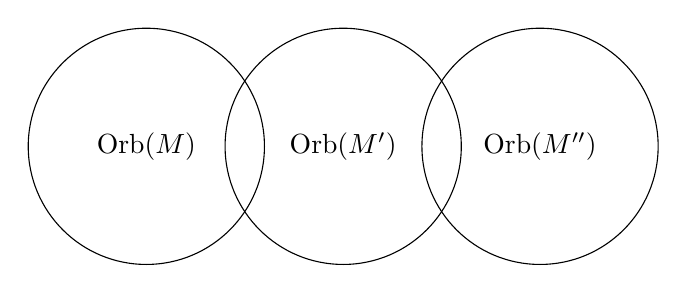
\begin{tikzpicture}[baseline=-0.25cm]
\draw (-2.5,0) circle (1.5) (-2.5,0)  node [text=black] {$\textup{Orb}(M)$};
\draw (0,0) circle (1.5) (0,0)  node [text=black] {$\textup{Orb}(M')$};
\draw (2.5,0) circle (1.5) (2.5,0) node [text=black] {$\textup{Orb}(M'')$};
\end{tikzpicture}.
\end{center}
\noindent\\ This picture becomes much more insightful in light of \hyperref[ActionPreorder]{Lemma \ref*{ActionPreorder}} and \hyperref[Transitive2]{Proposition \ref*{Transitive2}}.\\

%\noindent\textcolor{red}{Transitivity seems to be a stronger condition than being indecomposable. Note that being indecomposable means that, given any object $M \in \obset(\mathcal{M})$, we can

% In order to show that indecomposable implies transitive, we would need to be able to show that the orbit $\textup{Orb}(M)$ of each object $M \in \obset(\mathcal{M})$ cannot overlap with $\textup{Orb}(M')$ of any $M' \in \obset(\mathcal{M})\setminus\obset(\textup{Orb}(M))$, except at zero; that is, orbits are either disjoint or they coincide. Then we can use contradiction.}\\

\noindent\begin{definition}\textup{($\mathscr{C}$-Stable Ideal).} Let $\textup{M}$ be a birepresentation of $\mathscr{C}$. A %{\em left} (respectively {\em right}, {\em two-sided})
{\em $\mathscr{C}$-stable ideal} $\textup{I}$ of $\textup{M}$ is a collection $\textup{I} \coloneqq \{\textup{I}(\textobj{i}) : \textobj{i} \in \obset(\mathscr{C})\}$, where each $\textup{I}(\textobj{i})$ is a %left (respectively right, two-sided)
two-sided ideal of $\textup{M}(\textobj{i})$ such that $[\textup{M}(F)](\textup{I}(\textobj{i}))$ is a subclass of $\textup{I}(\textobj{j})$ for all $1$-morphisms $F \in \morset_\mathscr{C}^1(\textobj{i}, \textobj{j})$. %, for any morphism $\eta \in \textup{I}(\textobj{i})$ and any $1$-morphism $F \in \morset_\mathscr{C}^1(\textobj{i}, \textobj{j})$, we have that $[\textup{M}(F)](\eta) \in \textup{I}(\textobj{j})$.
%We say that $\textup{I}$ is {\em trivial} if, for all $\textobj{i} \in \obset(\mathscr{C})$, we have that either $\textup{I}(\textobj{i}) = \{0\}$ or $\textup{I}(\textobj{i}) = \morset(\textup{M}(\textobj{i}))$.\\
A $\mathscr{C}$-stable subideal $\textup{I}$ of a $\mathscr{C}$-stable ideal $\textup{J}$ is a $\mathscr{C}$-stable ideal for which $\textup{I}(\textobj{i})$ is a subideal of $\textup{J}(\textobj{i})$ for all $\textobj{i} \in \obset(\mathscr{C})$. We say that $\textup{I}$ is {\em proper} if there exists some $\textobj{i} \in \obset(\mathscr{C})$ for which $\textup{I}(\textobj{i})$ is proper, and {\em maximal} if it is proper and not a $\mathscr{C}$-stable subideal of any other proper $\mathscr{C}$-stable ideal.\\
\end{definition}

\noindent\begin{definition}\textup{(Simple Transitive Birepresentation).} %A multifinitary birepresentation of a multifinitary bicategory $\mathscr{C}$ is said to be {\em simple} (or {\em simple transitive}) if all of its $\mathscr{C}$-stable ideals are trivial.\\
A multifinitary birepresentation of a\linebreak multifinitary bicategory $\mathscr{C}$ is said to be {\em simple transitive} if it admits no proper, non-zero $\mathscr{C}$-stable ideals.\\
\end{definition}

\noindent Similarly to before, we say that a $\mathcal{C}$-module category $\mathcal{M}$ is simple transitive if its corresponding birepresentation is simple transitive. In other words, given non-zero $f, g \in \morset(\mathcal{M})$, we can obtain $g$ by composing $f$ with other morphisms in $\mathcal{M}$ and acting via $\mathcal{C}$ (by taking the left monoidal product).\\% with identity morphisms).\\

\noindent In light of the module category picture, we see that the ``right'' way to think about transitivity and simplicity is to observe that transitivity insists that your objects are cyclically generated (that is, $\textsf{add}(\{X \otimes M : X \in \obset(\mathcal{C})\}) = \obset(\mathcal{M})$ for all non-zero $X \in \obset(\mathcal{M})$), while simplicity insists that your morphisms are cyclically generated ($\{l \circ (\textup{id}_Y \otimes f) \circ r : Y \in \obset(\mathcal{C}), l, r \in \morset(\mathcal{M})\} = \morset(\mathcal{M})$ for all non-zero $f \in \morset(\mathcal{M})$)! This perspective, in addition to the following result, really elucidates our notion of simplicity for birepresentations.\newpage

%\noindent\textcolor{red}{Are there any well-known adjectives that transitive and simple are equivalent to? Is simple here the same as semisimple and indecomposable, the definition Pinhas uses? Probably not.}\\

\noindent\begin{proposition} Every simple transitive birepresentation is transitive.\\
\end{proposition}

\noindent\begin{proof} %Let $\textup{M}$ be a simple birepresentation of a multifinitary bicategory $\mathscr{C}$ and take $X \in \obset(\textup{M}(\textobj{i}))$ non-zero. Certainly $\textup{G}_\textup{M}(\{X\})$ induces a $\mathscr{C}$-stable ideal of $\textup{M}$, so it must be trivial by simplicity. In other words, for all $\textobj{j} \in \obset(\mathscr{C})$, we know that $\mathscr{C}_\textobj{j}(\{X\})$ must either be the trivial category $\{0\}$ or equivalent to $\textup{M}(\textobj{j})$.
%\textcolor{red}{Why is this non-zero when $X$ is non-zero? Supposedly we need the proof for lemma 3 of https://www2.math.uu.se/~vomaz677/PREPRINTS/VANESSA/transit.pdf, but the relevance of this makes no sense to me.} This completes the proof.
Let $\textup{M}$ be a simple transitive birepresentation of a multifinitary bicategory $\mathscr{C}$ and take $X \in \obset(\textup{M}(\textobj{i}))$ non-zero. Certainly $\textup{G}_\textup{M}(\{X\})$ induces a $\mathscr{C}$-stable ideal of $\textup{M}$ that is both non-empty and non-zero, as it contains $X$. Thus by the simplicity of $\textup{M}$, it follows that $\mathscr{C}_\textobj{j}(\{X\})$ must be equivalent to $\textup{M}(\textobj{j})$ for each $\textobj{j} \in \obset(\mathscr{C})$. Thus $\textup{M}$ is transitive. This completes the proof.
\end{proof}\\

\noindent It is not necessarily the case that transitive birepresentations are simple transitive! This will become clear when we look at certain subcategories of the Lusztig--Vogan module categories. However, transitive birepresentations can always be made simple transitive by leaving the objects alone and just throwing away some collection of morphisms. This result will end up being important in formulating the categorical version of the Jordan--H\"{o}lder theorem.\\ %(see https://arxiv.org/abs/0808.0764)
%Recall from \hyperref[YonedaBirepresentation]{Example \ref*{YonedaBirepresentation}} the Yoneda $2$-representation for $\mathscr{C}$ the monoidal delooping of $\textsf{Vect}$. The action of $\textup{M}$ is given by the tensor product; that is, $[\textup{M}(V)](U) \coloneqq V \otimes U$. Thus $\mathbb{P}_\bullet$ is naturally transitive, as the additive subcategory of vector space $V \otimes U$, for any non-zero vector spaces $V$ and $U$, is simply $\textsf{Vect}$. However, it is certainly not simple! To see why, suppose we let $A$ be any non-invertible two-dimensional matrix, and $\mathcal{I}(\mathbbm{k}^2, \mathbbm{k}^2)$ the algebra ideal generated by $A$. It's easy to see that this generates a proper, non-zero $\mathscr{C}$-stable ideal. \textcolor{red}{Pretty sure this is correct but it feels too easy, double check it!}\\

%\noindent\begin{proposition} A module category corresponds to a simple birepresentation if and only if \textcolor{red}{...}.\\
%\end{proposition}

%\noindent\begin{proof}
%\end{proof}\\

%\noindent Let $\mathscr{C}$ be a multifinitary bicategory and denote by $\mathcal{S}(\mathscr{C})$ the multisemigroup of isomorphism classes of $1$-morphisms in $\mathscr{C}$, as per \cite[section 3.3]{MM14}. We define on $\mathcal{S}(\mathscr{C})$ a left preorder $\geq_L$ by saying, for two $1$-morphisms $F, G \in \morset^1(\mathscr{C})$, that $F \geq_L G$ if and only if there is a $1$-morphism $H \in \morset^1(\mathscr{C})$ for which $F$ is isomorphic to a direct summand of $H \circ G$. We define an equivalence relation $\sim$ given by $F \sim G$ if and only if $F \geq_L G$ and $G \geq_L F$, and call equivalence classes under this relation {\em left cells}.\\

%\noindent Given some left cell $\mathcal{L}$ in $\mathscr{C}$, let $\textobj{i} \in \obset(\mathscr{C})$ be the object that is the domain for every $1$-morphism in $\mathcal{L}$. Moreover, for $\textobj{j} \in \obset(\mathscr{C})$, let $\textup{N}(\textobj{j})$ denote the additive closure in $\mathbb{P}_\textobj{i}(\textobj{j})$ of all $1$-morphisms $F \in \mathscr{C}(\textobj{i}, \textobj{j})$ for which $F \geq_L \mathcal{L}$. This induces a finitary subbirepresentation of $\mathbb{P}_\textobj{i}$ given by $\textup{N} : \textobj{j} \mapsto \textup{N}(\textobj{j})$.\\

%%%%%%%%%%%%%%%%%%%%%%%%%%%%%%%%%%%%%%%%%%%%%%%%%%
%%%%%%%%%%%%%%%%%%%%%%%%%%%%%%%%%%%%%%%%%%%%%%%%%%

%\noindent\begin{remark}\label{MatrixCalculus} Let $\mathcal{C}$ be an additive category. Then by \cite[\S VIII.2]{Mac13}, its morphisms form a matrix calculus; that is, for any $f \in \morset_\mathcal{C}(X, Y)$ with $X \cong \bigoplus_{i=1}^m{X_i}$ and $Y \cong \bigoplus_{j=1}^n{Y_j}$, we have that
%\begin{align*}
%\begin{split}
%f = \sum_{j=1}^n{\sum_{i=1}^m{(\iota_{Y_j} \circ f_{i,j} \circ \pi_{X_i})}}
%\end{split}
%\end{align*}
%\noindent for $f_{i,j} \coloneqq \pi_{Y_j} \circ f \circ \iota_{X_i}$, where $\pi_{X_i} : X \to X_i$ and $\pi_{Y_j} : Y \to Y_j$ are epimorphisms while $\iota_{X_i} : X_i \to X$ and\linebreak $\iota_{Y_j} : Y_j \to Y$ are monomorphisms for all $i \in \{1, \dots, m\}$ and $j \in \{1, \dots, n\}$.\\
%\end{remark}

%%%%%%%%%%%%%%%%%%%%%%%%%%%%%%%%%%%%%%%%%%%%%%%%%%
%%%%%%%%%%%%%%%%%%%%%%%%%%%%%%%%%%%%%%%%%%%%%%%%%%

%\noindent\begin{proposition} There is a unique maximal $\mathscr{C}$-stable ideal $\textup{I}$ in $\textup{N}$. Moreover, no $\textup{N}(\textobj{i})$ contains the identity morphism $\textup{id}_F$ for any $F \in \mathcal{L}$.\\
%\end{proposition}

\noindent\begin{lemma}\label{UniqueMaximalIdeal} Let $\textup{M}$ be a transitive birepresentation of a multifinitary bicategory $\mathscr{C}$. Then $\textup{M}$ admits a unique maximal $\mathscr{C}$-stable ideal $\textup{I}$, and moreover each $\textup{I}(\textobj{i})$ contains no identity morphisms apart from the one corresponding to the zero object.\\
\end{lemma}

\noindent\begin{proof} Let $\textup{I}$ be the sum %(as vector spaces)
of all $\mathscr{C}$-stable ideals of $\textup{M}$ that do not contain $\textup{id}_X$ for any non-zero $X \in \obset(\textup{M}(\textobj{i}))$ and any $\textobj{i} \in \obset(\mathscr{C})$. This is certainly itself a $\mathscr{C}$-stable ideal by construction. Moreover, because the sum of any two ideals $\mathcal{I}$ and $\mathcal{J}$ is an ideal containing both $\mathcal{I}$ and $\mathcal{J}$, it follows that %$U, V \subseteq U + V$ for vector spaces $U, V$, it follows that a sum of ideals is itself an ideal containing each ideal being summed, whence
$\textup{I}$ is maximal with respect to $\mathscr{C}$-stable ideals not containing identity morphisms. To see that it is genuinely maximal, suppose $\textup{J}$ is a $\mathscr{C}$-stable ideal containing $\textup{I}$. %We first note that by \hyperref[MatrixCalculus]{Remark \ref*{MatrixCalculus}}, each $\textup{J}(\textobj{i})$ will be uniquely determined by its morphisms between indecomposable objects, so we may restrict our focus to such morphisms.
Because $\textup{I}$ is maximal with respect to $\mathscr{C}$-stable ideals not containing identity morphisms, $\textup{J}$ must contain at least one identity morphism, say $\textup{id}_X$ for some non-zero $X \in \obset(\textup{M}(\textobj{i}))$. Given any non-zero $Y \in \obset(\textup{M}(\textobj{j}))$, the transitivity of $\textup{M}$ tells us that $Y$ is either isomorphic to a direct summand of $[\textup{M}(F)](X)$, for some $F \in \morset_\mathcal{C}^1(\textobj{i}, \textobj{j})$, or isomorphic to a direct sum $[\textup{M}(F_1)](X) \oplus \cdots \oplus [\textup{M}(F_n)](X)$, for some $F_1, \dots, F_n \in \morset_\mathcal{C}^1(\textobj{i}, \textobj{j})$. We claim that $\textup{id}_Y$ must lie in $\textup{J}(\textobj{j})$ in both cases.\\[-1.5\baselineskip]
\begin{center}
\rule{0.5\linewidth}{1pt}
\end{center}
\noindent\\[-\baselineskip]
\noindent Let $F \in \morset_\mathcal{C}^1(\textobj{i}, \textobj{j})$ with $[\textup{M}(F)](X) = X_1 \oplus \cdots \oplus X_n$ and suppose that $\varphi : Y \to X_k$ is an isomorphism for some $1 \leq k \leq n$. Then $[\textup{M}(F)](\textup{id}_X) = \textup{id}_{X_1 \oplus \cdots \oplus X_n} \in \textup{J}(\textobj{j})$ by $\mathscr{C}$-stability. But by pre-composing with $\iota_{X_k} \circ \varphi^{-1} : Y \to X_k \to X_1 \oplus \cdots \oplus X_n$ and post-composing with $\varphi \circ \pi_{X_k} : X_1 \oplus \cdots \oplus X_n \to X_k \to Y$, we obtain that $\textup{id}_Y = (\varphi \circ \pi_{X_k}) \circ \textup{id}_{X_1 \oplus \cdots \oplus X_n} \circ (\iota_{X_k} \circ \varphi^{-1}) \in \textup{J}(\textobj{j})$.\\[-1.5\baselineskip]
\begin{center}
\rule{0.5\linewidth}{1pt}
\end{center}
\noindent\\[-\baselineskip]
\noindent Suppose now that $\varphi : Y \to X_1 \oplus \cdots \oplus X_n$ is an isomorphism, where for each  $1 \leq k \leq n$ we have $X_k = [\textup{M}(F_k)](X)$ for some $F_k \in \morset_\mathcal{C}^1(\textobj{i}, \textobj{j})$. As before, $[\textup{M}(F_k)](\textup{id}_X) = \textup{id}_{X_k} \in \textup{J}(\textobj{j})$ for all $1 \leq k \leq n$ by $\mathscr{C}$-stability. Moreover, because $\textup{J}(\textobj{j})$ is an ideal, $\iota_{X_k} \circ \textup{id}_{X_k} \circ \pi_{X_k} = \iota_{X_k} \circ \pi_{X_k} \in \textup{J}(\textobj{j})$ for all $1 \leq k \leq n$. Thus by the definition of an additive category, $\textup{id}_{X_1 \oplus \cdots \oplus X_n} = \iota_{X_1} \circ \pi_{X_1} + \cdots + \iota_{X_n} \circ \pi_{X_n} \in \textup{J}(\textobj{j})$, whence it follows that $\textup{id}_Y = \varphi^{-1} \circ \textup{id}_{X_1 \oplus \cdots \oplus X_n} \circ \varphi \in \textup{J}(\textobj{j})$.\\[-1.5\baselineskip]
\begin{center}
\rule{0.5\linewidth}{1pt}
\end{center}
\noindent\\[-\baselineskip]
\noindent We have thus shown that $\textup{J}$ must contain {\em all} identity morphisms and therefore cannot be proper, meaning that $\textup{I}$ must in fact be maximal as claimed. The uniqueness of $\textup{I}$ follows by construction. This completes the proof.
%We claim that this $\mathscr{C}$-stable ideal is not only maximal, but the unique maximal ideal not containing non-zero identity morphisms. First, by \hyperref[MatrixCalculus]{Remark \ref*{MatrixCalculus}}, each $\textup{I}(\textobj{i})$ will be uniquely determined by its morphisms between indecomposable objects. Suppose therefore that we have some indecomposable $X \in \obset(\textup{M}(\textobj{i}))$; naturally, the corresponding unital algebra $\textup{End}_{\textup{M}(\textobj{i})}(X)$ of endomorphisms of $X$ is local by \hyperref[KrullSchmidt]{Theorem \ref*{KrullSchmidt}}. In other words, it admits a unique maximal ideal $J(X)$, known as the Jacobson radical. This ideal consists of all non-invertible elements of $\textup{End}_{\textup{M}(\textobj{i})}(X)$, and hence is the largest ideal that does not contain $\textup{id}_X$. But now we know that if we have any subideals of $J(X)$, then they are all subideals of their sum, which remains a subideal of $J(X)$; in other words, by extending this logic to every indecomposable object, we see that $\textup{I}$ is certainly maximal and does not contain any identity morphisms. That $\textup{I}$ is the unique $\mathscr{C}$-stable ideal with these properties follows directly from the uniqueness of each $J(X)$. This completes the proof.
\end{proof}\\

\noindent Let $\mathcal{C}$ be a preadditive category admitting a two-sided ideal $\mathcal{I}$. We define a congruence relation $\sim_\mathcal{I}$ on each $\mathcal{C}(X, Y)$ by $f \sim_\mathcal{I} g$ if and only if $f - g \in \mathcal{I}(X, Y)$. This motivates the following definition.\newpage

\noindent\begin{definition}\!\textup{(Quotient Category).}\label{QuotientCategory } Let $\mathcal{C}$ be a preadditive category admitting a two-sided ideal $\mathcal{I}$. We define the {\em quotient category} $\mathcal{C}/\mathcal{I}$ to be the subcategory whose classes of morphisms are given by $\mathcal{C}/\mathcal{I}(X, Y) \coloneqq \mathcal{C}(X, Y)/\!\sim_\mathcal{I}$, for all $X, Y \in \obset(\mathcal{C})$.\\%, and whose objects are those objects $X \in \obset(\mathcal{C})$ for which $\textup{id}_X \in \mathcal{C}/\mathcal{I}(X, X)$ (that is, for which $\mathcal{C}/\mathcal{I}(X, X) \neq \varnothing$).\\
\end{definition}

\noindent\begin{theoremdefinition}\!\textup{(Simple Quotient).}\label{SimpleQuotient} \!A transitive birepresentation $\textup{M}$ of a %\linebreak
multifinitary bicategory $\mathscr{C}$ is simple transitive if and only if the unique maximal $\mathscr{C}$-stable ideal $\textup{I}$ from \hyperref[UniqueMaximalIdeal]{Lemma \ref*{UniqueMaximalIdeal}} is the zero ideal. The simple transitive subbirepresentation $\underline{\textup{M}}$ of $\textup{M}$ that sends each object $\textobj{i} \in \obset(\mathscr{C})$ to the quotient subcategory $\textup{M}(\textobj{i})/\textup{I}(\textobj{i})$ is known as the {\em simple quotient} of $\textup{M}$.\\
\end{theoremdefinition}

\noindent\begin{proof} Naturally if $\textup{I}$ -- the sum of all $\mathscr{C}$-stable ideals without non-zero identity morphisms -- is the zero ideal, then $\textup{M}$ must contain no proper, non-zero $\mathscr{C}$-stable ideals. Conversely, if $\textup{M}$ is simple transitive, then because $\textup{I}$ is the sum of proper $\mathscr{C}$-stable ideals, they must all be zero. Finally, because $\textup{I}$ is maximal, every morphism $f \in \morset(\textup{M}(\textobj{i})/\textup{I}(\textobj{i}))$ must generate either $\{0\}$ or $\textup{M}(\textobj{i})/\textup{I}(\textobj{i})$ under composition with morphisms in $\mathscr{C}$, whence $\underline{\textup{M}}$ is simple transitive. This completes the proof.
\end{proof}\\

\noindent Let $\textup{M}$ be a multifinitary birepresentation of $\mathscr{C}$. We denote by $\textup{Ind}(\textup{M})$ the set of isomorphism classes of indecomposable objects in every $\textup{M}(\textobj{i})$, for $\textobj{i} \in \obset(\mathscr{C})$; that is,
\begin{align*}
\begin{split}
\textup{Ind}(\textup{M}) = \bigsqcup_{\textobj{i} \in \obset(\mathscr{C})} \{[X] \in \textup{M}(\textobj{i}) : \textup{$X$ is indecomposable}\}.
\end{split}
\end{align*}
\noindent Note that $\textup{Ind}(\textup{M})$ is clearly finite, as $\mathscr{C}$ has finitely many objects and each category $\textup{M}(\textobj{i}) \in \obset(\mathfrak{A}_\mathbbm{k}^f)$ has finitely many isomorphism classes of indecomposable objects.\\

\noindent For $X, Y \in \textup{Ind}(\textup{M})$, where for instance $X \in \textup{M}(\textobj{i}_X)$ and $Y \in \textup{M}(\textobj{i}_Y)$, we write $Y \geq X$ if there exists a $1$-morphism $F \in \morset_\mathscr{C}^1(\textobj{i}_X, \textobj{i}_Y)$ such that $Y$ is isomorphic to a direct summand of $[\textup{M}(F)](X)$.\\

\noindent\begin{lemma}\label{ActionPreorder} Let $\textup{M}$ be a multifinitary birepresentation. The binary relation $\geq$ defined above defines a preorder on $\textup{Ind}(\textup{M})$ known as the {\em action preorder}.\\
\end{lemma}

\noindent\begin{proof} Clearly $\geq$ is reflexive, as we can just take $F \coloneqq \textup{id}_\textobj{i}$. Moreover, suppose that $X$ is isomorphic to a direct summand of $[\textup{M}(F)](Y)$ and $Y$ is isomorphic to a direct summand of $[\textup{M}(G)](Z)$; that is,
\begin{align*}
\begin{split}
[\textup{M}(F)](Y) &\cong X \oplus X_1 \oplus X_2 \oplus \cdots,\\
[\textup{M}(G)](Z) &\cong Y \oplus Y_1 \oplus Y_2 \oplus \cdots.
\end{split}
\end{align*}
\noindent In order to show transitivity, we would like to show that $X$ is isomorphic to a direct summand of $[\textup{M}(FG)](Z)$. Well, because the morphisms of $\mathfrak{A}_\mathbbm{k}^f$ are additive, we simply observe that
\begin{align*}
\begin{split}
[\textup{M}(FG)](Z) &\cong [\textup{M}(F)](Y) \oplus [\textup{M}(F)](Y_1) \oplus [M(F)](Y_2) \oplus \cdots\\
&\cong X \oplus X_1 \oplus X_2 \oplus \cdots \oplus [\textup{M}(F)](Y_1) \oplus [\textup{M}(F)](Y_2) \oplus \cdots.
\end{split}
\end{align*}
\noindent This completes the proof.
\end{proof}\\

\noindent Suppose we define an equivalence relation $\sim$ given by $X \sim Y$ if and only if $X \geq Y$ and $Y \geq X$. Obviously $\geq$ extends to a partial order on $\textup{Ind}(\textup{M})/\!\sim$. In particular, we have the following result.\newpage

\noindent\begin{proposition}\label{Transitive2} Let $\textup{M}$ be a multifinitary birepresentation. Then $\textup{M}$ is transitive if and only if\linebreak $\textup{Ind}(\textup{M})/\!\sim$ has only one element.\\
\end{proposition}

\noindent\begin{proof} Suppose $\textup{Ind}(\textup{M})/\!\sim$ is a singleton and take any $X \in \obset(\textup{M}(\textobj{i}))$ non-zero as a representative. Then for any indecomposable $Y \in \obset(\textup{M}(\textobj{j}))$, there exists some $F \in \morset_\mathscr{C}^1(\textobj{i}, \textobj{j})$ for which $Y$ is isomorphic to a direct summand of $[M(F)](X)$, since $Y \geq X$. In other words, the additive subcategory $\mathscr{C}_\textobj{j}(\{X\})$ is equivalent to $\textup{M}(\textobj{j})$, as by definition it is closed under direct summands and direct sums. Thus $\textup{M}$ is transitive.\\[-1.5\baselineskip]
\begin{center}
\rule{0.5\linewidth}{1pt}
\end{center}
\noindent\\[-\baselineskip]
\noindent Conversely, suppose $\textup{M}$ is transitive, and consider any pair of indecomposables $X \in \obset(\textup{M}(\textobj{i}))$ and $Y \in \obset(\textup{M}(\textobj{j}))$. Because $\mathscr{C}_\textobj{j}(\{X\})$ is equivalent to $\textup{M}(\textobj{j})$, we know by the definition of $\mathscr{C}_\textobj{j}(\{X\})$ that $Y$ is isomorphic to a direct summand of $[M(F)](X)$ for some $F \in \morset_\mathscr{C}^1(\textobj{i}, \textobj{j})$; that is, $Y \geq X$. The same argument applied to $\mathscr{C}_\textobj{i}(\{Y\})$ shows us that $X \geq Y$, whence $\textup{Ind}(\textup{M})/\!\sim$ has only one element. This completes the proof.
\end{proof}\\

\noindent\begin{definition}\textup{(Directed Order Ideal).} A {\em directed order coideal} of a partially ordered set $(P, \geq)$ is a non-empty subset $I$ such that
\begin{enumerate}[label=$\bullet$, leftmargin=4\parindent]
\item for all $x \in I$ and $y \in P$, $y \geq x$ implies that $y \in I$ (upper set);
\item for all $x, y \in I$, there is some $z \in I$ such that $x \geq z$ and $y \geq z$ (downward directed set).\\
\end{enumerate}
%\noindent A {\em coideal} of a partially ordered set $(P, \leq)$ is a subset that is an upper set and a downward directed set.\\
\end{definition}

\noindent\begin{remark} This definition is slightly unusual. It is more typical to talk of {\em directed order ideals} of partially ordered sets $(P, \leq)$, which are non-empty subsets that are lower sets and upward directed sets. We have chosen to use coideals rather than ideals due to how we have defined our partial order; the standard notion of a directed order ideal goes ``downwards'', while we want to go ``upwards''. To more explicitly illustrate why we have made this choice, suppose we have some $\mathcal{C}$-module category of $R$-modules with indecomposables $R, X \in \obset(\mathcal{C})$. Naturally we would expect $X \geq R$, and indeed with our setup this will be true, as we can always consider the functor $\textup{M}(X) = - \otimes_R X$.\\
%The reasoning behind this somewhat quirky setup will hopefully become clear once we look at some explicit examples of Jordan--H\"{o}lder filtrations.\\
%In the literature, this partial order is often written as $X \geq Y$ if there exists a $1$-morphism $F \in \morset_\mathscr{C}^1(\textobj{i}_Y, \textobj{i}_X)$ such that $X$ is isomorphic to a direct summand of $[\textup{M}(F)](Y)$; that is, the inequality symbol is the other way around. As a result, they consider {\em coideals} (non-empty subsets that are upper sets and downward directed sets) rather than ideals in what follows. This is because we want to go ``downwards'', in the sense that we collect all direct summands. \textcolor{red}{Why do they define the order ``backwards''? Is there some (cell?) interpretation for which that is more natural?}\\
\end{remark}

%\noindent\textcolor{red}{For what follows, we will be considering coideals rather than ideals; the reason is because we want to ``go upwards'' with respect to our equivalence relation. That is, if we have (the isomorphism class of) an indecomposable object $X$, we also want to have every object that, roughly speaking, is isomorphic to a direct summand of $X$ (perhaps after $X$ is acted on by $\mathscr{C}$). This ensures that we are closed under taking direct summands, even after an action by $\mathscr{C}$.}\newpage

\noindent Let $\textup{M}$ be a multifinitary birepresentation of $\mathscr{C}$ and $Q$ a directed order coideal of $\textup{Ind}(\textup{M})/\!\sim$. For $\textobj{i} \in \obset(\mathscr{C})$, define $\textup{M}_Q(\textobj{i})$ to be the additive subcategory of $\textup{M}(\textobj{i})$ generated by every indecomposable object $X \in \obset(\textup{M}(\textobj{i}))$ whose equivalence class lies in $Q$. Then $\textup{M}_Q : \textobj{i} \mapsto \textup{M}_Q(\textobj{i})$ induces a multifinitary subbirepresentation of $\textup{M}$, known as the subbirepresentation of $\textup{M}$ associated to $Q$.\\

\noindent Let $Q \subset R$ be a pair of directed order coideals in $\textup{Ind}(\textup{M})/\!\sim$ and let $\textup{I}_Q(\textobj{i})$ denote the ideal in $\textup{M}_R(\textobj{i})$ generated by the identity morphisms in $\textup{M}_Q(\textobj{i})$, for $\textobj{i} \in \obset(\mathscr{C})$. This collection of ideals is $\mathscr{C}$-stable, whence the multifinitary birepresentation $\textup{M}_R$ induces a multifinitary birepresentation $\textup{M}_{R/Q} : \textobj{i} \mapsto \textup{M}_R(\textobj{i})/\textup{I}_Q(\textobj{i})$. This is known as the quotient of $\textup{M}$ associated to $Q \subset R$. Note that if $\abs{R \setminus Q} = 1$, then $\abs{\textup{Ind}(\textup{M}_{R/Q})/\!\sim} = 1$, so $\textup{M}_{R/Q}$ will be transitive by \hyperref[Transitive2]{Proposition \ref*{Transitive2}}.\\

\noindent Choose $r \in \textup{Ind}(\textup{M})/\!\sim$ and let $X_r$ be the maximal directed order coideal in $\textup{Ind}(\textup{M})/\!\sim$ that does not contain $r$. In other words, $(\textup{Ind}(\textup{M})/\!\sim)\setminus X_r$ -- the complement of $X_r$ -- has maximal element $r$. %\textcolor{red}{Why do they also say $r$ is {\em minimal} in the complement of $X_r$ despite their order being backwards to mine?}
Thus we also obtain a directed order coideal $Y_r \coloneqq X_r \cup \{r\}$, as $r$ being maximal in the complement means $Y_r$ will be an upper set, whence the associated quotient $\textup{M}_{Y_r/X_r}$ is transitive by \hyperref[Transitive2]{Proposition \ref*{Transitive2}}. We henceforth let $\underline{\textup{M}}_r$ denote the simple quotient $\underline{\textup{M}}_{Y_r/X_r}$.\newpage

%\noindent Before stating the main theorem of this section, we recall the classical Jordan--H\"{o}lder theorem for modules over rings. Let $M$ be an $R$-module admitting the two composition series
%\begin{align*}
%\begin{split}
%\{0\} = M_0 \subset M_1 \subset \cdots \subset M_n = M,%
%\end{split}
%\end{align*}
%%\noindent and
%\begin{align*}
%\begin{split}
%\{0\} = M_0' \subset M_1' \subset \cdots \subset M_m' = M,
%\end{split}
%\end{align*}
%\noindent where by {\em composition series} we mean that these are filtrations of submodules where the {\em composition factors} $L_i \coloneqq M_i/M_{i-1}$ and $L_i' \coloneqq M_j'/M_{j-1}'$ are simple for all $i \in \{1, \dots, n\}$ and $j \in \{1, \dots, m\}$. The {\em Jordan--H\"{o}lder theorem} tells us that the {\em composition lengths} are equal -- that is, $n = m$ -- and moreover that there exists a permutation $\sigma \in S_n$ such that $L_i \cong L_{\sigma(i)}'$ for all $i \in \{1, \dots, n\}$.\\

\noindent Consider a filtration of directed order coideals
\begin{align*}
\begin{split}
\varnothing = Q_0 \subset Q_1 \subset \cdots \subset Q_n = \textup{Ind}(\textup{M})/\!\sim
\end{split}
\end{align*}
\noindent such that $\abs{Q_i \setminus Q_{i-1}} = 1$ for all $i \in \{1, \dots, n\}$. We call this a {\em complete filtration}. As shown previously, from such a filtration we have a corresponding {\em weak Jordan--H\"{o}lder series}
\begin{align*}
\begin{split}
\{0\} = \textup{M}_{Q_0} \subset \textup{M}_{Q_1} \subset \cdots \subset \textup{M}_{Q_n} = \textup{M}
\end{split}
\end{align*}
\noindent consisting of subbirepresentations whose {\em weak composition quotients} $\textup{L}_i \coloneqq \underline{\textup{M}}_{Q_i/Q_{i-1}}$ are simple transitive birepresentations for all $1 \leq i \leq n$. We are now ready to state \cite[Theorem 8]{MM16}.\\

\noindent\begin{theorem}\label{JordanHolder}\textup{(Weak Jordan--H\"{o}lder Theorem).} Let $\textup{M}$ be a multifinitary birepresentation of a\linebreak multifinitary bicategory $\mathscr{C}$ admitting the two complete filtrations
\begin{align*}
\begin{split}
\varnothing = Q_0 \subset Q_1 \subset \cdots \subset Q_n = \textup{Ind}(\textup{M})/\!\sim,%
\end{split}
\end{align*}
%\noindent and
\begin{align*}
\begin{split}
\varnothing = Q_0' \subset Q_1' \subset \cdots \subset Q_m' = \textup{Ind}(\textup{M})/\!\sim,
\end{split}
\end{align*}
\noindent with weak composition quotients $\{\textup{L}_i\}_{i=1}^n$ and $\{\textup{L}_j'\}_{j=1}^m$ respectively. Then $m = n$, and moreover there exists a permutation $\sigma \in S_n$ such that $\textup{L}_i$ and $\textup{L}_{\sigma(i)}'$ are equivalent for all $i \in \{1, \dots, n\}$.\\
\end{theorem}

\noindent\begin{proof} We clearly have $m = n = \abs{\textup{Ind}(\textup{M})/\!\sim}$ by the definition of a complete filtration. Suppose now that $r \in \textup{Ind}(\textup{M})/\!\sim$; then there exist unique $i, j \in \{1, 2, \dots, n\}$ for which $Q_i\setminus Q_{i-1} = Q_j'\setminus Q_{j-1}' = \{r\}$. If we can show that the birepresentations $\textup{L}_i$ and $\textup{L}_j'$ are both equivalent to $\underline{\textup{M}}_r$, then we are done. In particular, by symmetry it is enough to show that $\textup{L}_i$ is equivalent to $\underline{\textup{M}}_r$.\\[-1.5\baselineskip]
\begin{center}
\rule{0.5\linewidth}{1pt}
\end{center}
\noindent\\[-\baselineskip]
%\noindent Let $\textup{I}_{X_r}$ be the $\mathscr{C}$-stable ideal in $\textup{M}_{Y_r}$ for which $\textup{M}_{Y_r/X_r} = \textup{M}_{Y_r}/\textup{I}_{X_r}$ and $\textup{I}_{Q_{i-1}}$ the $\mathscr{C}$-stable ideal in $\textup{M}_{Q_i}$ for which $\textup{M}_{Q_i/Q_{i-1}} = \textup{M}_{Q_i}/\textup{I}_{Q_{i-1}}$. Since $\{r\} = Q_i\setminus Q_{i-1}$, we know by construction that $Q_{i-1} \subseteq X_r$, as $X_r$ is by definition the maximal directed order coideal not containing $r$; similarly, $Q_i \subseteq Y_r$. This second inclusion induces a faithful pseudonatural transformation from $\textup{M}_{Q_i}$ to $\textup{M}_{Y_r}$ that takes each $\textobj{i} \in \obset(\mathscr{C})$ to the full subcategory inclusion functor $\Phi_\textobj{i} : \textup{M}_{Q_i}(\textobj{i}) \to \textup{M}_{Y_r}(\textobj{i})$ and each $Z \in \obset(\mathscr{C}(\textobj{i}, \textobj{j}))$ to the canonical natural isomorphism $\Phi_Z : \Phi_\textobj{j} \circ \textup{M}_{Q_i}(Z) \Rightarrow \textup{M}_{Y_r}(Z) \circ \Phi_\textobj{j}$.
\noindent \textcolor{red}{Let $\textup{I}_{X_r}$ be the $\mathscr{C}$-stable ideal in $\textup{M}_{Y_r}$ for which $\textup{M}_{Y_r/X_r} = \textup{M}_{Y_r}/\textup{I}_{X_r}$ and $\textup{I}_{Q_{i-1}}$ the $\mathscr{C}$-stable ideal in $\textup{M}_{Q_i}$ for which $\textup{M}_{Q_i/Q_{i-1}} = \textup{M}_{Q_i}/\textup{I}_{Q_{i-1}}$. Since $\{r\} = Q_i\setminus Q_{i-1}$, we know by construction that $Q_{i-1} \subseteq X_r$, as $X_r$ is by definition the maximal directed order coideal not containing $r$; similarly, $Q_i \subseteq Y_r$. This second inclusion induces a pseudonatural transformation from $\textup{M}_{Q_i}$ to $\textup{M}_{Y_r}$ (a collection of natural isomorphisms from functors between Hom-categories to functors between Hom-subcategories), whence the first inclusion induces a pseudonatural transformation $\sigma : \textup{M}_{Q_i} \Rightarrow \textup{M}_{Y_r/X_r}$ by taking the quotient. Now, $\textup{M}_{Q_i}/\textup{I}_{Q_{i-1}}$ contains only the objects generated by indecomposables in the equivalence class $r$. But for any such pair of indecomposable objects $X, Y \in \obset(\textup{M}(\textobj{j}))$ lying in the equivalence class $r$, we have that $\textup{I}_{X_r}(X, Y) \subseteq \textup{I}_{Q_{i-1}}(X, Y)$ by the aforementioned inequalities. Thus the pseudonatural transformation $\sigma$ factors through $\textup{M}_{Q_i/Q_{i-1}}$, in the sense that there exist lax natural transformations $\sigma_1 : \textup{M}_{Q_i} \Rightarrow \textup{M}_{Q_i/Q_{i-1}}$ and $\sigma_2 : \textup{M}_{Q_i/Q_{i-1}} \Rightarrow \textup{M}_{Y_r/X_r}$ such that $\sigma = \sigma_2 \circ \sigma_1$. In particular, this gives us a lax natural transformation $\sigma_2 : \textup{M}_{Q_i/Q_{i-1}} \Rightarrow \textup{M}_{Y_r/X_r}$ that is obviously surjective on morphisms by fullness; therefore, because $\textup{M}_{Q_i/Q_{i-1}}$ and $\textup{M}_{Y_r/X_r}$ are both transitive, taking their simple quotients via \hyperref[SimpleQuotient]{Theorem \ref*{SimpleQuotient}} induces an equivalence between $\textup{L}_i$ and $\underline{\textup{M}}_r$ as desired, whence the result follows. This completes the proof.}
\end{proof}\\

\noindent\textcolor{red}{I'm not happy with this proof, it's handwavey and I think I've got it wrong. Also, in what sense is this weak Jordan--H\"{o}lder theorem ``weak''? The decategorifications of these simple quotients are ``transitive $\mathbb{N}$-modules'' and usually not simple.}\\
\newpage

\ruledsection{Categories of Soergel Bimodules}{3}
\noindent\\ Throughout this chapter and the next, we will explore one of the main examples that has motivated the theory from the previous chapter: namely, categories of Soergel bimodules. %The upshot is as follows.
Given a Coxeter system $(W, S)$, we may define a corresponding Iwahori--Hecke algebra. These algebras appear all over mathematics, playing important roles in areas such as the representation theory of Lie groups and quantum groups, knot theory and statistical mechanics, among others. From this same Coxeter system, we may also construct a category of so-called Soergel bimodules, which is an algebraic categorification of the corresponding Iwahori--Hecke algebra. These categories were fundamental to the recent, purely algebraic proofs of the Kazhdan--Lusztig Conjecture (\cite[Conjecture 1.5]{KL79}) and Kazhdan--Lusztig Positivity Conjecture (\cite[p.\ 166]{KL79}) by Elias and Williamson (\cite[Theorem 1.1 and Corollary 1.2, respectively]{EW14}), and have since become an indispensable tool in Lie theory.\\
%First, however, we should provide some historical context. Our story starts in 1979, when Kazhdan and Lusztig introduced a family of polynomials arising from the Coxeter system corresponding to an Iwahori--Hecke algebra, now known as {\em Kazhdan--Lusztig polynomials}. They proposed that the algebraic characters of Verma modules -- certain representations of semisimple Lie algebras -- were related to the values of their associated Kazhdan--Lusztig polynomials at $1$ (\cite[Conjecture 1.5]{KL79}), hoping to address a\linebreak longstanding problem in representation theory. This conjecture came to be known as the\linebreak {\em Kazhdan--Lusztig conjecture}.\\

\noindent Before introducing categories of Soergel bimodules, we will briefly give definitions of Coxeter systems and Iwahori--Hecke algebras. We will not give much insight into these objects; for a more detailed survey, please see the wonderful book of Elias, Makisumi, Thiel and Williamson (\cite{EMTW20}).\\

\noindent\begin{definition}\textup{(Coxeter System).} Let $S$ be a finite set and $(m_{st})_{s,t \in S}$ a matrix satisfying
\begin{enumerate}[label=$\bullet$, leftmargin=4\parindent]
\item $m_{ss} = 1$, for each $s \in S$;
\item $m_{st} = m_{ts} \in \{2, 3, \dots\} \sqcup \{\infty\}$, for $s \neq t \in S$.
\end{enumerate}
%\begin{align*}
%\begin{split}
%m_{st} \in \begin{cases}\{1\},&s = t;\\\{2, 3, \dots\} \sqcup \{\infty\},&s \neq t.\end{cases}
%\end{split}
%\end{align*}
\noindent Consider now the subgroup $W$ of $F_S$, the free group over $S$, with presentation
\begin{align*}
\begin{split}
W &= \langle s \in S : \text{$(st)^{m_{st}} = 1$ for all $s, t \in S$ with $m_{st} < \infty$}\rangle.%\\
% &= \langle s \in S : \text{$s^2 = 1$, $(st)^{m_{st}} = (ts)^{m_{st}}$ for all $s, t \in S$ with $m_{st} < \infty$}\rangle.
\end{split}
\end{align*}
\noindent The pair $(W, S)$ is known as a {\em Coxeter system}, while $W$ %and any group $W$ admitting a Coxeter system
is known as a {\em Coxeter group}.\\
\end{definition}

\noindent We call the generating set $S$ the set of {\em simple reflections} and $(m_{st})_{s,t \in S}$ a {\em Coxeter matrix}. Because $s^2 = 1$ for all $s \in S$, the relation $(st)^{m_{st}} = 1$ is equivalent to the braid relation $sts\cdots = tst\cdots$ for all $s, t \in S$ with $m_{st} < \infty$, where both sides are the product of $m_{st}$ simple reflections.\\

\noindent\begin{definition}\textup{(Expression).} Let $(W, S)$ be a Coxeter system with $w \in W$. An {\em expression for $w$ of length $k$} is any sequence $\underline{w} := (s_1, \dots, s_k)$, for some not necessarily unique choice of $s_1, \dots, s_k \in S$, such that $w = s_1 s_2 \cdots s_k$. The {\em length} of $w$, denoted $\ell(w)$, is the length of its shortest expression, and any expression for $w$ of length $\ell(w)$ is said to be {\em reduced}. Moreover, $\ell(w) = 0$ if and only if $w = 1$.\\
\end{definition}

\noindent\begin{definition}\textup{(Bruhat Order).} Let $(W, S)$ be a Coxeter system and $\Phi \coloneqq \{wsw^{-1} : s \in S, w \in W\}$ the set of conjugates of simple reflections in $W$. For $x, y \in W$, we write $x \leq y$ if and only if there exists a chain $x = x_0, x_1, \dots, x_k = y$ such that $\ell(x_i) < \ell(x_{i+1})$ and $x_i^{-1}x_{i+1} \in \Phi$ for all $0 \leq i < k$. This defines a partial order on $W$, known as the {\em Bruhat order}.\\
\end{definition}

\noindent\begin{theorem}\label{Matsumoto}\textup{(Matsumoto's Theorem).} For any two reduced expressions of an element of a Coxeter group, the first can always be transformed into the second by repeatedly applying the braid relation.\\
\end{theorem}

\noindent This result was first shown in \cite{Mat64}. A sketch is given in \cite[Theorem 2.20]{EMTW20}, and the full proof can be found in \cite[Theorem 1.2.2]{GP00}.\newpage

\noindent\begin{definition}\textup{(Iwahori--Hecke Algebra).} Let $(W, S)$ be a Coxeter system and $v$ a formal variable. The {\em (one-parameter) Iwahori--Hecke algebra} corresponding to $(W, S)$ is the unital, associative\linebreak $\mathbb{Z}[v, v^{-1}]$-algebra $\mathscr{H}(W, S)$ with generators $\{\delta_s : s \in S\}$ and relations
\begin{enumerate}[label=$\bullet$, leftmargin=4\parindent]
\item (braid relation) $\delta_s\delta_t\delta_s\cdots = \delta_t\delta_s\delta_t\cdots$ for all $s, t \in S$ with $m_{st} < \infty$, where both sides are the product of $m_{st}$ generators;
\item (quadratic relation) $(\delta_s - v^{-1})(\delta_s + v) = 0$, for all $s \in S$.\\
\end{enumerate}
\end{definition}

\noindent Note that we can expand and rearrange the quadratic relation as $1 = \delta_s^2 + (v - v^{-1})\delta_s$, whence multiplying through by $\delta_s^{-1}$ gives us $\delta_s^{-1} = \delta_s + (v - v^{-1})$.\\

\noindent\begin{remark} If we identify our parameter $v$ with $1$, the Iwahori--Hecke algebra reduces to the group algebra $\mathbb{Z}W$. In other words, it is a deformation of the group algebra of its associated Coxeter group.\\
\end{remark}

\noindent\begin{remark} We have defined above the {\em one-parameter} Iwahori--Hecke algebra, as opposed to the more general {\em multiparameter} Iwahori--Hecke algebra, where instead of taking $\mathscr{H}(W, S)$ to be over the ring of one-parameter Laurent polynomials $\mathbb{Z}[v, v^{-1}]$ we consider a family of units $\{v_s : s \in S\}$ and take $\mathscr{H}(W, S)$ to be over the ring $\mathbb{Z}[v_s^{\pm 1} : s \in S]$.\\
\end{remark}

\noindent Let $(W, S)$ be a Coxeter system, and take $(s_1, \dots, s_\ell)$ and $(t_1, \dots, t_\ell)$ to be two reduced expressions for $w \in W$. Then $\delta_{s_1}\delta_{s_2}\cdots \delta_{s_\ell} = \delta_{t_1}\delta_{t_2} \cdots \delta_{t_\ell} \eqqcolon \delta_w$ by \hyperref[Matsumoto]{Matsumoto's Theorem} and the braid relation. In particular, by \cite[Theorem 3.5]{EMTW20}, the set $\{\delta_w : w \in W\}$ forms a $\mathbb{Z}[v, v^{-1}]$-basis for $\mathscr{H}(W, S)$ with $\delta_\textup{id} = 1$, known as the {\em standard basis}. Another important basis is the Kazhdan--Lusztig basis.\\

\noindent\begin{definition}\textup{(Kazhdan--Lusztig Involution).} Let $\mathscr{H}(W, S)$ be an Iwahori--Hecke algebra. The {\em Kazhdan--Lusztig involution} is the $\mathbb{Z}$-linear automorphism $h \mapsto \overline{h}$ on $\mathscr{H}(W, S)$, defined by
\begin{align*}
\begin{split}
\overline{\delta_s} \coloneqq \delta_s^{-1} = \delta_s + (v - v^{-1})
\end{split}
\end{align*}
\noindent on generators and by $\overline{v} = v^{-1}$ on Laurent polynomials. The {\em Kazhdan--Lusztig anti-involution} is the $\mathbb{Z}$-linear anti-automorphism $h \mapsto \omega(h)$ defined similarly on generators and Laurent polynomials.\\
\end{definition}

\noindent \noindent Given $w \in W$ admitting a reduced expression $(s_1, \dots, s_\ell)$, we find that
\begin{align*}
\begin{split}
\overline{\delta_w} &= \overline{\delta_{s_1}}\cdots\overline{\delta_{s_\ell}} = \delta_{s_1}^{-1}\cdots \delta_{s_\ell}^{-1} = (\delta_{w^{-1}})^{-1},\\
\omega(\delta_w) &= \overline{\delta_{s_\ell}}\cdots\overline{\delta_{s_1}} = \delta_{s_\ell}^{-1}\cdots \delta_{s_1}^{-1} = \delta_w^{-1}.\\
\end{split}
\end{align*}
\noindent With this, we are ready to define the Kazhdan--Lusztig basis.\\

\noindent\begin{theoremdefinition}\textup{(Kazhdan--Lusztig Basis).} Let $\mathscr{H}(W, S)$ be an Iwahori--Hecke algebra. Then it admits a unique $\mathbb{Z}[v, v^{-1}]$-basis $\{b_w : w \in W\}$ such that each $b_w$ satisfies
\begin{enumerate}[label=$\bullet$, leftmargin=4\parindent]
\item (self-duality) $\overline{b_w} = b_w$,
\item (degree bound) $b_w = \sum_{y \in W}{h_{y,w}(v) \delta_y}$,
\end{enumerate}
\noindent for some $h_{y,w}(v) \in v\mathbb{Z}_{\geq 0}[v]$ with $h_{w,w}(v) \coloneqq 1$ and $h_{y,w}(v) \coloneqq 0$ whenever $y \nleq w$ under the Bruhat order. This basis is known as the {\em Kazhdan--Lusztig basis}, and the polynomials $h_{y,w}$ are called {\em Kazhdan--Lusztig polynomials}.\\
\end{theoremdefinition}

\noindent A proof for existence can be found in \cite[Theorem 3.25]{EMTW20}, while a proof for uniqueness can be found in \cite[Lemma 3.10]{EMTW20}. A helpful example for $W = S_3$ is given in \cite[\S 3.3.1]{EMTW20}. Note that all coefficients of Kazhdan--Lusztig polynomials are non-negative; this is the aforementioned {\em Kazhdan--Lusztig Positivity Conjecture}, which was first proven for general Coxeter systems by Elias and Williamson in \cite[Corollary 1.2]{EW14}. Observe also that {\em any} set $\{b_w : w \in W\}$ satisfying the degree bound condition will be a basis; in particular, the Kazhdan--Lusztig polynomials induce a triangular change of basis matrix with $1$'s along the diagonal that maps the standard basis to $\{b_w : w \in W\}$, giving an isomorphism between the two sets.\\

\noindent\begin{definition}\textup{(Standard Form).} Let $\mathscr{H}(W, S)$ be an Iwahori--Hecke algebra. The {\em standard trace} $\tau : \mathscr{H}(W, S) \to \mathbb{Z}[v, v^{-1}]$ is the map that extracts the coefficient of $\delta_\textup{id}$; that is, it is the $\mathbb{Z}[v, v^{-1}]$-linear map for which $\tau(\delta_\textup{id}) = 1$ and $\tau(\delta_w) = 0$ for all $w \neq \textup{id}$. We then define the {\em standard form} on $\mathscr{H}(W, S)$ to be the sesquilinear form given by $(a, b) \coloneqq \tau(\omega(a)b)$, for all $a, b \in \mathscr{H}(W, S)$\\
\end{definition}

\noindent\begin{definition}\label{GeometricRepresentation}\textup{(Geometric Representation).} Let $(W, S)$ be a Coxeter system and $V$ the $\mathbbm{k}$-vector space with basis $\{\alpha_s : s \in S\}$, where $\textup{char}(\mathbbm{k}) = 0$. Define a symmetric, bilinear form on $V$ by% = \textup{span}_\mathbb{R}(\{\alpha_s : s \in S\})$ by
\begin{align*}
\begin{split}
(\alpha_s, \alpha_t) = \begin{cases}-\cos\!\left(\frac{\pi}{m_{st}}\right)\!,&m_{st} \neq \infty;\\-1,&m_{st} = \infty.\end{cases}
\end{split}
\end{align*}
\noindent From this, we define an action of $s \in S$ on the basis elements $\alpha_t \in V$ by the linear automorphism
\begin{align*}
\begin{split}
s(\alpha_t) \coloneqq \alpha_t - 2(\alpha_s, \alpha_t)\alpha_s,
\end{split}
\end{align*}
\noindent which reflects $\alpha_t$ across $\alpha_s$. The {\em geometric representation} of $(W, S)$ is the representation induced by linearly extending this reflection action to an action of $W$ on all of $V$.\\
\end{definition}

\noindent Let $(W, S)$ be a Coxeter system with geometric representation $V \coloneqq \textup{span}_\mathbbm{k}\{\alpha_s : s \in S\}$, and let $R := \textup{Sym}(V) = \bigoplus_{i=0}^\infty \textup{Sym}^i(V)$ 
%\begin{align*}
%\begin{split}
%R := \textup{Sym}(V) = \bigoplus_{i=0}^\infty \textup{Sym}^i(V)
%\end{split}
%\end{align*}
be the symmetric algebra of V, where $\textup{Sym}^i(V)$ is the {\em $i$th symmetric power of $V$}. We define this to be the quotient of the $i$th tensor power $V^{\otimes i}$ by the action of the symmetric group $S_i$, viewed as a $\mathbbm{k}$-module. For technical reasons we will take $R$ to be {\em graded in degree $2$}; that is, we will take all odd graded pieces to be $\{0\}$ and label $\textup{Sym}^i(V)$ as its $2i$th graded piece rather than its $i$th graded piece. We will comment more on why we do this in \hyperref[2Grading]{Remark \ref*{2Grading}} at the end of this chapter.\\

\noindent For the time being, let's try to understand what $\textup{Sym}^i(V)$ actually looks like. Let $S = \{s_1, s_2, \dots\}$, and observe that $V^{\otimes i}$ admits the basis $\{\alpha_{s_{j_1}} \otimes \cdots \otimes \alpha_{s_{j_i}} : s_{j_1}, \dots, s_{j_i} \in S\}$. We define an action of the symmetric group $S_i$ on basis elements in $V^{\otimes i}$ by $\sigma \cdot (\alpha_{s_{j_1}} \otimes \cdots \otimes \alpha_{s_{j_i}}) = (\alpha_{s_{\sigma(j_1)}} \otimes \cdots \otimes \alpha_{s_{\sigma(j_i)}})$, for $\sigma \in S_i$. This extends linearly to an action of $S_i$ on all of $V^{\otimes i}$. Thus quotienting by the action of the symmetric group has the effect of making $\otimes$ commutative; this can be seen clearly by considering finite $S$ and small $i$, for instance. Therefore, by linearly extending the map that sends basis elements $(\alpha_{s_{j_1}} \otimes \cdots \otimes \alpha_{s_{j_i}})$ to degree $i$ monomials $\alpha_{s_{j_1}} \cdots \alpha_{s_{j_i}}$, we obtain a $\mathbbm{k}$-module isomorphism from $\textup{Sym}^i(V)$ to the additive subgroup of the polynomial ring $\mathbbm{k}[\alpha_s : s \in S]$ consisting only of homogeneous degree $i$ polynomials. The upshot is that we may identify $R$ with the $\mathbb{Z}$-graded polynomial ring $\mathbbm{k}[\alpha_s : s \in S]$, whose $2i$th graded piece is the additive subgroup of homogeneous polynomials of degree $i$ for all non-negative $i$, with all other graded pieces being $\{0\}$.\newpage% (remembering that we are graded in degree $2$).\newpage

\noindent\begin{remark}\label{WRAction} Note that the reflection action of $W$ on $V$ given in \hyperref[GeometricRepresentation]{Definition \ref*{GeometricRepresentation}} induces an action of $W$ on $R$. This is given on monomials by $w(\alpha_{s_{j_1}} \cdots \alpha_{s_{j_i}}) = w(\alpha_{s_{j_1}}) \cdots w(\alpha_{s_{j_i}})$ and extended linearly to an action on all of $R$. Given a Coxeter group $(W, S)$ and some $I \subseteq S$, we denote by $W_I$ the subgroup of $W$ generated by $I$, known as the {\em (standard) parabolic subgroup generated by $I$}. We say that $I$ is {\em finitary} if $W_I$ is a finite group, and write $R^I \coloneqq \{f \in R : \text{$w(f) = f$ for all $w \in W_I$}\}$ for the set of $W_I$-invariant polynomials in $R$. Given $s \in S$, we will typically write $R^s$ rather than $R^{\{s\}}$; naturally, since $\langle g\rangle = \{g^n : n \in \mathbb{Z}\}$ for any element $g$ of an arbitrary group $G$, we have that $W_{\{s\}} = \{1, s\}$. Thus $R^s = \{f \in R : s(f) = f\}$, justifying our simplified notation.\\
\end{remark}

\noindent Before defining Soergel bimodules, we will introduce Bott--Samelson bimodules. As it happens, the category of Soergel bimodules is the graded closure of the Karoubian envelope of the category of Bott--Samelson bimodules. The easiest non-trivial example of a Bott--Samelson bimodule (and hence of a Soergel bimodule) is, given a Coxeter system $(W, S)$ and any $s \in S$, the graded $(R, R)$-bimodule\\[-1.1\linespacing]
\begin{align*}
\begin{split}
B_s \coloneqq R \otimes_{R^s} R(1),
\end{split}
\end{align*}
\noindent\\[-1.1\linespacing] where $(1)$ denotes a grading shift by $1$. By this we mean that $R(1)$ is a copy of $R$ whose $i$th graded piece is the $(i+1)$th graded piece of $R$. More generally, letting $R^i$ denote the $i$th graded piece of $R$, we have that $R(k)^i \coloneqq R^{i+k}$. Note that grading shifts commute with tensor products, and hence
\begin{align*}
\begin{split}
B_s = R \otimes_{R^s} R(1) = (R \otimes_{R^s} R)(1) = R(1) \otimes_{R^s} R.\\[\linespacing]
\end{split}
\end{align*}

\noindent\begin{definition}\textup{(Bott--Samelson Bimodule).} Let $(W, S)$ be a Coxeter system and $\underline{w} \coloneqq (s_1, \dots, s_k)$ an expression. The {\em Bott--Samelson bimodule corresponding to $\underline{w}$} is the graded $(R, R)$-bimodule
\begin{align*}
\begin{split}
BS(\underline{w}) &\coloneqq B_{s_1} \otimes_R \cdots \otimes_R B_{s_k}\\
&\hphantom{\coloneqq}\nhphantom{=}= (R \otimes_{R^{s_1}} R(1)) \otimes_R \cdots \otimes_R (R \otimes_{R^{s_k}} R(1))\\
&\hphantom{\coloneqq}\nhphantom{$\cong$}\cong R \otimes_{R^{s_1}} R \otimes_{R^{s_2}} \cdots \otimes_{R^{s_k}} R(k).
\end{split}
\end{align*}
\noindent We take the convention that if $\varnothing$ is the empty expression, then $BS(\varnothing) \coloneqq R$. Denote by $\mathbb{BS}\textcat{Bim}(W, S)$ the {\em category of Bott--Samelson bimodules corresponding to $(W, S)$}, whose objects are direct sums of Bott--Samelson bimodules corresponding to expressions in $(W, S)$ and whose morphisms are graded $(R, R)$-bimodule homomorphisms; that is, $(R, R)$-bimodule homomorphisms $\varphi : X \to Y$ that respect gradings, in the sense that $\varphi(X^i) \subseteq Y^i$ for all $i \in \mathbb{Z}$.\\
\end{definition}

\noindent Before we get too ahead of ourselves, a natural question we may ask is where these $B_s$ bimodules come from. Well, for any $s \in S$, one can verify that $R^s$ is generated by $\alpha_s^2$ and elements of the form $\alpha_t - (\alpha_s, \alpha_t)\alpha_s$, for $t \in S \setminus \{s\}$. This gives us a decomposition of $R$ into $s$-invariants and $s$-antiinvariants; that is, $R \cong R^s \oplus R^s \alpha_s \cong R^s \oplus R^s(-2)$ {\em as an $(R^s, R^s)$-bimodule}\footnote[2]{\ We will show this more explicitly later on, in \hyperref[RSplitting]{Lemma \ref*{RSplitting}}.}. Thus we have
\begin{align*}
\begin{split}
B_s \otimes_R B_s &= (R \otimes_{R^s} R(1)) \otimes_R (R \otimes_{R^s} R(1))\\
&\cong R \otimes_{R^s} R \otimes_{R^s} R(2)\\
&\cong R \otimes_{R^s} (R^s \oplus R^s(-2)) \otimes_{R^s} R(2)\\
&\cong (R \otimes_{R^s} R(2)) \oplus (R \otimes_{R^s} R)\\
&= B_s(1) \oplus B_s(-1).\\
\end{split}
\end{align*}
\noindent If we now look at the Kazhdan--Lusztig basis element $b_s$, it follows from uniqueness that $b_s = \delta_s + v$, as this is certainly a self-dual element satisfying the degree bound conditions for $s$. Thus
\begin{align*}
\begin{split}
b_s^2 &= \delta_s^2 + 2v\delta_s + v^2\\
&= (1 + (v^{-1} - v)\delta_s) + 2v\delta_s + v^2\\
&= 1 + v^{-1}\delta_s + v\delta_s + v^2\\
&= v(\delta_s + v) + v^{-1}(\delta_s + v)\\
&= vb_s + v^{-1}b_s.
\end{split}
\end{align*}
\noindent Comparing the expressions for $B_s$ and $b_s$, we see some striking similarities! This Bott--Samelson bimodule arising from the generator $s$ happens to behave just like an element of the Kazhdan--Lusztig basis, with positive (negative) grading shifts corresponding to multiplication (division) by our formal variable $v$. But what about the basis elements corresponding $w \in W\setminus S$? For these, Bott--Samelsons alone are insufficient. We therefore introduce Soergel bimodules.\\

\noindent\begin{definition}\textup{(Soergel Bimodule).} Let $(W, S)$ be a Coxeter system. A {\em Soergel bimodule} is a direct summand of a finite direct sum of grading shifts of Bott--Samelson bimodules corresponding to expressions in $(W, S)$. Denote by $\mathbb{S}\textsf{Bim}(W, S)$ the {\em category of Soergel bimodules corresponding to $(W, S)$}, which we define as the ``graded closure'' of the Karoubian envelope of $\mathbb{BS}\textcat{Bim}(W, S)$; in other words, it is the closure of the category of Bott--Samelson bimodules corresponding to $(W, S)$ under isomorphisms, direct summands, finite direct sums and grading shifts.\\
\end{definition}

\noindent\begin{remark} When we constructed $R$, we allowed $\mathbbm{k}$ to be any field of characteristic zero. In principle, this choice is completely arbitrary for $\mathbb{S}\textsf{Bim}$; this is one of the powers of Soergel bimodules! The field we choose to work over can be decided based on the context. In \cite{EMTW20}, this field is taken to be $\mathbb{R}$, as every symmetric $\mathbb{R}$-bilinear form is determined by its signature, a fundamental fact for doing Hodge theory. Alternatively, we will often be in the setting where we have some complex, semisimple Lie algebra $\mathfrak{g}$, along with a choice of Cartan subalgebra $\mathfrak{h}$ that determines a Weyl group $W$ and Borel subalgebra $\mathfrak{b}$ that determines a set of simple reflections $S$. In this setting, we will take $R$ to be the ring of regular functions on $\mathfrak{h}^*$% = \textup{spec}(R)$
, whence $R = \textup{Sym}(\mathfrak{h}) = \mathbb{C}[\alpha_s^\vee : s \in S]$ for coroots $\alpha_s^\vee \in \mathfrak{h}$ and $\mathfrak{h}^* = \textup{spec}(R)$. In this case, it is a result of Serre's theorem for quasicoherent sheaves that we can view $\mathbb{S}\textsf{Bim}(W, S)$ as a subcategory of the category of $\mathbb{C}^\times$-equivariant coherent sheaves of $\mathscr{O}_X$-modules on $X$, where $\mathscr{O}_X$ is the sheaf of regular functions on the pullback ${X \coloneqq \mathfrak{h}^* \times_{\mathfrak{h}^*/W} \mathfrak{h}^* = \textup{spec}(R \otimes_{R^{s,t}} R)}$.\\
\end{remark}

\noindent\begin{theorem}\textup{(Soergel's Categorification Theorem I).}\label{SoergelCategorification} There is a unique $\mathbb{Z}[v, v^{-1}]$-algebra\linebreak homomorphism $c : \mathscr{H}(W, S) \to \textup{Gr}(\mathbb{S}\textcat{Bim}(W, S))$ sending $v^k b_s$ to the isomorphism class $[B_s(k)]$, for each $s \in S$. Moreover, the $\Delta$-character function $\textup{ch}_\Delta : \mathbb{S}\textcat{Bim}(W, S) \to \mathscr{H}(W, S)$ descends to a homomorphism $\textup{ch} : \textup{Gr}(\mathbb{S}\textcat{Bim}(W, S)) \to \mathscr{H}(W, S)$ that is inverse to $c$, making these isomorphisms.\\
\end{theorem}

\noindent\begin{theorem}\textup{(Soergel's Categorification Theorem II).}\label{SBimIndecomposables} Let $(W, S)$ be a Coxeter system and $\underline{w}$ a reduced expression for $w \in W$. Then $BS(\underline{w})$ contains, up to isomorphism, a unique indecomposable summand $B_w$, which does not appear in $BS(\underline{x})$ for any $x < w$ and depends only on $w$, not the reduced expression. Moreover, all other direct summands are grading shifts of $B_x$, for $x < w$.\newpage
\end{theorem}

\noindent A statement of and reference for these results can be found in \cite[Theorem 5.24]{EMTW20}, as well as an algorithm for finding the indecomposables $B_w$. The precise definition of the $\Delta$-character function is $\textup{ch}_\Delta : B \mapsto \sum_{y \in W} v^{\ell(y)} h_y(B) \delta_y$, where $h_y(B) \in v\mathbb{Z}_{\geq 0}[v, v^{-1}]$ is some kind of graded multiplicity (this is slightly technical, see \cite[Theorem 5.10]{EMTW20} for details). For any indecomposable Soergel bimodule $B_w$, the graded multiplicities satisfy $h_y(B_w(k)) = v^k h_{y, w}(v)$ by Soergel's Conjecture.\\

\noindent\begin{corollary}\label{SBimIndecomposablesCardinality} The isomorphism classes of indecomposables of $\mathbb{S}\textcat{Bim}(W, S)$ are in bijection with $W \times \mathbb{Z}$.\\
\end{corollary}

\noindent\begin{proof} This follows from \hyperref[SBimIndecomposables]{Theorem \ref*{SBimIndecomposables}}, together with the fact that grading shifts preserve\linebreak indecomposability. In particular, the indecomposable objects are, up to isomorphism, grading shifts of $B_w$, for $w \in W$. This completes the proof.
\end{proof}\\

%\noindent\begin{remark}\label{GradedMultifinitary} Note that this means that we have infinitely many isomorphism classes of\linebreak indecomposable objects, and hence $\mathbb{S}\textsf{Bim}(W, S)$ is {\em not} multifinitary! However, we {\em can} say that it is {\em graded multifinitary}, as it is Krull--Schmidt and has finitely many indecomposables up to isomorphisms and grading shifts.\\
%\end{remark}

\noindent For any pre-additive category $\mathcal{C}$ with a {\em shift functor} -- that is, an additive, invertible endofunctor ${(1) : \mathcal{C} \to \mathcal{C}}$ -- we have that $\morset_\mathcal{C}(X(j), Y(i)) = \morset_\mathcal{C}(X, Y(i-j))$, where $X(k) \coloneqq [(1)^k](X)$. We define the corresponding {\em graded Hom-space} by $\morset^\bullet_\mathcal{C}(X, Y) \coloneqq \bigoplus_{i\in\mathbb{Z}} \morset_\mathcal{C}^i(X, Y)$, where the graded pieces are given by $\morset_\mathcal{C}^i(X, Y) \coloneqq \morset_\mathcal{C}(X, Y(i))$. In other words, this process endows $\mathcal{C}$ with the structure of a {\em graded category} -- a category whose Hom-spaces are $\mathbb{Z}$-graded Abelian groups. Similarly, we can turn any graded category into a category with a shift functor, and in fact by \cite[Proposition 11.9]{EMTW20} we have a pair of mutually adjoint pseudofunctors
\begin{center}
\begin{tikzcd}
\left\{\!\!\begin{tabular}{c}categories with\\ a shift functor\end{tabular}\!\!\right\}\arrow[rr, bend right=-40, "(-)^\textup{gr}"] && \left\{\!\!\begin{tabular}{c}graded\\ categories\end{tabular}\!\!\right\}\arrow[ll, bend left=40, "(-)^\textup{sh}"]
\end{tikzcd}
\end{center}
\noindent In other words, we can always think of the Hom-spaces of $\mathbb{S}\textcat{Bim}$ as being graded!\\

\noindent Now, given a finite-dimensional $\mathbb{Z}$-graded $\mathbbm{k}$-vector space $V = \oplus V^i$, we define its {\em graded dimension} to be the Hilbert--Poincar\'{e} series $\textup{gdim}(V) \coloneqq \sum_{i \in \mathbb{Z}}{\textup{dim}(V^i)v^i}$. Then given a free, finitely-generated left (respectively, right) graded $R$-module $M$, we define its {\em graded rank} to be $\textup{grk}(M) \coloneqq \textup{gdim}(\mathbbm{k} \otimes_R M)$ (respectively, $\textup{grk}(M) \coloneqq \textup{gdim}(M \otimes_R \mathbbm{k})$). Note that the purpose of tensoring with the underlying field here is to promote $M$ to a finite-dimensional $\mathbbm{k}$-vector space; since $M$ is finitely-generated, it admits a finite generating set $\{m_1, \dots, m_n\}$, whence $\{1 \otimes m_1, \dots, 1 \otimes m_n\}$ is a $\mathbbm{k}$-basis for $\mathbbm{k} \otimes_R M$.\\

\noindent\begin{theorem}\textup{(Soergel Hom Formula).}\label{SoergelHom} For any two Soergel bimodules $B, B' \in \mathbb{S}\textcat{Bim}(W, S)$, %the graded vector space
$\morset^\bullet_{\mathbb{S}\textcat{Bim}}(B, B')$ %\coloneqq \bigoplus_{i\in\mathbb{Z}} \morset_{\mathbb{S}\textcat{Bim}}(B, B'(i))$
is free as a left graded $R$-module and as a right graded $R$-module, both with\linebreak $\textup{grk}(\morset^\bullet_{\mathbb{S}\textcat{Bim}}(B, B')) = (\textup{ch}_\Delta(B), \textup{ch}_\Delta(B'))$, where $(-, -)$ denotes the standard form on $\mathscr{H}(W, S)$. In particular, the dimension of $\morset_{\mathbb{S}\textcat{Bim}}(B, B'(i))$ is given by the coefficient of $v^i$ in $(\textup{ch}_\Delta(B), \textup{ch}_\Delta(B'))$.\newpage
\end{theorem}

\noindent\begin{example} Consider the graded Hom-space $\morset^\bullet_{\mathbb{S}\textcat{Bim}}(B_s, B_s \otimes_R B_s)$. Since $\textup{ch}_\Delta(B_s) = b_s = \delta_s + v$ and $\textup{ch}_\Delta(B_s \otimes_R B_s) = b_s^2 = v^2 + v\delta_s + v^{-1}\delta_s + 1$, the standard form gives us
\begin{align*}
\begin{split}
(\textup{ch}_\Delta(B_s), \textup{ch}_\Delta(B_s \otimes_R B_s)) &= \tau(\omega(b_s)b_s^2) = \tau(b_s^3) = \tau((v + v^{-1})b_s^2) = \tau((v + v^{-1})^2b_s)\\
&= \tau((v + v^{-1})^2(\delta_s + v)) = (v + v^{-1})^2v\\
&= v^3 + 2v + v^{-1}.
\end{split}
\end{align*}
\noindent In other words, this tells us that as $\mathbbm{k}$-vector spaces, $\morset_{\mathbb{S}\textcat{Bim}}(B_s, B_s \otimes_R B_s(3))$ has dimension $1$, $\morset_{\mathbb{S}\textcat{Bim}}(B_s, B_s \otimes_R B_s(1))$ has dimension $2$ and $\morset_{\mathbb{S}\textcat{Bim}}(B_s, B_s \otimes_R B_s(-1))$ has dimension $1$, with all other graded pieces having dimension $0$. This is an extremely powerful result!\\
\end{example}


\noindent%\begin{remark}\label{SBimFiniteInd} 
Any category of Soergel bimodules is naturally a strict monoidal category. Although they are not Abelian, by the \hyperref[SoergelHom]{Soergel Hom Formula} we can view their classes of morphisms as finite-dimensional $\mathbbm{k}$-vector spaces by tensoring with $\mathbbm{k}$, and in fact one can show using \hyperref[KrullSchmidt1]{Theorem \ref*{KrullSchmidt1}} that they are Krull--Schmidt. By \hyperref[SBimIndecomposablesCardinality]{Corollary \ref*{SBimIndecomposablesCardinality}} it will only be {\em graded multifinitary}, as we only have finitely many indecomposable objects under both isomorphisms and grading shifts. Fortunately, however, the the only time having finitely many isomorphism classes of indecomposable objects comes into play is with the \hyperref[JordanHolder]{weak Jordan--H\"{o}lder Theorem}, where we only need $\textup{Ind}(\textup{M})/\!\sim$ to be finite.\\% But given a category $\mathcal{C}$ with a shift functor and any finitely-generated $\mathcal{C}$-module category $\mathcal{M}$, we know that we must have $X(k) \cong X(k) \otimes \mathbbm{1}_\mathcal{C} = X \otimes \mathbbm{1}_\mathcal{C}(k)$ for all $X \in \obset(\mathcal{M})$ and $k \in \mathbb{Z}$, whence $X \sim X(k)$.\\
%In general, if and in the case of $\mathbb{S}\textcat{Bim}(W, S)$ we have that $\textup{Ind}(\textup{M})/\!\sim$ is finite for any module category $\textup{M}$, since $X(k) \coloneqq X \otimes R(k)$ for all $X \in \obset(\mathcal{M})$ and $i, j \in \mathbb{Z}$, and hence $X \sim X(k)$ for all $k \in \mathbb{Z}$.\\ % In principle, the results of finitary birepresentation theory apply as long as our categories are (pre?)additive with finitely many equivalence classes of indecomposable objects.\\
%\end{remark}

\noindent\begin{theorem}\label{SoergelConjecture}\textup{(Soergel's Conjecture).} The isomorphism $\textup{ch} : \textup{Gr}(\mathbb{S}\textcat{Bim}(W, S)) \to \mathscr{H}(W, S)$ from \hyperref[SoergelCategorification]{Theorem \ref*{SoergelCategorification}} sends $B_w(k)$ to the isomorphism class $v^k b_w$, for each $w \in W$.\\
\end{theorem}

\noindent This result, which was first proven by Elias and Williamson (\cite[Theorem 1.1]{EW14}), generalizes the Kazhdan--Lusztig Conjecture and finally gives us an algebraic categorification of the Iwahori--Hecke algebra. This also means that our categories of Soergel bimodules are actually deceptively easy to work with; up to isomorphism, we can manipulate the objects by viewing them not as bimodules but as elements in the corresponding Iwahori--Hecke algebra. That said, Soergel bimodules also give us a collection of morphisms to look at. In fact, from the categorical perspective, the morphisms are really the items of interest -- compared to the Iwahori--Hecke algebra, they provide us with genuinely new information! As it turns out, even these morphisms are nice to work with, thanks to \hyperref[SoergelHom]{Theorem \ref*{SoergelHom}} and the fact that they admit a graphical calculus.\\

\noindent At this point, there are just a few loose ends that I'd like to tie up, which will hopefully become useful later on. Earlier we claimed that there exists an $(R^s, R^s)$-bimodule isomorphism $R \cong R^s \oplus R^s(-2)$ (which we note is certainly {\em not} an isomorphism of $(R, R)$-bimodules, as $R^s$ is itself not an $R$-module). I would like to show this more explicitly.\\

\noindent\begin{lemma}\label{RSplitting} For any $s \in S$ and $f \in R$, we have that $f + s(f) \in R^s$ and $f - s(f) \in R^s\alpha_s$. In particular, we have an $(R^s, R^s)$-bimodule splitting $R \cong R^s \oplus R^s\alpha_s \cong R^s \oplus R^s(-2)$ for every $s \in S$.\\
\end{lemma}

\noindent\begin{proof} Let $s \in S$ and $f \coloneqq \alpha_t$ for any $t \in S$. Observe that $g \coloneqq \frac{1}{2}(f + s(f)) = \alpha_t - (\alpha_s, \alpha_t)\alpha_s \in R^s$, while $h\alpha_s \coloneqq \frac{1}{2}(f - s(f)) = (\alpha_s, \alpha_t)\alpha_s \in R^s \alpha_s$. All that remains is to show that this holds for products. Suppose $f_1 \coloneqq g_1 + h_1\alpha_s$ and $f_2 \coloneqq g_2 + h_2\alpha_s$; %, for $g_1, h_1, g_2, h_2 \in R^s$.
then ${f \coloneqq f_1f_2 = g_1g_2 + g_1h_2\alpha_s + g_2h_1\alpha_s + h_1h_2\alpha_s^2}$ admits a unique decomposition of the form $g + h\alpha_s$, for $g \coloneqq \frac{1}{2}(f + s(f)) = g_1g_2 + h_1h_2\alpha_s^2$ and\linebreak $h\alpha_s \coloneqq \frac{1}{2}(f - s(f)) = g_1h_2\alpha_s + g_2h_1\alpha_s$. This completes the proof.
\end{proof}
\newpage

\noindent\begin{definition}\textup{(Demazure Operator).} For each $s \in S$, we define the corresponding {\em Demazure operator} to be the graded bimodule homomorphism $\partial_s : R \to R^s(-2)$ given by
\begin{align*}
\begin{split}
\partial_s : f \mapsto \frac{f - s(f)}{\alpha_s},
\end{split}
\end{align*}
for all $f \in R$.\\
\end{definition}

\noindent Clearly this map is well-defined by \hyperref[RSplitting]{Lemma \ref*{RSplitting}}. Essentially, the Demazure operators encapsulate the aforementioned splitting of $R$ into an $s$-invariant part and an $s$-antiinvariant part (in the sense that $s(f) = -f$). In particular, it is easy to see that for any $f \in R$, we have that $\partial_s(f\alpha_s) = f + s(f)$ while $\alpha_s\partial_s(f) = f - s(f)$. Thus we can rephrase our splitting in terms of Demazure operators as
\begin{align*}
\begin{split}
f = \partial_s\left(f\frac{\alpha_s}{2}\right) + \frac{\alpha_s}{2}\partial_s(f).
\end{split}
\end{align*}
\noindent As it happens, the Demazure operators have many nice properties.\\

\noindent\begin{lemma}\textup{(\cite[Lemma 4.15]{EMTW20}).} Let $s \in S$. Then
\begin{enumerate}[label=\textup{(\roman*).}, leftmargin=4\parindent]
\item $\partial_s$ is an $(R^s, R^s)$-bimodule map;
\item $s \circ \partial_s = \partial_s$ and $\partial_s \circ s = -\partial_s$;
\item $\partial_s \circ \partial_s = 0$;
\item there exists a short exact sequence
\begin{align*}
\begin{split}
0 \to R^s \to R \overset{\partial_s}{\to} R^s(-2) \to 0;
\end{split}
\end{align*}
\item (twisted Leibniz rule) $\partial_s(fg) = \partial_s(f)g + s(f)\partial_s(g)$, for all $f, g \in R$;
\item\label{DemazureBraid} (braid relation) for distinct simple reflections $s, t \in S$ with $m_{st} < \infty$,
\begin{align*}
\begin{split}
\partial_s \circ \partial_t \circ \partial_s \circ \cdots = \partial_t \circ \partial_s \circ \partial_t \circ \cdots,
\end{split}
\end{align*}
where both sides are the composition of $m_{st}$ Demazure operators.\\
\end{enumerate}
\end{lemma}

\noindent\begin{definition} The Demazure operator corresponding to $w \in W$ is given by
\begin{align*}
\begin{split}
\partial_w \coloneqq \partial_{s_1} \circ \cdots \circ \partial_{s_k},
\end{split}
\end{align*}
for any reduced expression $\underline{w} := (s_1, \dots, s_k)$ for $w$.\\
\end{definition}

\noindent By \hyperref[DemazureBraid]{(vi)} above and \hyperref[Matsumoto]{Matsumoto's Theorem}, this Demazure operator will not depend on the choice of reduced expression.\\

\noindent In the next chapter, we will be often find it helpful to view the dummy object in the monoidal delooping of $\mathbb{S}\textcat{Bim}$ as a category of modules over the {\em covariant algebra}. Let's briefly make some definitions for the purpose of preparing for this.\\

\noindent\begin{definition}\textup{(Reflection Faithful Representation).} Let $(W, S)$ be a Coxeter system. A faithful representation $\rho : W \to \textup{GL}(V)$ is further said to be {\em reflection faithful} if, for each $x \in W$, the corresponding fixed-point set $\{v \in V : [\rho(x)](v) = v\}$ has codimension $1$ if and only if $x$ is a {\em reflection} in $W$ (that is, $x$ is conjugate to an element of $S$).\\
\end{definition}
\newpage

\noindent In other words, we are asking that elements of $W$ act as reflections on $V$ if and only if they are reflections in $W$. Previously, our ring $R$ was defined in terms of the geometric representation, which is in general faithful but may fail to be reflection faithful (such as when $W$ is an affine Weyl group, for instance). For what follows, we will work with $R \coloneqq \textup{Sym}(V)$ for an arbitrary reflection faithful representation $(\rho, V)$.\\

%\noindent\begin{definition}\textup{(Realization).} Let $(W, S)$ be a Coxeter system and $\mathbbm{k}$ a commutative integral domain. Let $\mathfrak{h}$ be a free $\mathbbm{k}$-module of finite rank, together with a set $\{\alpha_s^\vee\}_{s \in S} \subseteq \mathfrak{h}$ of {\em simple coroots} and a set $\{\alpha_s\}_{s \in S} \subseteq \mathfrak{h}^* \coloneqq \homset_\mathbbm{k}(\mathfrak{h}, \mathbbm{k})$ of {\em simple roots}. Moreover, suppose that
%\begin{enumerate}[label=$\bullet$, leftmargin=4\parindent]
%\item $\alpha_s(\alpha_s^\vee) = 2$, for all $s \in S$;
%\item the map $S \times \mathfrak{h} \to \mathfrak{h}$ given by $(s, v) \mapsto v - \alpha_s(v)\alpha_s^\vee$ extends to a $W$-action on $\mathfrak{h}$;
%\item some minor technical conditions (see \cite[\S 5.7]{EMTW20}).
%\end{enumerate}
%\noindent The triple $(\mathfrak{h}, \{\alpha_s\}_{s \in S}, \{\alpha_s^\vee\}_{s \in S})$ is known as a {\em realization} of $(W, S)$.\\
%\end{definition}

\noindent\begin{definition}\textup{(Coinvariant Algebra).} Let $W$ be finite and denote by $R_+^{s,t}$ the graded subspace of $R^{s,t}$ consisting of everything in strictly positive degrees; that is,
\begin{align*}
\begin{split}
R_+^{s,t} \coloneqq \bigoplus_{i=1}^\infty R^i.
\end{split}
\end{align*}
\noindent Letting $I_W$ be the homogeneous ideal in $R$ generated by the elements in $R_+^{s,t}$, we define the {\em coinvariant algebra of $W$} to be the graded algebra
\begin{align*}
\begin{split}
C \coloneqq R/I_W.\\[\linespacing]
\end{split}
\end{align*}
\end{definition}

\noindent While this definition may seem a bit obtuse, the point is that we want to quotient out by the ideal generated by all of the {\em non-constant} $W$-invariant elements.\\ %\textcolor{red}{The point of defining this algebra is as follows. Any $W$-invariant polynomial $f \in R^W$ may pass through any tensor product $\otimes_{R^s}$ in a Bott--Samelson bimodule, and hence it will act the same on the left and right of any Soergel bimodule. Thus any $f \in R_+^W$ will act as zero on any Soergel module.}
\newpage

\noindent\begin{remark}\label{2Grading} In the following chapters, we will typically have a sequence of subgroups $T \subset B \subset G$, where $G$ is a connected, complex, reductive algebraic group, $B$ is a Borel subgroup and $T$ is a maximal torus. These inclusions induce a Weyl group $W \coloneqq N_G(T)/T$, where
\begin{align*}
\begin{split}
N_G(T) \coloneqq \{g \in G : gtg^{-1} \in T,\ \textup{for all $t \in T$}\};
\end{split}
\end{align*}
\noindent a set $\Phi = \Phi(G, T)$ of roots of $G$ relative to $T$; a set $S$ of simple roots of $W$ corresponding to $B$, such that $(W, S)$ is a Coxeter system (it is a fact that the set of Borel subgroups of $G$ containing $T$ are in bijection with the set of bases for $\Phi$); %a character lattice $\mathfrak{h}(T) \coloneqq \homset(T, \mathbb{C}^\times)$; a cocharacter lattice $\mathfrak{h}_*(T) \coloneqq \homset(\mathbb{C}^\times, T)$;
and a complex flag manifold (or generalized flag variety) $G/B$. Suppose now that we choose, for each $w \in W$, a representative $g_w \in N_G(T)$ for which $w = g_wT$. Letting $C_w \coloneqq Bg_wB$, which is well-defined since $T$ is a subgroup of $B$, we have the following stratification of $G$ into a disjoint union of $(B, B)$-double cosets:
\begin{align*}
\begin{split}
G = \bigsqcup_{w \in W} C_w.
\end{split}
\end{align*}
\noindent This is known as a {\em Bruhat decomposition} of $G$, and the double cosets $C_w$ are known as {\em Bruhat cells}. Importantly, this descends to a stratification of the flag variety $G/B$ in terms of {\em Schubert cells} of the form $X_w \coloneqq C_w/B$:
\begin{align*}
\begin{split}
G/B = \bigsqcup_{w \in W} X_w.
\end{split}
\end{align*}
\noindent The cells $X_w$ are locally closed subvarieties of $G/B$. We refer to the Zariski closure $\overline{X_w}$ as the {\em Schubert variety of $w$}, and remark that $\overline{X_y} \subseteq \overline{X_w}$ if and only if $y \leq w$. As an aside, we have that\\[-\linespacing]
\begin{align*}
\begin{split}
v^{\ell(w) - \ell(y)} h_{y,w}(v^{-1}) = \sum_{i \geq 0} v^i \textup{dim}_\mathbb{C}(IH^{2i}_{X_y}(\overline{X_w}, \mathbb{C})),
\end{split}
\end{align*}
\noindent\\[-0.7\linespacing] where $h_{y,w}$ is a Kazhdan--Lusztig polynomial for the Kazhdan--Lusztig basis of $\mathscr{H}(W, S)$. The term $IH^{2i}_{X_y}(X_w)$ is the stalk of the $i$th hypercohomology of $\textup{IC}_w$ at a (equivalently, any) point of $X_y$, where $\textup{IC}_w$ denotes the intersection cohomology sheaves of $\overline{X_w}$ (\cite[Theorem 13.13]{EMTW20}). This result was first shown in the appendix to \cite{KL79} (see Remark A11). One thing we may observe here is that we only sum over even graded pieces of the local intersection cohomology; the reason for this is that the odd graded pieces are all zero. In fact, because we have a left action of $B$ on $G/B$, we can consider the $B$-equivariant cohomology $H_B^*(G/B)$, which we will find is a ring that is also graded in degree $2$. As it turns out, $H_B^*(G/B) \cong R \otimes_{R^{s,t}} R$, which is why we grade $R$ the way that we do!\newpage
\end{remark}

\noindent\textcolor{red}{Go through the $SL_2$ and $SL_3$ examples in detail to put everything together, it'd be good to see an example of the Kazhdan--Lusztig basis of a Iwahori--Hecke algebra and compare it to the indecomposables in the corresponding category of Soergel bimodules. I should also start typing up Lie theory notes.}\\
\newpage

\noindent 

\newpage

\ruledsection{Simple Module Categories over Soergel Bimodules}{4}
\noindent\\ Before we talk about the Lusztig--Vogan module categories, it might be helpful to understand the classification result of Mackaay, Mazorchuk, Miemietz, Tubbenhauer and Zhang (\cite{MMMTZ23}). A family of birepresentations that play a particularly important role are cell birepresentations. In the context of Soergel bimodules, these module categories categorify Kazhdan--Lusztig cell representations of the Iwahori--Hecke algebra as a consequence of the \hyperref[SoergelConjecture]{categorification theorem}.\\

\noindent Let $\mathscr{C}$ be a multifinitary bicategory with indecomposables $F \in \obset(\mathscr{C}(\textobj{i}, \textobj{j}))$ and $G \in \obset(\mathscr{C}(\textobj{k}, \textobj{l}))$. We write $G \geq_L F$ if there exists some $H \in \obset(\mathscr{C}(\textobj{j}, \textobj{l}))$ for which $G$ is isomorphic to a direct summand of $H \circ F$ in the Hom-category $\mathscr{C}(\textobj{k}, \textobj{l})$ (note that this forces $\textobj{k} = \textobj{i}$). This is known as the {\em left preorder} (c.f. the \hyperref[ActionPreorder]{action preorder}). The set of equivalence classes of an indecomposable object $F$ is called the {\em left cell of $F$} and denoted $\mathcal{L}_F$. Similarly, we have a {\em right preorder} defined by $G \geq_R F$ if there exists some $H \in \obset(\mathscr{C}(\textobj{k}, \textobj{i}))$ for which $G$ is isomorphic to a direct summand of $F \circ H$, with equivalence classes known as {\em right cells} and denoted $\mathcal{R}_F$. Finally, we also write $G \geq_{J} F$ if there exist $H_l \in \obset(\mathscr{C}(\textobj{j}, \textobj{l}))$ and $H_r \in \obset(\mathscr{C}(\textobj{k}, \textobj{i}))$ for which $G$ is isomorphic to a direct summand of $H_l \circ F \circ H_r$, with equivalence classes known as {\em two-sided cells} and denoted $\mathcal{J}_F$. Such a cell is said to be {\em idempotent} if there exist $G, H, K \in \mathcal{J}_F$ such that $K$ is isomorphic to a direct summand of $G \circ H$.\\

%\noindent Note that if $X $ is isomorphic to a direct summand of $Y$, then it is isomorphic a direct summand of $\textup{id}_\textobj{j} \circ Y$, whence $X \geq_L Y$.\\

\noindent Let $\mathcal{L}_F$ be the left cell of $F \in \obset(\mathscr{C}(\textobj{s}, \textobj{t}))$ and define a multifinitary subbirepresentation $\textup{N}$ of the Yoneda birepresentation $\mathbb{P}_\textobj{s}$ given by restricting each $\mathbb{P}_\textobj{s}(\textobj{i}) = \mathscr{C}(\textobj{s}, \textobj{i})$ to the additive subcategory
\begin{align*}
\begin{split}
\textup{N}(\textobj{i}) \coloneqq \textcat{Add}(\{G \in \obset(\mathscr{C}(\textobj{s}, \textobj{i})) : G \geq_L \mathcal{L}_F\}).
\end{split}
\end{align*}
\noindent We will refer to this as the \textit{pre-cell birepresentation of $\mathscr{C}$ associated to $\mathcal{L}_F$}.\\

\noindent\begin{proposition}\label{UniqueMaximalIdealCell} Let $\textup{N}$ be the pre-cell birepresentation of a multifinitary bicategory $\mathscr{C}$ associated to a left cell $\mathcal{L}$. Then $\textup{N}$ admits a unique maximal $\mathscr{C}$-stable ideal $\textup{I}$, and moreover each $\textup{I}(\textobj{i})$ contains no identity morphisms corresponding to objects in $\mathcal{L}$.\\
\end{proposition}

\noindent\begin{sketch} The proof follows similarly to \hyperref[UniqueMaximalIdeal]{Lemma \ref*{UniqueMaximalIdeal}}, with $\textup{I}$ given by the sum of all $\mathscr{C}$-stable ideals of $\textup{N}$ that do not contain $\textup{id}_F$ for any $F \in \mathcal{L}$. Note that transitivity is no longer needed, as containing one such $\textup{id}_F$ means that you must contain $\textup{id}_G$ for all $G \in \mathcal{L}$ by $\mathscr{C}$-stability and the definition of left cells. Maximality also tells us that we must in fact include all identity morphisms corresponding to objects $F$ for which $F >_L \mathcal{L}$.
\end{sketch}\\

\noindent\begin{definition}\textup{(Cell Birepresentation).} Let $\textup{N}$ be the pre-cell birepresentation of a multifinitary bicategory $\mathscr{C}$ associated to a left cell $\mathcal{L}$. The simple transitive subbirepresentation $\mathscr{C}_\mathcal{L}$ of $\textup{N}$ that sends each object $\textobj{i} \in \obset(\mathscr{C})$ to the quotient subcategory $\textup{N}(\textobj{i})/\textup{I}(\textobj{i})$ is known as the {\em cell birepresentation} of $\mathscr{C}$ associated to $\mathcal{L}$.\\
\end{definition}

\noindent Unlike when going from transitive to simple transitive, going from pre-cell to cell typically annihilates objects. In particular, we will annihilate every object $F$ for which $F >_L \mathcal{L}$.\newpage

\noindent Let $\textup{M}$ be a birepresentation of $\mathscr{C}$. For any $X \in \obset(\textup{M}(\textobj{i}))$, we define
\begin{align*}
\begin{split}
\textup{Ann}_\mathscr{C}(X) \coloneqq \{F \in \obset(\mathscr{C}(\textobj{i}, \textobj{j})) : \textobj{j} \in \obset(\mathscr{C}), [\textup{M}(F)](X) = 0\}
\end{split}
\end{align*}
\noindent to be the {\em annihilator of $X$}. %This is a coideal with respect to $\geq_L$; that is, given $F \in \textup{Ann}_\mathscr{C}(M)$ and $G \geq_L F$, it is easy to see that $G \in \textup{Ann}_\mathscr{C}(M)$.
We define the {\em annihilator of $\textup{M}$} to be
\begin{align*}
\begin{split}
\textup{Ann}_\mathscr{C}(\textup{M}) \coloneqq \bigcap_{X} \textup{Ann}_\mathscr{C}(X),
\end{split}
\end{align*}
\noindent the collection of $1$-morphisms that are annihilated by $\textup{M}$.\\ %This is naturally a coideal with respect to $\geq_{LR}$, as if $F$ is annihilated by $\textup{M}$ then so too will any $H_2 \circ F \circ H_1$ and any direct summand of it.\\

\noindent\begin{definition}\textup{(Biideal).} A {\em left} (respectively {\em right}) {\em biideal} $\mathscr{I}$ of a bicategory $\mathscr{C}$ is a collection\linebreak $\mathscr{I} \coloneqq \{\mathscr{I}(\textobj{i}, \textobj{j}) : \textobj{i}, \textobj{j} \in \obset(\mathscr{C})\}$, where each $\mathscr{I}(\textobj{i}, \textobj{j})$ is a left (respectively right) ideal of the Hom-category $\mathscr{C}(\textobj{i}, \textobj{j})$ that is, in addition, stable under horizontal post-composition (respectively pre-composition). We say that $\mathscr{I}$ is a {\em two-sided biideal} if it is both a left biideal and a right biideal.\\
\end{definition}

\noindent The annihilator $\textup{Ann}_\mathscr{C}(\textup{M})$ gives us a two-sided biideal by taking all the $2$-morphisms between its $1$-morphisms. This in turn gives us a multifinitary bicategory $\mathscr{C}_\textup{M} \coloneqq \mathscr{C}/\textup{Ann}_\mathscr{C}(\textup{M})$ by quotienting each Hom-category. It is easy to see that the two-sided cells of $\mathscr{C}_\textup{M}$ are also two-sided cells of $\mathscr{C}$, although some two-sided cells of $\mathscr{C}$ may disappear from $\mathscr{C}_\textup{M}$ if they are annihilated by $\textup{M}$.\\

%\noindent It is easy to see that the two-sided cells of $\mathscr{C}_\textup{M}$ are also two-sided cells of $\mathscr{C}$, although some two-sided cells of $\mathscr{C}$ may disappear from $\mathscr{C}_\textup{M}$ if they are annihilated by $\textup{M}$. The set of all such two-sided cells that are annihilated by $\textup{M}$ together form an upper set in the poset $(\textup{Ind}(\mathscr{C}), \geq_{LR})$. This is because, for any $F \in \textup{Ann}_\mathscr{C}(\textup{M})$ and $G \in \textup{Ind}(\mathscr{C})$, we clearly have that $G \geq_{LR} F$ implies $G \in \textup{Ann}_\mathscr{C}(\textup{M})$.\\

\noindent\begin{lemmadefinition}\textup{(Apex).}\label{Apex} Let $\mathscr{C}$ be a multifinitary bicategory and $\textup{M}$ a transitive\linebreak birepresentation of $\mathscr{C}$. Then $\mathscr{C}_\textup{M}$ admits a unique maximal two-sided cell known as the {\em apex of $\textup{M}$}. Moreover, this two-sided cell is idempotent.\\
\end{lemmadefinition}

\noindent\begin{proof} For this proof, we will assume that $\mathscr{C}$ has only one object, $\bullet$. The more general proof follows similarly. We shall first proceed by contradiction. Let $\mathcal{J}_F$ and $\mathcal{J}_G$ be two different two-sided cells of $\mathscr{C}_\textup{M}$ that are maximal with respect to $\geq_{J}$, in the sense that $H \geq_{J} \mathcal{J}_F$ implies $\mathcal{J}_F \geq_{J} H$, and similarly for $\mathcal{J}_G$. Let $A$ (respectively $B$) be a multiplicity-free direct sum of representatives of $2$-isomorphism classes of indecomposable $1$-morphisms in $\mathcal{J}_F$ (respectively $\mathcal{J}_G$). In other words, $A = A_1 \oplus \dots \oplus A_m$ and $B = B_1 \oplus \cdots \oplus B_n$ are direct sums of indecomposable $1$-morphisms with each $2$-isomorphism class appearing exactly once. Note that we must have that $A \circ B = 0 = B \circ A$, as otherwise maximality would imply that $A = B$ (since $A \circ B \geq_{J} \mathcal{J}_F, \mathcal{J}_G$, for instance, where two cells with a non-empty intersection must be equal by transitivity of the preorder).\\[-1.5\baselineskip]
\begin{center}
\rule{0.5\linewidth}{1pt}
\end{center}
\noindent\\[-\baselineskip]
\noindent Let $X \coloneqq X_1 \oplus \cdots \oplus X_k$ now be a multiplicity-free direct sum of representatives of isomorphism classes of indecomposables in $\textup{M}({\bullet})$, whence $\textsf{add}(\{X\}) = \obset(\textup{M}({\bullet}))$. Naturally $[\textup{M}(A)](X) \neq 0$ by assumption, since $\mathcal{J}_F$ is a two-sided cell of $\mathscr{C}_\textup{M}$. Consider now any indecomposable summand $X'$ of $[\textup{M}(A)](X)$. Then because $\textup{M}$ is transitive, \hyperref[Transitive2]{Proposition \ref*{Transitive2}} tells us that there exists, for all $1 \leq i \leq k$, some $H_i \in \textup{Ind}(\mathscr{C})$ for which $X_i$ is isomorphic to a direct summand of $[\textup{M}(H_i \circ A)](X)$. Moreover, it follows from maximality that $H_i \circ A$ is a direct sum of indecomposables from $\mathcal{J}_F$, since it is clear that $F' \geq_{J} \mathcal{J}_F$ for any indecomposable summand $F'$ of some $H_i \circ A_j$. In other words,
\begin{align*}
\begin{split}
\textsf{add}(\{[\textup{M}(A)](X)\}) = \textsf{add}(\{[\textup{M}(H_1 \circ A)](X), \dots, [\textup{M}(H_k \circ A)](X)\}) = \textsf{add}(\{X\}),
\end{split}
\end{align*}
\noindent and similarly $\textsf{add}(\{[\textup{M}(B)](X)\}) = \textsf{add}(\{X\})$. These imply that $\textsf{add}(\{[\textup{M}(A \circ B)](X)\}) = \textsf{add}(\{X\})$, contradicting $A \circ B = 0$, whence the maximal two-sided cell must be unique. Finally, we see that $\textsf{add}(\{[\textup{M}(F \circ F)](X)\}) = \textsf{add}(\{[\textup{M}(F)](X)\}) = \textsf{add}(\{X\})$, meaning $F \circ F \neq 0$ and hence that $\mathcal{J}_F$ is idempotent. This completes the proof.
\end{proof}
\newpage

\noindent Lifting it back up to $\mathscr{C}$, \hyperref[Apex]{Lemma \ref*{Apex}} tells us that $\mathscr{C}$ admits a unique two-sided cell that is maximal among cells not annihilated by $\textup{M}$. Given a multifinitary bicategory $\mathscr{C}$ and a two-sided cell $\mathcal{J}$, let $\mathscr{C}\textup{-stmod}_\mathcal{J}$ denote the category of simple transitive birepresentations of $\mathscr{C}$ with apex $\mathcal{J}$.\\ %In \cite{MMMTZ23}, the simple transitive $2$-representations of $\mathbb{S}\textcat{Bim}$ are classified by their apexes. To keep notation clean, let $\mathscr{S} \coloneqq \mathbb{S}\textcat{Bim}$, and denote by $\mathscr{S}\textup{-(g)stmod}_\mathcal{A}$ the category of (graded) simple transitive $2$-representations of $\mathbb{S}\textcat{Bim}$ with apex $\mathcal{A}$.\\

\noindent In the context of \cite{MMMTZ23}, we can essentially perform the classification of simple transitive $2$-representations by looking at the apexes. In fact, we can take this reduction one step further via a technique known as {\em $\mathcal{H}$-reduction}.\\

\noindent\begin{definition}\textup{(Fiab Category).}\label{Fiab} A (multi)finitary bicategory $\mathscr{C}$ is said to be {\em quasi (multi)fiab} if it has adjunctions. In other words, if we have an object-preserving $\mathbbm{k}$-linear biequivalence ${}^* : \mathscr{C} \to \mathscr{C}^\textup{co,op}$ such that, for every $f \in \obset(\mathscr{C}(\textobj{i}, \textobj{j}))$, there exist adjunction $2$-morphisms $\textup{ev}_f : f \circ_h f^* \to \mathbbm{1}_\textobj{j}$ and $\textup{coev}_f : \mathbbm{1}_\textobj{i} \to f^* \circ_h f$ for which the diagrams
\begin{center}
\begin{tikzcd}
& f\arrow[dl, "r_f^{-1}"'] &\\
f \circ_h \mathbbm{1}_\textobj{i}\arrow[d, "\textup{id}_f \circ_h \textup{coev}_f"'] & & \mathbbm{1}_\textobj{j} \circ_h f\arrow[ul, "l_f"']\\
f \circ_h (f^* \circ_h f)\arrow[rr, "a_{f,f^*,f}^{-1}"'] & & (f \circ_h f^*) \circ_h f\arrow[u, "\textup{ev}_f \circ_h \textup{id}_f"']
\end{tikzcd}and\begin{tikzcd}
& f^*\arrow[dl, "l_{f^*}^{-1}"'] &\\
\mathbbm{1}_\textobj{i} \circ_h f^*\arrow[d, "\textup{coev}_f \circ_h \textup{id}_{f^*}"'] & & f^* \circ_h \mathbbm{1}_\textobj{j}\arrow[ul, "r_{f^*}"']\\
(f^* \circ_h f) \circ_h f^*\arrow[rr, "a_{f^*,f,f^*}"'] & & f^* \circ_h (f \circ_h f^*)\arrow[u, "\textup{id}_{f^*} \circ_h \textup{ev}_f"']
\end{tikzcd}
\end{center}
\noindent commute. If $\textnormal{id}_\mathscr{C}$ and $({}^*)^2$ are internally equivalent in $[\mathscr{C}, \mathscr{C}]$, then $\mathscr{C}$ is said to be {\em (multi)fiab}. The strict version of a (quasi) (multi)fiab bicategory is known as a {\em (quasi) (multi)fiat $2$-category}.\\
\end{definition}

\noindent\begin{definition}\textup{($\mathcal{J}$-Simplicity).} Let $\mathscr{C}$ be a multifinitary bicategory with $\mathcal{J}$ a two-sided cell. We say that $\mathscr{C}$ is {\em $\mathcal{J}$-simple} if any non-zero biideal of $\mathscr{C}$ contains the identity $2$-morphisms of all $1$-morphisms in $\mathcal{J}$.\\
\end{definition}

\noindent\begin{theoremdefinition}\textup{($\mathcal{J}$-Simple Quotient).} Let $\mathscr{C}$ be a multifinitary bicategory and $\mathcal{J}$ a non-zero two-sided cell. Then there exists a unique biideal $\mathscr{J}$ such that $\mathscr{C}/\mathscr{J}$ is $\mathcal{J}$-simple.  We call $\mathscr{C}_{\leq\mathcal{J}} \coloneqq \mathscr{C}/\mathscr{J}$ the {\em $\mathcal{J}$-simple quotient} of $\mathscr{C}$.\\
\end{theoremdefinition}

\noindent For a proof of this in the fiat case, see \cite[Theorem 15]{MM14}.  According to \cite{MMMTZ21}, this also holds in the more general case of multifinitary bicategories as stated, with $\mathscr{J}$ being the sum of all biideals not containing $\textup{id}_F$ for any $F \in \mathcal{J}$ (analogous to \hyperref[UniqueMaximalIdeal]{Lemma \ref*{UniqueMaximalIdeal}}). The $\mathcal{J}$-simple quotient $\mathscr{C}_{\leq\mathcal{J}}$ is unique up to biequivalence, and moreover if $\mathscr{C}$ is (quasi) multifiab, then the $\mathcal{J}$-simple quotient $\mathscr{C}_{\leq\mathcal{J}}$ is also (quasi) multifiab.\\

\noindent Let $\mathscr{C}_\mathcal{J}$ be the $2$-full subbicategory of $\mathscr{C}_{\leq\mathcal{J}}$ whose objects consist only of the sources and targets of $1$-morphisms in $\mathcal{J}$, and whose Hom-categories are given by
\begin{align*}
\begin{split}
\mathscr{C}_\mathcal{J}(\textobj{i}, \textobj{i}) &\coloneqq \textsf{Add}((\morset_{\mathscr{C}_{\leq\mathcal{J}}}(\textobj{i}, \textobj{i}) \cap \mathcal{J}) \cup \{\mathbbm{1}_\textobj{i}\}),\\
\mathscr{C}_\mathcal{J}(\textobj{i}, \textobj{j}) &\coloneqq \textsf{Add}(\morset_{\mathscr{C}_{\leq\mathcal{J}}}(\textobj{i}, \textobj{j}) \cap \mathcal{J}).
\end{split}
\end{align*}
\noindent That is, the Hom-categories are the additive subcategories of $\mathscr{C}_{\leq\mathcal{J}}$ generated by those $1$-morphisms that either are in $\mathcal{J}$ or are identity $1$-morphisms. If $\mathscr{C}$ is (quasi) multifiab, then so is $\mathscr{C}_\mathcal{J}$.\newpage

\noindent Let $\mathcal{J}$ be a two-sided cell. A {\em $\mathcal{H}$-cell} is any intersection of the form $\mathcal{L} \cap \mathcal{R}$, for $\mathcal{L} \subseteq \mathcal{J}$ a left cell and $\mathcal{R} \subseteq \mathcal{J}$ a right cell. Observe that if $\mathscr{C}$ is quasi multifiab, ${}^*$ swaps left cell structures with right cell structures. We therefore define, for any left cell $\mathcal{L} \subseteq \mathcal{J}$, the intersection
\begin{align*}
\begin{split}
\mathcal{H}(\mathcal{L}) \coloneqq \mathcal{L} \cap \mathcal{L}^* \subseteq \mathcal{J}.
\end{split}
\end{align*}
\noindent This is known as the {\em $\mathcal{H}$-cell associated to $\mathcal{L}$}. If $\mathscr{C}$ is multifiab, then every $\mathcal{H}(\mathcal{L})$ is stable under ${}^*$ and called a {\em diagonal $\mathcal{H}$-cell}. We are now ready to state \cite[Theorem 4.32]{MMMTZ21}.\\

\noindent\begin{theorem}\textup{(Strong $\mathcal{H}$-Reduction).} Let $\mathscr{C}$ be a fiab bicategory with a two-sided cell $\mathcal{J}$ and a diagonal $\mathcal{H}$-cell $\mathcal{H} \subset \mathcal{J}$. Then there is a biequivalence
\begin{align*}
\begin{split}
\mathscr{C}\textup{-stmod}_\mathcal{J} \simeq \mathscr{C}_\mathcal{H}\textup{-stmod}_\mathcal{H}.\\[\linespacing]
\end{split}
\end{align*}
\end{theorem}

\noindent The proof is ultimately not too important, so we will defer the reader to \cite{MMMTZ21}.\\

\noindent From now on, for the sake of convenience, let $\mathscr{S} \coloneqq \mathbb{S}\textcat{Bim}$. We will also denote by $\mathscr{S}\textup{-(g)stmod}_\mathcal{J}$ the $2$-category of (graded) simple transitive $2$-representations of $\mathscr{S}$ with apex $\mathcal{J}$. For any diagonal $\mathcal{H}$-cell $\mathcal{H} \subseteq \mathcal{J}$, strong $\mathcal{H}$-reduction allows us to write
\begin{align*}
\begin{split}
\mathscr{S}\textup{-(g)stmod}_\mathcal{J} \simeq \mathscr{S}_\mathcal{H}\textup{-(g)stmod}_\mathcal{H}.
\end{split}
\end{align*}
\noindent This makes the classification significantly easier, as $\mathscr{S}_\mathcal{H}$ turns out to be a great deal smaller than $\mathscr{S}$. In particular, the main result of \cite{MMMTZ23} is the following.\\

\noindent\begin{theorem}\textup{(\cite[Theorem 7.1]{MMMTZ23}).} There are biequivalences of graded $2$-categories
\begin{align*}
\begin{split}
\mathscr{S}_\mathcal{H}\textup{-gstmod}_\mathcal{H} \simeq \mathscr{B}_\mathcal{H}\textup{-gstmod} \simeq \mathscr{A}_\mathcal{H}\textup{-stmod}'.\\[\linespacing]
\end{split}
\end{align*}
\end{theorem}

\noindent ...
\newpage

\ruledsection{Lusztig--Vogan Module Categories}{5}
\noindent\\ This chapter will aim to summarize the recent work of Larson and Romanov in their Soergel bimodule approach for algebraically categorifying the trivial block of the Lusztig--Vogan module (\cite{LR22}), which provides interesting examples of module categories over the category of Soergel bimodules. In the most general setting, the construction of a Lusztig--Vogan module category takes as ingredients a connected, complex, reductive algebraic group $G$, a Borel subgroup $B$ of $G$, a holomorphic involution $\theta$ of $G$ and a finite index subgroup $K$ of the fixed-point subgroup $G^\theta \coloneqq \{g \in G : \theta(g) = g\}$. We will also make the additional assumption that $K$ is the identity component of $G^\theta$ (see \cite{LR22} for details).\\

\noindent %With the additional assumption that $K$ is the identity component of $G^\theta$ (see \cite{LR22} for details), we proceed as follows.
Let $P \coloneqq \textup{Sym}(\textup{span}_\mathbbm{k}(X(T_K)))$ be the symmetric algebra on the $\mathbbm{k}$-span of the character lattice $X(T_K) \coloneqq \homset(T_K, \mathbb{C}^\times)$ of a maximal torus $T_K$ of $K$ contained in $B_K \coloneqq B \cap K$, which we grade in degree $2$%graded such that $\textup{span}_\mathbb{R}(X_*(T_K))$ has degree $2$
, and similarly let $R \coloneqq \textup{Sym}(\textup{span}_\mathbbm{k}(X(T)))$ be the symmetric algebra on the $\mathbbm{k}$-span of the character lattice of the unique maximal, $\theta$-stable torus $T \coloneqq Z_G(T_K)$ of $G$ containing $T_K$ (see \cite[Lemma 6.1.2]{LR22}), which we once again grade in degree $2$%graded such that $\textup{span}_\mathbb{R}(X_*(T))$ has degree $2$
. Denote by $W \coloneqq N_G(T)/T$ the Weyl group of $G$ corresponding to $T$, by $W^\theta$ the set of elements of $W$ fixed under the involution induced by $\theta$ and by $W_K \coloneqq N_K(T_K)/T_K$ the Weyl group of $K$ corresponding to $T_K$, where we write $P^{W_K} \coloneqq \{p \in P : wp = p\text{ for all }w \in W_K\}$. Note that $W_K \subseteq W^\theta \subseteq W$, and by choosing the set of simple roots in $W$ corresponding to $B$ we obtain a Coxeter system $(W, S)$. Finally, let $\phi : R \to P$ be the algebra homomorphism extending the restriction map $X(T) \to X(T_K)$. For each $w \in W$, we define the {\em $w$-standard bimodule} $P_w$ to be the $(P^{W_K}, R)$-bimodule given by $P$ as a vector space with left action given by left multiplication and right action given by $p\cdot_w f \coloneqq p\phi(w(f))$ for all $p \in P_w$ and $f \in R$, where $w(f)$ denotes $w$ acting on $f$ via the reflection action given in \hyperref[WRAction]{Remark \ref*{WRAction}}. Letting ${}^KW^\theta$ be any set of right coset representatives for $W_K\backslash W^\theta$ (which, by \cite[Corollary 6.1.6]{LR22}, is in bijection with the set of closed $K$-orbits of the flag variety $G/B$), we define\\[-1.2\linespacing]
\begin{align*}
\begin{split}
\mathcal{N}_{LV}^0 \coloneqq \langle P_w \otimes_R X : w \in {}^KW^\theta, X \in \obset(\mathbb{S}\textcat{Bim}(W, S))\rangle_{\oplus,\ominus,(1)}
\end{split}
\end{align*}
\noindent\\[-1.2\linespacing] to be the category of $(P^{W_K}, R)$-bimodules generated by standard bimodules under the right action of Soergel bimodules and closed under direct sums, direct summands and gradning shifts. By \cite[Theorem 1.3.1]{LR22}, this categorifies the trivial block of the associated module of Lusztig and Vogan.\\

\noindent To study this in full generality involves some deep results from Lie theory; thus for the time being we will restrict our attention to the case where the tori $T_K$ and $T$ are of equal rank (that is, where $T = T_K$ and hence $R = P$). In this situation the picture is much simpler. Let $W$ be a Weyl group together with a choice $S$ of simple roots and finite index subgroup $W_K \subseteq W$. We define a polynomial algebra $R \coloneqq \mathbbm{k}[\alpha_s : s \in S]$, which we recall is isomorphic to the symmetric algebra of the vector space associated with the geometric representation of $(W, S)$ given in \hyperref[GeometricRepresentation]{Definition \ref*{GeometricRepresentation}}. We therefore have an action of $W$ on $R$, given on generators $s \in S$ and formal variables $\alpha_t \in R$ by\\[-1.1\linespacing]
\begin{align*}
\begin{split}
s(\alpha_t) = \alpha_t + 2\cos\!\left(\frac{\pi}{m_{st}}\right)\!\alpha_s.
\end{split}
\end{align*}
\noindent\\[-0.7\linespacing] We define $R^{W_K}$ to be the polynomials in $R$ that are invariant under action by $W_K$. By \cite[Remark 6.2.4]{LR22}, we have $W = W^\theta$ in this case. Letting ${}^KW$ be right coset representatives for $W_K\backslash W$,\\[-1.2\linespacing]
\begin{align*}
\begin{split}
\mathcal{N}_{LV}^0 = \langle R_w \otimes_R X : w \in {}^KW, X \in \obset(\mathbb{S}\textcat{Bim}(W, S))\rangle_{\oplus,\ominus,(1)},
\end{split}
\end{align*}
\noindent\\[-1.2\linespacing] where $R_w$ is the $w$-standard $(R^{W_K}, R)$-bimdoule given by $R$ as a vector space with the left action given by left multiplication and the right action given by $p \cdot_w f \coloneqq p w(f)$, for all $p \in R_w$ and $f \in R$.\newpage

\noindent\begin{remark}\label{CartanInvolution} Suppose $G$ is a connected, complex, reductive algebraic group and let $\sigma : G \to G$ be an antiholomorphic involution of $G$. Then $G^\sigma$, the fixed-point subgroup of $\sigma$, has the structure of a real Lie group whose complexification is $G$. Moreover, $\sigma'$ is $G$-conjugate to $\sigma$ (that is, there exists some $h \in G$ for which $\sigma' = \textup{int}_h\circ\sigma\circ\textup{int}_h^{-1}$, where $\textup{int}_h : g \mapsto hgh^{-1}$ is known as the {\em inner automorphism associated to $h$}) if and only if $G^{\sigma'}$ and $G^\sigma$ are isomorphic as real Lie groups. We will call such an isomorphism class a {\em real form} of $G$. Now, a classical result of Cartan tells us the following. First, a connected, complex algebraic group is reductive if and only if it is the complexification of a unique connected, compact, real Lie group (\cite[p.\ 34]{Kam11}); thus there is, up to $G$-conjugation, only one antiholomorphic involution $\sigma_c$ whose fixed-point subgroup is compact. This is known as the {\em compact form} of $G$. Second, let $\Theta$ be any $G$-conjugacy class of holomorphic involutions of $G$. Then there exists some holomorphic involution $\theta \in \Theta$ that commutes with $\sigma_c$, and furthermore each $G$-conjugacy class of antiholomorphic involutions of $G$ contains $\sigma = \theta \circ \sigma_c$ for some unique choice of initial $\Theta$ (\cite{Ada14}). Putting everything together, we have bijections
\begin{align*}
\begin{split}
\{\text{real forms of $G$}\}\ \longleftrightarrow\ \left\{\begin{matrix}\text{antiholomorphic}\\\text{involutions of $G$}\end{matrix}\right\}\!\big/\!\!\sim\ \ \longleftrightarrow\ \left\{\begin{matrix}\text{holomorphic}\\\text{involutions of $G$}\end{matrix}\right\}\!\big/\!\!\sim,
\end{split}
\end{align*}
\noindent where the equivalence relations are given by conjugation by $G$. The holomorphic involution\linebreak corresponding to a real form is known as the {\em Cartan involution} of that real form. An immediate corollary is that a real form is compact if and only if its Cartan involution is the identity. For any real form, we also have a diamond
\begin{center}
\begin{tikzcd}
& G\arrow[dl, "\sigma"', no head]\arrow[dr, "\theta", no head] &\\
G_\mathbb{R} \coloneqq G^\sigma\arrow[dr, "\theta"', no head] && K \coloneqq G^\theta\arrow[dl, "\sigma", no head]\\
& K_\mathbb{R} \coloneqq G^{\sigma_c} &
\end{tikzcd}
\end{center}
\noindent where $G_\mathbb{R}$ is a real Lie group, $K$ is a complex Lie group and $K_\mathbb{R}$ is the maximal compact subgroup of $G_\mathbb{R}$. Note that $K$ is not in general compact, although it {\em is} the complexification of a compact group.\\
\end{remark}




\noindent\begin{example}\textup{($G_\mathbb{R} = \textup{SU}(1,1)$).} %Note that a complex algebraic group is reductive if and only if it is the\linebreak complexification of a unique connected, compact Lie group (\cite[p.\ 34]{Kam11}).
Let's work through an example with $G \coloneqq \textup{SL}(2, \mathbb{C})$. Recall that $G$ admits two real forms: a compact form $\textup{SU}(2)$ and a split form $\textup{SL}(2, \mathbb{R})$. The former is the fixed-point subgroup of the antiholomorphic involution $\sigma_c : g \mapsto ((\overline{g})^T)^{-1}$, while the latter is the fixed-point subgroup of the antiholomorphic involution $\sigma_s : g \mapsto \overline{g}$. By \hyperref[CartanInvolution]{Remark \ref*{CartanInvolution}}, the Cartan involution of $\textup{SU}(2)$ will be trivial; this is a bit boring, so let's look at $\textup{SL}(2, \mathbb{R})$ instead. It admits the Cartan involution $\theta' : g \mapsto (g^T)^{-1}$ with fixed-point subgroup
\begin{align*}
\begin{split}
G^{\theta'} = \textup{SO}(2, \mathbb{C}) = \left\{\!\begin{pmatrix}\hphantom{-}a&b\\-b&a\end{pmatrix} : a, b \in \mathbb{C}, a^2 + b^2 = 1\right\}\!.
\end{split}
\end{align*}
\noindent Note that this is homeomorphic to $\mathbb{C}^\times \coloneqq \mathbb{C}\!\setminus\!\{0\}$ and is hence a maximal torus for $G$ as a complex algebraic group (that is, a subgroup that is maximal among subgroups homeomorphic to $(\mathbb{C}^\times)^{\oplus k}$), as there are no groups $H$ for which $G^{\theta'} \subset H \subset G$. In fact, it is the complexification of $\textup{SO}(2, \mathbb{R})$, the maximal torus of $\textup{SL}(2, \mathbb{R})$ as a real Lie group (that is, the subgroup that is maximal among subgroups homeomorphic to $(S^1)^{\oplus k}$). Since $G^{\theta'}$ is connected, the identity component is the entire group. However, $G^{\theta'}$ is awkward to work with; therefore, instead of using $G^{\theta'}$, consider the following.\newpage

\noindent Suppose we conjugate $\theta'$ by the inner automorphism associated to the matrix\\[-0.9\linespacing]
\begin{align*}
\begin{split}
h \coloneqq \frac{1}{\csqrt{2}}\begin{pmatrix}1&i\\i&1\end{pmatrix}\! \in \textup{SL}(2, \mathbb{C});
\end{split}
\end{align*}
\noindent\\[-0.5\linespacing] that is, let $\theta \coloneqq \textup{int}_h\circ\theta'\circ\textup{int}_h^{-1}$. Realizing $\theta'$ as the inner automorphism of the matrix with $1$ and $-1$ on its off-diagonals, we have
\begin{align*}
\begin{split}
\theta\!\left(\!\begin{pmatrix}a&b\\c&d\end{pmatrix}\!\right)\! &\coloneqq \frac{1}{4}\begin{pmatrix}1&i\\i&1\end{pmatrix}\begin{pmatrix}\hphantom{-}0&1\\-1&0\end{pmatrix}\begin{pmatrix}\hphantom{-}1&-i\\-i&\hphantom{-}1\end{pmatrix}\begin{pmatrix}a&b\\c&d\end{pmatrix}\begin{pmatrix}1&i\\i&1\end{pmatrix}\begin{pmatrix}0&-1\\1&\hphantom{-}0\end{pmatrix}\begin{pmatrix}\hphantom{-}1&-i\\-i&\hphantom{-}1\end{pmatrix}\\
&\hphantom{\coloneqq}\nhphantom{=}= \begin{pmatrix}\hphantom{-}a&-b\\-c&\hphantom{-}d\end{pmatrix}\!.
\end{split}
\end{align*}
\noindent This holomorphic involution admits the fixed-point subgroup
\begin{align*}
\begin{split}
G^\theta = \left\{\!\begin{pmatrix}a&0\hphantom{{}^{-1}}\\0&a^{-1}\end{pmatrix} : a \in \mathbb{C}^\times\right\}\!,
\end{split}
\end{align*}
\noindent which is of course homeomorphic to $\mathbb{C}^\times$. Once again, since $G^\theta$ is connected, the identity component is just the entire group, and hence we will take $K \coloneqq G^\theta$. Once again, $G^\theta$ is a maximal torus, and is given by the intersection of the pair of opposite Borel groups
\begin{align*}
\begin{split}
B \coloneqq \left\{\!\begin{pmatrix}a&b\hphantom{{}^{-1}}\\0&a^{-1}\end{pmatrix} : a \in \mathbb{C}^\times, b \in \mathbb{C}\right\}\!\qquad\text{and}\qquad B' \coloneqq \left\{\!\begin{pmatrix}a&0\hphantom{{}^{-1}}\\b&a^{-1}\end{pmatrix} : a \in \mathbb{C}^\times, b \in \mathbb{C}\right\}\!.
\end{split}
\end{align*}
\noindent Therefore, let $T_K \coloneqq G^\theta$. The Weyl group corresponding to $G$ is $W \coloneqq N_G(T)/T = S_2 = \{1, s\}$, since
\begin{align*}
\begin{split}
N_G(T) = \{g \in G : gtg^{-1} \in T,\ \textup{for all $t \in T$}\} = T \sqcup \left\{\!\begin{pmatrix}0&b\\-b^{-1}&0\end{pmatrix} : b \in \mathbb{C}^\times\!\right\}\!,
\end{split}
\end{align*}
\noindent %similarly, $T_K$ is obviously then a maximal torus in $K$, giving us $W_K \coloneqq N_K(T_K)/T_K = \{1\}$.
whence it follows that the Weyl group corresponding to $K$ is just $W_K \coloneqq N_K(T_K)/T_K = \{1\}$. The only choice of simple roots we can make for $W$ is $S = \{s\}$, whence $R = \mathbb{R}[\alpha_{s}]$. The action of $W$ on $R$ is given by $1 : \alpha_s \mapsto \alpha_s$ and $s : \alpha_s \mapsto -\alpha_s$, giving us our $(R^{W_K}, R)$-bimodule structure for $R$. Note that $W^\theta = W$, since for all $g \in N_G(T)$ we have that $\theta(g) \in gT$. This gives us a very explicit right module category $\mathcal{N}_{LV}^0(\textup{SL}(2, \mathbb{R}))$ over $\mathbb{S}\textcat{Bim}$! A standard exercise we can now do is to compute the Jordan--H\"{o}lder filtrations of the corresponding birepresentation $\textup{M}$ that maps $\bullet$ to $\mathcal{N}_{LV}^0(\textup{SL}(2, \mathbb{R}))$ and $X \in \obset(\mathbb{S}\textcat{Bim})$ to functors $- \otimes_R X$.\\[-1.5\baselineskip]%; therefore it is easily seen to be multifinitary.\\[-1.5\baselineskip]
\begin{center}
\rule{0.5\linewidth}{1pt}
\end{center}
\noindent\\[-\baselineskip]
\noindent Recall that the indecomposable objects in $\mathbb{S}\textcat{Bim}$ are, up to grading shifts and isomorphisms, given by Bott--Samelson bimodules of the form $B_w \coloneqq R \otimes_{R^w} R(1)$, for $w \in W$. Because module products distribute over direct sums, the indecomposables of $\mathcal{N}_{LV}^0(\textup{SL}(2, \mathbb{R}))$ will all be direct summands of $R_{w_1} \otimes_R B_{w_2}$, for $w_1 \in {}^KW$ and $w_2 \in W$; that is, products of generators of $\mathcal{N}_{LV}^0(\textup{SL}(2, \mathbb{R}))$ with indecomposable Soergel bimodules. In our case with $\textup{SL}(2, \mathbb{R})$, we have four candidates:
\begin{alignat*}{2}
R_1 \otimes_R B_1 \cong (R\hphantom{{}_{s}} \otimes_R R) \otimes_R R(1) &\cong R,&\qquad R_1 \otimes_R B_{s} \cong (R\hphantom{{}_{s}} \otimes_R R) \otimes_{R^{s}} R(1) &\cong B_{s},\\
R_{s} \otimes_R B_1 \cong (R_{s} \otimes_R R) \otimes_R R(1) &\cong R_{s},&\qquad R_{s} \otimes_R B_{s} \cong (R_{s} \otimes_R R) \otimes_{R^{s}} R(1) &\cong B_{s},
\end{alignat*}
\noindent where $R_1 = R = B_1$. Note that $R_s \otimes_{R^s} R \cong R \otimes_{R^s} R$, since we can move all elements fixed by $s$ through $\otimes_{R^s}$. These are all indecomposable, as $B_s$ has the homogeneous generator $1 \otimes_R 1$, so we are done. Just like $\mathbb{S}\textcat{Bim}$, our Lusztig--Vogan module categories are not multifinitary, as they have infinitely many isomorphism classes of indecomposable objects. That said, because module products again distribute over direct sums, we know our module category will be graded multifinitary.\newpage %  only need $\textup{Ind}(\textup{M})/\!\sim$ to be finite.\newpage%, which is true by \hyperref[SBimFiniteInd]{Remark \ref*{SBimFiniteInd}}.\newpage
% So we are free to continue.\newpage

\noindent Of course, we also know that $B_{s} \geq R, R_{s}$, since $B_{s}$ is isomorphic to both $[\textup{M}(B_{s})](R) = R \otimes_R B_{s}$ and $[\textup{M}(B_{s})](R_{s}) = R_{s} \otimes_R B_{s}$; thus $\mathcal{N}_{LV}^0(\textup{SL}(2, \mathbb{R}))$ admits the action graph and cell structure\\[-2.1\linespacing]%thus we obtain the two complete filtrations of isomorphism classes
\begin{center}
\begin{tikzcd}[labels={outer sep=-0.65cm}, nodes={circle, minimum size=1.75cm, inner sep=0cm, outer sep=-0.5cm}, cramped, column sep=-0.5cm, row sep=-0.5cm, baseline=0.4cm]
& B_s\arrow[out=60, in=120, loop, looseness=5, "s"'] &\\
R\arrow[ur, "s"] & & R_s\arrow[ul, "s"']
\end{tikzcd}\nhphantom{\quad\ \ },\qquad\qquad\qquad\begin{tikzcd}[row sep=-4pt]
\boxed{R}\arrow[dash]{dr} &\\
& \boxed{B_s}\\
\boxed{R_s}\arrow[dash]{ur}\\
\end{tikzcd}.
\end{center}
%\begin{align*}
%\begin{split}
%\{[B_{s}]\} \subset \{[R_{s}], [B_{s}]\} \subset \{[R], [R_{s}], [B_{s}]\}\qquad\text{and}\qquad\{[B_{s}]\} \subset \{[R], [B_{s}]\} \subset \{[R], [R_{s}], [B_{s}]\}.
%\end{split}
%\end{align*}
\noindent\\[-3.5\linespacing] This gives us two filtrations whose corresponding weak composition quotients will of course be equivalent, so we will just compute them for the filtration given by ${Q_1 \coloneqq \{[B_{s}]\}}$, ${Q_2 \coloneqq \{[R_{s}], [B_{s}]\}}$ and ${Q_3 \coloneqq \{[R], [R_{s}], [B_{s}]\}}$. These give rise to the additive $\mathbb{S}\textcat{Bim}$-module subcategories
\begin{align*}
\begin{split}
\mathcal{M}_{Q_1} = \langle B_{s} \rangle_{\oplus,(1)},\qquad\mathcal{M}_{Q_2} = \langle R_{s}, B_{s}\rangle_{\oplus,(1)},\qquad\mathcal{M}_{Q_3} = \langle R, R_{s}, B_{s}\rangle_{\oplus,(1)} \simeq \mathcal{N}_{LV}^0,
\end{split}
\end{align*}
\noindent as well as two-sided ideals $\mathcal{I}_{Q_i}$ of $\mathcal{N}_{LV}^0(\textup{SL}(2, \mathbb{R}))$ generated by the identity morphisms in $Q_i$. Of course, one of the resulting quotients is trivial, so the subcategory $\mathcal{M}_{Q_1/Q_0} = \mathcal{M}_{Q_1}$ is already transitive. For the remaining transitive quotient subcategories, we observe that $\mathcal{I}_{Q_i}$ consists of all morphisms in $\mathcal{N}_{LV}^0(\textup{SL}(2, \mathbb{R}))$ that factor through objects in $Q_i$ (with all other $\mathcal{I}_{Q_i}(X, Y)$ containing %, by definition, 
only the unique zero morphism). The idea here is that the quotient functor from $\mathcal{M}_{Q_2}$ to $\mathcal{M}_{Q_2/Q_1}$ sends $B_s$ to $0$, while the quotient functor from $\mathcal{M}_{Q_3}$ to $\mathcal{M}_{Q_3/Q_2}$ sends both $R_s$ and $B_s$ to $0$. As it happens, the functor sending $R_s$ to $R$ defines an equivalence of module categories $\mathcal{M}_{Q_2/Q_1} \simeq \mathcal{M}_{Q_3/Q_2}$ \textcolor{red}{(actually, we need to look at the morphisms too)}. It is easy to be fooled by the fact that $R_s \otimes_R R_s \cong R \sim 0$, but one must remember that our Lusztig--Vogan module categories are {\em not} monoidal, and thus we cannot tensor by $R_s$ since it doesn't live in $\mathbb{S}\textcat{Bim}$!\\ %Let's now finally compute the weak composition quotients. %Well, for $\textup{L}_1$, observe that
%\begin{align*}
%\begin{split}
%(\textup{ch}_\Delta(B_s), \textup{ch}_\Delta(B_s)) = \tau(\omega(b_s)b_s) = \tau((q + q^{-1})T_s + q^2 + 1) = q^2 + 1.
%\end{split}
%\end{align*}
%\noindent The \hyperref[SoergelHom]{Soergel Hom Formula} therefore implies that $\dim(\morset(B_s, B_s)) = 1$. In particular,
%\begin{align*}
%\begin{split}
%\dim(\morset(B_s^{\oplus m}, B_s^{\oplus n})) = mn.
%\end{split}
%\end{align*}
%\\
%\begin{align*}
%\begin{split}
%\mathcal{M}_{Q_3/Q_2} \coloneqq \mathcal{M}_{Q_3}/\mathcal{I}_{Q_2} = \langle R\hphantom{{}_{s}}\rangle_{\oplus,(1)},\\
%\mathcal{M}_{Q_2/Q_1} \coloneqq \mathcal{M}_{Q_2}/\mathcal{I}_{Q_1} = \langle R_{s}\rangle_{\oplus,(1)},\\
%\mathcal{M}_{Q_1/Q_0} \coloneqq \mathcal{M}_{Q_1}/\mathcal{I}_{Q_0} = \langle B_{s}\rangle_{\oplus,(1)}.
%\end{split}
%\end{align*}

%\noindent In order to compute the weak composition quotient $\textup{L}_i$, we must quotient the subbirepresentation $\textup{M}_{Q_i/Q_{i-1}} : \bullet \mapsto \mathcal{M}_{Q_i/Q_{i-1}}$ by the unique maximal $\mathbb{S}\textcat{Bim}(W, S)$-stable ideal given by \hyperref[UniqueMaximalIdeal]{Proposition \ref*{UniqueMaximalIdeal}}. \textcolor{red}{Show that there are, up to equivalence, only two weak composition quotients. Draw Young tabeleaux.} 
\end{example}

\noindent\textcolor{red}{Think more about the morphisms in the weak composition quotients and put a remark here about how our weak composition quotients correspond to indecomposables in the principal block of category $\mathcal{O}$ for $\mathfrak{sl}(2, \mathbb{R})$ (or something like that)}.\\
%In other words, we can (and usually will) start with a Lie group $G_\mathbb{R}$. As a first example, let's start with $G_\mathbb{R} \coloneqq \textup{SL}(2, \mathbb{R})$, which admits the maximal compact subgroup $K_\mathbb{R} \coloneqq \textup{SO}(2)$ (this is also its maximal torus). The complexification of $G_\mathbb{R}$ is of course $G \coloneqq \textup{SL}(2, \mathbb{C})$, while the complexification of $K_\mathbb{R}$ is homeomorphic to the subgroup $K$ of diagonal matrices in $G$. A maximal torus $T$ for $G$ is the subgroup of diagonal matrices in $\textup{SU}(2)$, whence the Weyl group of $G$ is $W \coloneqq N_G(T)/T = \mathbb{Z}/2\mathbb{Z}$, as
%\begin{align*}
%\begin{split}
%N_G(T) = \{g \in G : gtg^{-1} \in T, \textup{for all $t \in T$}\} = T \sqcup \left\{\begin{pmatrix}0&1\\1&0\end{pmatrix}\right\}.
%\end{split}
%\end{align*}
%\noindent The Weyl group of $K$, meanwhile, is just the trivial group $W_K \coloneqq N_K(T_K)/T_K = \{0\}$.

%\noindent\begin{example} Note that a complex algebraic group is reductive if and only if it is the\linebreak complexification of a unique connected, compact Lie group (\cite[p.\ 34]{Kam11}). In other words, we can (and usually will) start with a Lie group $G_\mathbb{R}$. As a first example, let's start with $G_\mathbb{R} \coloneqq \textup{SL}(2, \mathbb{R})$, which admits the maximal compact subgroup $K_\mathbb{R} \coloneqq \textup{SO}(2)$ (this is also its maximal torus). The complexification of $G_\mathbb{R}$ is of course $G \coloneqq \textup{SL}(2, \mathbb{C})$, while the complexification of $K_\mathbb{R}$ is homeomorphic to the subgroup $K$ of diagonal matrices in $G$. A maximal torus $T$ for $G$ is the subgroup of diagonal matrices in $\textup{SU}(2)$, whence the Weyl group of $G$ is $W \coloneqq N_G(T)/T = \mathbb{Z}/2\mathbb{Z}$, as
%\begin{align*}
%\begin{split}
%N_G(T) = \{g \in G : gtg^{-1} \in T, \textup{for all $t \in T$}\} = T \sqcup \left\{\begin{pmatrix}0&1\\1&0\end{pmatrix}\right\}.
%\end{split}
%\end{align*}
%\noindent The Weyl group of $K$, meanwhile, is just the trivial group $W_K \coloneqq N_K(T_K)/T_K = \{0\}$.
%\end{example}

\noindent\begin{example}\textup{($G_\mathbb{R} = \textup{SU}(2,1)$).} Let's try looking at $G \coloneqq \textup{SL}(3, \mathbb{C})$, a slightly more interesting example. It admits three real forms: a compact form $\textup{SU}(3)$, a split form $\textup{SL}(3, \mathbb{R})$ and a quasi-split form $\textup{SU}(2, 1)$. The antiholomorphic involutions whose fixed-point subgroups are $\textup{SU}(3)$ and $\textup{SL}(3, \mathbb{R})$ are the same as before. However, we now have a third $G$-conjugacy class of antiholomorphic involutions represented by $\sigma_q \coloneqq \textup{int}_{I_{2,1}} \circ \sigma_c$, where $I_{2,1}$ is the signature matrix
\begin{align*}
\begin{split}
I_{2,1} \coloneqq \begin{pmatrix}1&0&\hphantom{-}0\\0&1&\hphantom{-}0\\0&0&-1\end{pmatrix}\!\!.
\end{split}
\end{align*}
\noindent This admits the Cartan involution $\theta \coloneqq \textup{int}_{I_{2,1}}$ with fixed-point subgroup
\begin{align*}
\begin{split}
G^\theta = \left\{\!\begin{pmatrix}a&b&0\\c&d&0\\0&0&e\end{pmatrix} : a, b, c, d, e \in \mathbb{C}, (ad - bc)e = 1\right\}\! \cong \textup{GL}(2, \mathbb{C}).
\end{split}
\end{align*}
\noindent Of course $\textup{GL}(2, \mathbb{C})$ is connected, so let's once more take $K \coloneqq G^\theta$. This time $G^\theta$ is not itself a maximal torus; however, like before, the subgroup of diagonal matrices with unit determinant is a maximal torus for both $G$ and $K$, so we still live in the equal rank world. Denote this group by $T = T_K$. In order to compute the Weyl groups, we first observe that
\begin{align*}
\begin{split}
\begin{pmatrix}a&b&0\\c&d&0\\0&0&\frac{1}{ad-bc}\end{pmatrix}^{\!\!-1} = \frac{1}{ad-bc}\begin{pmatrix}\hphantom{-}d&-b&0\\-c&\hphantom{-}a&0\\\hphantom{-}0&\hphantom{-}0&(ad-bc)^2\end{pmatrix}\!.
\end{split}
\end{align*}
\noindent Thus it follows that
\begin{align*}
\begin{split}
\begin{pmatrix}a&b&0\\c&d&0\\0&0&\frac{1}{ad-bc}\end{pmatrix}^{\!\!-1}\!\begin{pmatrix}j&0&0\\0&k&0\\0&0&\frac{1}{jk}\end{pmatrix}\!\begin{pmatrix}a&b&0\\c&d&0\\0&0&\frac{1}{ad-bc}\end{pmatrix} = \frac{1}{ad-bc}\begin{pmatrix}adj-bck&bd(j-k)&0\\ac(k-j)&adk-bcj&0\\0&0&\frac{1}{jk}\end{pmatrix}\!.
\end{split}
\end{align*}
\noindent In other words,
\begin{align*}
\begin{split}
N_K(T_K) = T_K \sqcup \left\{\begin{pmatrix}0&b&\hphantom{-}0\\c&0&\hphantom{-}0\\0&0&-\frac{1}{bc}\end{pmatrix} : b, c \in \mathbb{C}^\times\right\}\!,
\end{split}
\end{align*}
\noindent whence $W_K = S_2 = \langle s\rangle$. Meanwhile, $S_3 = \langle s, t : s^2 = t^2 = (st)^3 = 1\rangle$ is the Weyl group corresponding to $G$, since the Weyl group for $\textup{SL}(n, \mathbb{C})$ is the symmetric group $S_n$. In particular, one can show that
\begin{align*}
\begin{split}
W \coloneqq N_G(T)/T = \left\langle T, \left\{\begin{pmatrix}0&b&\hphantom{-}0\\c&0&\hphantom{-}0\\0&0&-\frac{1}{bc}\end{pmatrix} : b, c \in \mathbb{C}^\times\right\}\!, \left\{\begin{pmatrix}-\frac{1}{fh}&0&0\\\hphantom{-}0&0&f\\\hphantom{-}0&h&0\end{pmatrix} : f, h \in \mathbb{C}^\times\right\}\right\rangle\!.
\end{split}
\end{align*}
\noindent Taking $S = \{s, t\}$, we have $R = \mathbb{R}[\alpha_s, \alpha_t]$. The action of $W$ on $R$ is therefore induced by
\begin{align*}
\begin{split}
s : \alpha_s \mapsto -\alpha_s,\qquad s : \alpha_t \mapsto \alpha_s + \alpha_t,\qquad t : \alpha_s \mapsto \alpha_s + \alpha_t,\qquad t : \alpha_t \mapsto -\alpha_t.
\end{split}
\end{align*}
%\noindent\\[-2.75\baselineskip]
%\begin{center}
%\rule{0.5\linewidth}{1pt}
%\end{center}
\noindent Note again that $W^\theta = W$, as we would expect. Now that we have explicitly stated the ingredients for this Lusztig--Vogan module category, let's try to compute its Jordan--H\"{o}lder filtrations.\\[-1.5\baselineskip]
\begin{center}
\rule{0.5\linewidth}{1pt}
\end{center}
\noindent\\[-\baselineskip]
\noindent As before, $\mathcal{N}_{LV}^0(\textup{SU}(2, 1))$ will be generated by the standard bimodules $R_w$, where $w$ is a coset representative for $W_K\backslash W = \{W_K, W_Kt, W_Kts\}$. We therefore know automatically that grading shifts of $R$, $R_t$ and $R_{ts}$ will be indecomposable; in particular, it follows from \cite[Lemma 6.2.3]{LR22} that $R_s \cong R_{ss} = R$, $R_{st} \cong R_{sst} = R_t$ and $R_{tst} \cong R_{stst} = R_{ts}$. Unfortunately, for $\mathcal{N}_{LV}^0(\textup{SU}(2, 1))$, not every product of a generator with an indecomposable from $\mathbb{S}\textcat{Bim}$ is indecomposable, so we need to look for direct summands. We claim that our indecomposables are, up to grading shifts,
\begin{align*}
\begin{split}
R,\quad R_t,\quad R_{ts},\quad R \otimes_R B_t \cong R_t \otimes_R B_t,\quad R_t \otimes_R B_s \cong R_{ts} \otimes_R B_s\quad\text{and}\quad R^s \otimes_{R^{s,t}} R.
\end{split}
\end{align*}
\noindent Recall that in the case of type $A_2$ Soergel bimodules, we have $B_s \otimes_R B_t \otimes_R B_s \cong B_{sts} \oplus B_s$, where $B_{sts} = R \otimes_{R^{s,t}} R(3)$. This is precisely where $R^s \otimes_{R^{s,t}} R$ comes from; the exact same proof shows that as $(R^s, R)$-bimodules, we have a splitting
\begin{align*}
\begin{split}
B_t \otimes_R B_s \cong (R^s \otimes_{R^{s,t}} R(2)) \oplus R
\end{split}
\end{align*}
\noindent given by the $(R^s, R)$-bimodule monomorphisms
\begin{align*}
\begin{split}
R^s \otimes_{R^{s,t}} R(2) &\to B_t \otimes_R B_s : 1 \otimes_{R^{s,t}} 1 \mapsto 1 \otimes_{R^t} 1 \otimes_{R^s} 1,\\
R &\to B_t \otimes_R B_s : 1 \otimes_{R^{s\hphantom{,t}}} 1 \mapsto \frac{1}{2}((\alpha_t \otimes_{R^t} 1 + 1 \otimes_{R^t} \alpha_t) \otimes_{R^s} 1).
\end{split}
\end{align*}
\newpage
\noindent This was the case in the previous example too; the pattern is that we always have a ``longest indecomposable'' given in general by $R^{W_K} \otimes_{R^W} R$ and generated by $1 \otimes_{R^W} 1$. It can also be shown that $B_t$ is generated by $1 \otimes_{R^t} 1$ and that $R_t \otimes_R B_s$ is generated by $1 \otimes_R 1 \otimes_{R^s} 1$. To see the former, observe that $\frac{1}{2}\alpha_s + \alpha_t \in R^s$ and $\alpha_s + \frac{1}{2}\alpha_t \in R^t$, whence
\begin{align*}
\begin{split}
1 \otimes_{R^t} \frac{4}{3}\Big(\alpha_s + \frac{1}{2}\alpha_t\Big) - \frac{2}{3}\Big(\frac{1}{2}\alpha_s + \alpha_t\Big) \otimes_{R^t} 1 = \alpha_s \otimes_{R^t} 1,\\
\frac{4}{3}\Big(\frac{1}{2}\alpha_s + \alpha_t\Big) \otimes_{R^t} 1 - 1 \otimes_{R^t} \frac{2}{3}\Big(\alpha_s + \frac{1}{2}\alpha_t\Big) = \alpha_t \otimes_{R^t} 1.
\end{split}
\end{align*}
\noindent As for the latter, recalling our standard bimodule action, we have
\begin{align*}
\begin{split}
&\ \frac{4}{3}\Big(\frac{1}{2}\alpha_s + \alpha_t\Big) \otimes_R 1 \otimes_{R^s} 1 + 1 \otimes_R 1 \otimes_{R^s} \frac{2}{3}\Big(\frac{1}{2}\alpha_s + \alpha_t\Big)\\
=&\ \frac{4}{3}t\Big(\frac{1}{2}\alpha_s - \frac{1}{2}\alpha_t\Big) \otimes_R 1 \otimes_{R^s} 1 + 1 \otimes_R 1 \otimes_{R^s} \frac{2}{3}\Big(\frac{1}{2}\alpha_s + \alpha_t\Big)\\
=&\ 1 \otimes_R \Big(\frac{4}{6}\alpha_s - \frac{4}{6}\alpha_t\Big) \otimes_{R^s} 1 + 1 \otimes_R \Big(\frac{2}{6}\alpha_s + \frac{4}{6}\alpha_t\Big) \otimes_{R^s} 1 = 1 \otimes_R \alpha_s \otimes_{R^s} 1,
\end{split}
\end{align*}
\noindent and similarly for $1 \otimes_R \alpha_t \otimes_{R^s} 1$. For the copy of $R_t$ on the left, we also have
\begin{align*}
\begin{split}
1 \otimes_R \alpha_s \otimes_{R^s} 1 + 1 \otimes_R \alpha_t \otimes_{R^s} 1 &= \alpha_s \otimes_R 1 \otimes_{R^s} 1,\\
-1 \otimes_R \alpha_t \otimes_{R^s} 1 &= \alpha_t  \otimes_R 1 \otimes_{R^s} 1.
\end{split}
\end{align*}
\noindent To see why $B_s$ is decomposable as an $(R^s, R)$-bimodule, recall that there is an $(R^s, R^s)$-bimodule isomorphism $R \cong R^s \oplus R^s(-2)$ by \hyperref[RSplitting]{Lemma \ref*{RSplitting}}. Interpreting $B_s \coloneqq R \otimes_{R^s} R(1)$ as an $(R^s, R)$-bimodule and replacing the $R$ on the left with the $(R^s, R^s)$-bimodule $R^s \oplus R^s(-2)$, we have an %$(R^s, R)$-bimodule
isomorphism
\begin{align*}
\begin{split}
B_s &\coloneqq R \otimes_{R^s} R(1)\\
&\hphantom{\coloneqq}\nhphantom{$\cong$}\cong (R^s \oplus R^s(-2)) \otimes_{R^s} R(1)\\
&\hphantom{\coloneqq}\nhphantom{$\cong$}\cong (R^s \otimes_{R^s} R)(1) \oplus (R^s(-2) \otimes_{R^s} R)(1)\\
&\hphantom{\coloneqq}\nhphantom{$\cong$}\cong R(1) \oplus R(-1).
\end{split}
\end{align*}
\noindent Note that although $B_s$ is decomposable in $\mathcal{N}_{LV}^0(\textup{SU}(2, 1))$, it is still indecomposable in $\mathbb{S}\textcat{Bim}$, so $R_t \otimes_R B_s$ being indecomposable is not a contradiction! We can graph the \hyperref[ActionPreorder]{action preorder} with respect to $B_s$ and $B_t$ on each indecomposable, giving us\\[5\linespacing]
\begin{center}
\begin{tikzcd}[overlay, labels={outer sep=-1cm}, nodes={circle, minimum size=2.5cm, inner sep=-0.25cm, outer sep=-0.75cm}, cramped, column sep=-0.75cm, row sep=-0.75cm]
& & R^s \otimes_{R^{s,t}} R\arrow[out=60, in=120, loop, looseness=5, "{s,t}"'] & &\\
& R \otimes_R B_t\arrow[dl, shift right, "s"']\arrow[ur, "s"]\arrow[out=80, in=140, loop, looseness=5, "t"'] & & R_t \otimes_R B_s\arrow[dr, shift right, "t"']\arrow[ul, "t"']\arrow[out=40, in=100, loop, looseness=5, "s"'] &\\
R\arrow[ur, shift right, "t"']\arrow[out=220, in=280, loop, looseness=5, "s"'] & & R_t\arrow[ul, "t"]\arrow[ur, "s"'] & & R_{ts}\arrow[ul, shift right, "s"']\arrow[out=260, in=320, loop, looseness=5, "t"', outer sep=-0.5cm]
\end{tikzcd}
\end{center}
\begin{center}
\noindent\\[-2\linespacing]\qquad\qquad\qquad\qquad\qquad\qquad\qquad\qquad\qquad\qquad\qquad.
\end{center}
\noindent\\[5\linespacing] This coincides with the $W$-graph for $\textup{SU}(2, 1)$, which is no coincidence! In fact, this is precisely how we know we have found all indecomposables. Note that some $s \in S$ is in the descent set of some indecomposable $B$ if and only if $B$ is isomorphic to a direct summand of $B \otimes_R B_s$. The strongly connected components generate the transitive module subcategories, resulting in the cell structure\filbreak
\begin{center}
\begin{tikzcd}[row sep=-4pt]
& \boxed{R, R \otimes_R B_t}\arrow[dash]{dr} &\\
\boxed{R_t}\arrow[dash]{ur}\arrow[dash]{dr} & & \boxed{R^s \otimes_{R^{s,t}} R}\\
& \boxed{R_{ts}, R_t \otimes_R B_s}\arrow[dash]{ur} &
\end{tikzcd}.
\end{center}
\noindent Suppose we consider the filtration given by $Q_1 \coloneqq \{[L]\}$, $Q_2 \coloneqq \{[R_{ts}], [L]\}$, $Q_3 \coloneqq \{[R], [R_{ts}], [L]\}$ and $Q_4 \coloneqq \{[R_t], [R], [R_{ts}], [L]\}$. As before, these give us additive $\mathbb{S}\textcat{Bim}$-module subcategories $\mathcal{M}_i$ generated by the indecomposables in $Q_i$ and two-sided ideals $\mathcal{I}_{Q_i}$ generated by the identity morphisms in $Q_i$. The resulting transitive module categories are $\mathcal{M}_{Q_1} = \langle L \rangle_{\oplus,(1)}$, $\mathcal{M}_{Q_2/Q_1} = \langle R_{ts}\rangle_{\oplus,(1)}$,\linebreak $\mathcal{M}_{Q_3/Q_2} = \langle R \rangle_{\oplus,(1)}$ and $\mathcal{M}_{Q_4/Q_3} = \langle R_t \rangle_{\oplus,(1)}$. From the graph of the action preorder, we can identify an equivalence of module categories $\mathcal{M}_{Q_2/Q_1} \simeq \mathcal{M}_{Q_3/Q_2} $ given by the functor that sends $R_{ts}$ to $R \otimes_R B_t$ and $R_t \otimes_R B_s$ to $R$. \textcolor{red}{Actually, we need to check all of the morphisms as well -- this seems like it's highly non-trivial.} Thus we have three \textcolor{red}{$\leftarrow$ I have no idea when I started this sentence but it's been at least a couple of months and I never finished it for some reason.}\\ %\textcolor{red}{What module categories do we end up with?}\\
\end{example}
\newpage

\noindent\begin{example}\textup{($G_\mathbb{R} = \textup{SU}(3,1)$).} For this example, we won't spend as much time on the setup. Our real group will be $\textup{SU}(3,1)$. Continuing the pattern, we have $W = S_4 = \langle s, t, u \rangle$, $W_K = S_3 = \langle s, t\rangle$ and $W_K\backslash W = \{W_K, W_K, W_K, W_K\}$. Recall (for my own sake) that
\begin{align*}
\begin{split}
S_4 = \left\{\begin{matrix}1, s, t, u, st, su, ts, tu, ut, sts, stu, sut, tsu, tut, uts,\\ stsu, stut, suts, tsut, tuts, stsut, stuts, tsuts, stsuts\end{matrix}\right\},
\end{split}
\end{align*}
\noindent whence $W_K\backslash W = \{W_K, W_Ku, W_Kut, W_Kuts\}$ (c.f.\ $S_2\backslash S_3$). This induces the four indecomposable generators $R$, $R_u$, $R_{ut}$ and $R_{uts}$, with corresponding actions of $W$ on $R = \mathbb{R}[\alpha_s, \alpha_t, \alpha_u]$ given by
\begin{alignat*}{3}
u : \alpha_s &\mapsto \alpha_s, \qquad &u : \alpha_t &\mapsto \alpha_t + \alpha_u, \qquad &u : \alpha_u &\mapsto -\alpha_u;\\
ut : \alpha_s &\mapsto \alpha_s + \alpha_t + \alpha_u, \qquad &ut : \alpha_t &\mapsto -\alpha_t - \alpha_u, \qquad &ut : \alpha_u &\mapsto \alpha_t;\\
uts : \alpha_s &\mapsto -\alpha_s - \alpha_t - \alpha_u, \qquad &uts : \alpha_t &\mapsto \alpha_s - \alpha_t - \alpha_u, \qquad &uts : \alpha_u &\mapsto \alpha_t.
\end{alignat*}
\noindent By the same reasoning as last time, $B_u$ is indecomposable, while the bimodules $B_s$ and $B_t$ decompose into copies of $R$. In addition, we have a longest indecomposable given by $R^{s,t} \otimes_{R^{s,t,u}} R$ inside $B_u \otimes_R B_t \otimes_R B_s$ \textcolor{red}{(it's certainly indecomposable, but is it in our category? I think $R^{s,t,u}$ may be empty too, weird...)}. To see that $R_u \otimes_R B_t$ is generated by $1 \otimes_R 1 \otimes_{R^t} 1$, observe first that
\begin{align*}
\begin{split}
\frac{1}{2}\alpha_s + \alpha_t + \frac{3}{2}\alpha_u \in R^{s,t},
%\alpha_s^2 + \alpha_s\alpha_t + \alpha_t^2 \in R^{s,t},
\end{split}
\end{align*}
\begin{align*}
\begin{split}
\left(\frac{1}{2}\alpha_s + \alpha_t + \frac{3}{2}\alpha_u\right) \otimes_R 1 \otimes_{R^t} 1 = u\!\left(\frac{1}{2}\alpha_s + \alpha_t - \frac{1}{2}\alpha_u\right) \otimes_R 1 \otimes_{R^t} 1 = 1 \otimes_R \left(\frac{1}{2}\alpha_s + \alpha_t - \frac{1}{2}\alpha_u\right) \otimes_{R^t} 1,
\end{split}
\end{align*}
\noindent whence
\begin{align*}
\begin{split}
&\ 1 \otimes_R \frac{1}{2}\left(-\frac{1}{2}\alpha_s - \alpha_t + \frac{1}{2}\alpha_u\right) \otimes_{R^t} 1 + 1 \otimes_R 1 \otimes_{R^t} \left(\frac{5}{4}\left(\alpha_s + \frac{1}{2}\alpha_t\right) + \frac{1}{4}\left(-\frac{1}{2}\alpha_t - \alpha_u\right)\right)\\
=&\ 1 \otimes_R \alpha_s \otimes_{R^t} 1.
\end{split}
\end{align*}
\noindent We can repeat this process for $1 \otimes_R \alpha_t \otimes_{R^t} 1$ and $1 \otimes_R \alpha_u \otimes_{R^t} 1$, and like before it is then trivial to obtain the generators for the copy of $R_u$ on the left. %Inside $B_u \otimes B_t$ we have the summand $R^t \otimes_{R^{u,t}} R$. This is generated by $1 \otimes_R 1$, since the generators of $R^t$ may be obtained by
%\begin{align*}
%\begin{split}
%\frac{1}{4}\left(-\frac{1}{2}\alpha_s - \alpha_t - \frac{3}{2}\alpha_u\right) \otimes_{R^{t,u}} 1 + 1 \otimes_{R^{t,u}} \frac{3}{4}\left(\frac{3}{2}\alpha_s + \alpha_t + \frac{1}{2}\alpha_u\right) = \left(\alpha_s + \frac{1}{2}\alpha_t\right) \otimes_{R^{t,u}} 1,\\
%\frac{3}{4}\left(\frac{1}{2}\alpha_s + \alpha_t + \frac{3}{2}\alpha_u\right) \otimes_{R^{t,u}} 1 + 1 \otimes_{R^{t,u}} \frac{1}{4}\left(-\frac{3}{2}\alpha_s - \alpha_t - \frac{1}{2}\alpha_u\right) = \left(\alpha_u + \frac{1}{2}\alpha_t\right) \otimes_{R^{t,u}} 1.\\
%\textcolor{red}{\alpha_t^2?}
%\end{split}
%\end{align*}
%\noindent It can also be shown that
%\begin{align*}
%\begin{split}
%\lambda\alpha_s^2 + \mu\alpha_t^2 + 3(\mu - \lambda)\alpha_u^2 + \mu\alpha_s\alpha_t + 4(\mu - \lambda)\alpha_t\alpha_u + 2(\mu - \lambda)\alpha_s\alpha_u &\in R^{s,t},\\
%\end{split}
%\end{align*}
\noindent %for all $\lambda, \mu \in \mathbb{R}$.
To find the last two indecomposables, we use Anna's method. Within $W_K\backslash W$, we have the following diagram, where crossing a \textcolor{red}{red}/\textcolor{blue}{blue}/\textcolor{green}{green} wall denotes multiplication by \textcolor{red}{$s$}/\textcolor{blue}{$t$}/\textcolor{green}{$u$} and exiting the diagram returns us to the cell we left from:\\[-0.75\linespacing]
\begin{center}
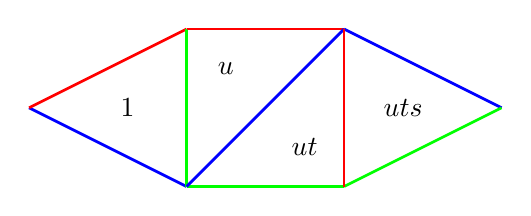
\begin{tikzpicture}[baseline=-0.25cm]
\draw [line width=1pt, blue] (0,0) -- (2,-1);
\draw [line width=1pt, red] (0,0) -- (2,1);
\draw [line width=1pt, green] (2,1) -- (2,-1);
\draw (1.25,0) node [text=black] {$1$};
\draw [line width=1pt, green] (2,-1) -- (4,-1);
\draw [line width=1pt, red] (2,1) -- (4,1);
\draw [line width=1pt, blue] (2,-1) -- (4,1);
\draw (2.5,0.5) node [text=black] {$u$};
\draw (3.5,-0.5) node [text=black] {$ut$};
\draw [line width=1pt, blue] (4,1) -- (6,0);
\draw [line width=1pt, green] (4,-1) -- (6,0);
\draw [line width=1pt, red] (4,1) -- (4,-1);
\draw (4.75,0) node [text=black] {$uts$};
\end{tikzpicture}.
\end{center}
\noindent\\ Suppose we start with $R_w$, for some $w \in {}^KW$. We start by placing a $1$ in the cell corresponding to $w$ and a $0$ in all other cells. Suppose we now wish to act by $B_x$, for some $x \in \{s, t, u\}$. We can imagine this as the following mitotic process. Let $c_{w'}$ be the current value of the cell corresponding to $w' \in {}^KW$. We have that $f_{w'}$, the final value of the cell after acting by $B_x$, is given by ``mitosis'':
\begin{align*}
\begin{split}
f_{w'} \coloneqq c_{w'} + \sum_{w'' \in {}^KW} \delta_{w'}(w''x)c_{w''},
\end{split}
\end{align*}
\noindent where $\delta_{w'}(w''x)$ is equal to $1$ if $w''x \in W_Kw'$ and $0$ otherwise. In other words, each cell duplicates its value across its neighbouring $x$-wall. If crossing this wall should take us outside the diagram, we duplicate in the cell we started in.
\newpage

\noindent For example, $R \otimes_R B_u \otimes_R B_t$ corresponds to\\[-0.5\linespacing]
\begin{center}
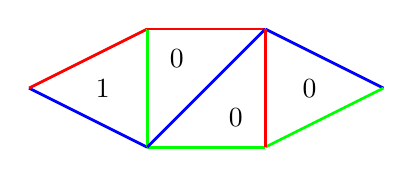
\begin{tikzpicture}[baseline=-0.25cm, x=0.75cm,y=0.75cm]
\draw [line width=1pt, blue] (0,0) -- (2,-1);
\draw [line width=1pt, red] (0,0) -- (2,1);
\draw [line width=1pt, green] (2,1) -- (2,-1);
\draw (1.25,0) node [text=black] {$1$};
\draw [line width=1pt, green] (2,-1) -- (4,-1);
\draw [line width=1pt, red] (2,1) -- (4,1);
\draw [line width=1pt, blue] (2,-1) -- (4,1);
\draw (2.5,0.5) node [text=black] {$0$};
\draw (3.5,-0.5) node [text=black] {$0$};
\draw [line width=1pt, blue] (4,1) -- (6,0);
\draw [line width=1pt, green] (4,-1) -- (6,0);
\draw [line width=1pt, red] (4,1) -- (4,-1);
\draw (4.75,0) node [text=black] {$0$};
\end{tikzpicture}\quad$\overset{-\otimes_R B_u}{\rightsquigarrow}$\quad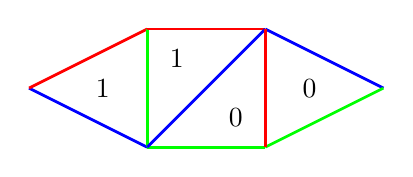
\begin{tikzpicture}[baseline=-0.25cm, x=0.75cm,y=0.75cm]
\draw [line width=1pt, blue] (0,0) -- (2,-1);
\draw [line width=1pt, red] (0,0) -- (2,1);
\draw [line width=1pt, green] (2,1) -- (2,-1);
\draw (1.25,0) node [text=black] {$1$};
\draw [line width=1pt, green] (2,-1) -- (4,-1);
\draw [line width=1pt, red] (2,1) -- (4,1);
\draw [line width=1pt, blue] (2,-1) -- (4,1);
\draw (2.5,0.5) node [text=black] {$1$};
\draw (3.5,-0.5) node [text=black] {$0$};
\draw [line width=1pt, blue] (4,1) -- (6,0);
\draw [line width=1pt, green] (4,-1) -- (6,0);
\draw [line width=1pt, red] (4,1) -- (4,-1);
\draw (4.75,0) node [text=black] {$0$};
\end{tikzpicture}\quad$\overset{-\otimes_R B_t}{\rightsquigarrow}$\quad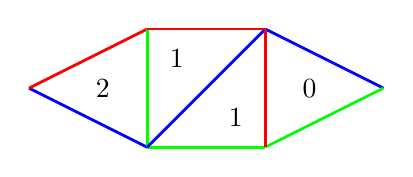
\begin{tikzpicture}[baseline=-0.25cm, x=0.75cm,y=0.75cm]
\draw [line width=1pt, blue] (0,0) -- (2,-1);
\draw [line width=1pt, red] (0,0) -- (2,1);
\draw [line width=1pt, green] (2,1) -- (2,-1);
\draw (1.25,0) node [text=black] {$2$};
\draw [line width=1pt, green] (2,-1) -- (4,-1);
\draw [line width=1pt, red] (2,1) -- (4,1);
\draw [line width=1pt, blue] (2,-1) -- (4,1);
\draw (2.5,0.5) node [text=black] {$1$};
\draw (3.5,-0.5) node [text=black] {$1$};
\draw [line width=1pt, blue] (4,1) -- (6,0);
\draw [line width=1pt, green] (4,-1) -- (6,0);
\draw [line width=1pt, red] (4,1) -- (4,-1);
\draw (4.75,0) node [text=black] {$0$};
\end{tikzpicture}.
\end{center}
\noindent\\ This tells us that\\[-0.5\linespacing]
\begin{center}
$R \otimes_R B_u \otimes_R B_t =$\ 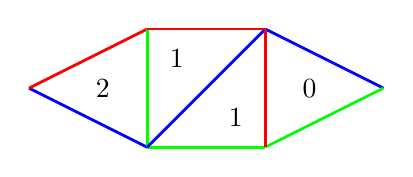
\begin{tikzpicture}[baseline=-0.25cm, x=0.75cm,y=0.75cm]
\draw [line width=1pt, blue] (0,0) -- (2,-1);
\draw [line width=1pt, red] (0,0) -- (2,1);
\draw [line width=1pt, green] (2,1) -- (2,-1);
\draw (1.25,0) node [text=black] {$2$};
\draw [line width=1pt, green] (2,-1) -- (4,-1);
\draw [line width=1pt, red] (2,1) -- (4,1);
\draw [line width=1pt, blue] (2,-1) -- (4,1);
\draw (2.5,0.5) node [text=black] {$1$};
\draw (3.5,-0.5) node [text=black] {$1$};
\draw [line width=1pt, blue] (4,1) -- (6,0);
\draw [line width=1pt, green] (4,-1) -- (6,0);
\draw [line width=1pt, red] (4,1) -- (4,-1);
\draw (4.75,0) node [text=black] {$0$};
\end{tikzpicture}\ \ \!$=$\ 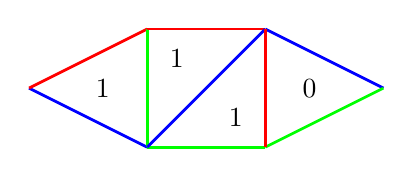
\begin{tikzpicture}[baseline=-0.25cm, x=0.75cm,y=0.75cm]
\draw [line width=1pt, blue] (0,0) -- (2,-1);
\draw [line width=1pt, red] (0,0) -- (2,1);
\draw [line width=1pt, green] (2,1) -- (2,-1);
\draw (1.25,0) node [text=black] {$1$};
\draw [line width=1pt, green] (2,-1) -- (4,-1);
\draw [line width=1pt, red] (2,1) -- (4,1);
\draw [line width=1pt, blue] (2,-1) -- (4,1);
\draw (2.5,0.5) node [text=black] {$1$};
\draw (3.5,-0.5) node [text=black] {$1$};
\draw [line width=1pt, blue] (4,1) -- (6,0);
\draw [line width=1pt, green] (4,-1) -- (6,0);
\draw [line width=1pt, red] (4,1) -- (4,-1);
\draw (4.75,0) node [text=black] {$0$};
\end{tikzpicture} $\oplus\ \!R$.
\end{center}
\noindent\\ Let's try to play a similar game to $R^s \otimes_{R^{s,t}} R$. Without knowing anything about Soergel bimodules in type $A_3$, we may na\"{i}vely expect $R^t \otimes_{R^{t,u}} R$ to be an indecomposable $(R^{s,t}, R)$-bimodule. Well, we can get the generators $\alpha_s + \frac{1}{2}\alpha_t$ and $\alpha_u + \frac{1}{2}\alpha_t$ in $R^t$, as %Indeed, in $A_3$, we have a splitting of $(R, R)$-bimodules
%\begin{align*}
%\begin{split}
%B_t \otimes_R B_u \otimes_R B_t \cong B_{tut} \oplus B_t,
%\end{split}
%\end{align*}
%\noindent for $B_{tut} \coloneqq R \otimes_{R^{t,u}} R(3)$, given by the $(R, R)$-bimodule monomorphisms
%\begin{align*}
%\begin{split}
%B_{tut} &\to B_t \otimes_R B_u \otimes_R B_t : 1 \otimes_{R^{t,u}} 1 \mapsto 1 \otimes_{R^t} 1 \otimes_{R^u} 1\otimes_{R^t} 1,\\
%B_t &\to B_t \otimes_R B_u \otimes_R B_t : 1 \otimes_{R^{t\hphantom{,t}}} 1 \mapsto \frac{1}{2}(1 \otimes_{R^t} (\alpha_t \otimes_{R^u} 1 + 1 \otimes_{R^u} \alpha_t) \otimes_{R^t} 1).
%\end{split}
%\end{align*}
%\noindent This is analogous to the splitting $B_s \otimes_R B_t \otimes_R B_s \cong B_{sts} \oplus B_s$ in type $A_2$. It's easy to show that $R^t \otimes_{R^{t,u}} R$ is indecomposable as an $(R^t, R)$-bimodule, as the same proof from before holds. Our guess is that $R^t \otimes_{R^{t,u}} R$ is moreover indecomposable as an $(R^{s,t}, R)$-bimodule. We just need to show that we can get the generators $\alpha_t^2$, $\alpha_s + \frac{1}{2}\alpha_t$ and $\alpha_u + \frac{1}{2}\alpha_t$ in our copy of $R^t$. First, note that
\begin{align*}
\begin{split}
\frac{1}{4}\left(-\frac{1}{2}\alpha_s - \alpha_t - \frac{3}{2}\alpha_u\right) \otimes_{R^{t,u}} 1 + 1 \otimes_{R^{t,u}} \frac{3}{4}\left(\frac{3}{2}\alpha_s + \alpha_t + \frac{1}{2}\alpha_u\right) = \left(\alpha_s + \frac{1}{2}\alpha_t\right) \otimes_{R^{t,u}} 1,\\
\frac{3}{4}\left(\frac{1}{2}\alpha_s + \alpha_t + \frac{3}{2}\alpha_u\right) \otimes_{R^{t,u}} 1 + 1 \otimes_{R^{t,u}} \frac{1}{4}\left(-\frac{3}{2}\alpha_s - \alpha_t - \frac{1}{2}\alpha_u\right) = \left(\alpha_u + \frac{1}{2}\alpha_t\right) \otimes_{R^{t,u}} 1.\\
\end{split}
\end{align*}
\noindent However, we run into problems with $\alpha_t^2$. First, observe that all order $2$ elements are of the form
\begin{align*}
\begin{split}
\lambda\alpha_s^2 + \mu\alpha_t^2 + 3(\mu - \lambda)\alpha_u^2 + \mu\alpha_s\alpha_t + 2(\mu - \lambda)\alpha_s\alpha_u + 4(\mu - \lambda)\alpha_t\alpha_u &\in R^{s,t},\\
3(\mu' - \lambda')\alpha_s^2 + \mu'\alpha_t^2 + \lambda'\alpha_u^2 + 4(\mu' - \lambda')\alpha_s\alpha_t + 2(\mu' - \lambda')\alpha_s\alpha_u + \mu'\alpha_t\alpha_u &\in R^{t,u}\\
\end{split}
\end{align*}
\noindent for all $\lambda, \mu, \lambda', \mu' \in \mathbb{R}$. Thus, in order to get $\alpha_t^2$, we must solve the system of equations
\begin{align*}
\begin{split}
\lambda + 3(\mu' - \lambda') &= 0,\\
\mu + \mu' &= 1,\\
3(\mu - \lambda) + \lambda' &= 0,\\
\mu + 4(\mu' - \lambda') &= 0,\\
2(\mu - \lambda) + 2(\mu' - \lambda') &= 0,\\
4(\mu - \lambda) + \mu' &= 0.
\end{split}
\end{align*}
\noindent But this system has no solutions! Hence we will need to find a different approach. I still believe that it might be the indecomposable we're looking for though, I don't think any other candidates make sense. By symmetry then we might expect the other remaining indecomposable to be $R^s \otimes_{R^{s,t}} R$. %In fact, through similar reasoning, we find that $R^t \otimes_{R^{s,t}} R$, $R^s \otimes_{R^{s,t}} R$ and $R^s \otimes_{R^{t,u}} R$ are also not indecomposable $(R^{s,t}, R)$-bimodules (and of course we cannot have any subset of $R^u$ on the left, as this is zero as a left $R^{s,t}$-module).
\textcolor{red}{It would be good to check if tensoring these with $B_s$ and $B_u$ respectively gives us $R^{s,t} \otimes_{R^{s,t,u}} R$. It may be the case that these indecomposables don't have a nice, explicit form like this though. Some deeper insight from $\mathbb{S}\textcat{Bim}(A_3)$ would help a lot here.}
\newpage

\noindent Using Anna's method, we can fill out the rest of the $W$-graph as\\[7\linespacing]
\begin{center}
\begin{tikzcd}[overlay, labels={outer sep=-1cm}, nodes={circle, minimum size=2.5cm, inner sep=-0.25cm, outer sep=-0.75cm}, cramped, column sep=-0.75cm, row sep=-0.75cm]
& & & R^{s,t} \otimes_{R^{s,t,u}} R\arrow[out=60, in=120, loop, looseness=5, "{s,t,u}"'] & & &\\
% & & R \otimes_R B_{ut}\arrow[dl, shift right, "s"']\arrow[ur, "s"']\arrow[out=80, in=140, loop, looseness=5, "{t,u}"'] & & R_u \otimes_R B_{ts}\arrow[ul, "u"']\arrow[dr, shift right, "u"']\arrow[out=40, in=100, loop, looseness=5, "{s,t}"'] & &\\
% & & \textcolor{red}{R^{s,t} \otimes_{R^{t,u}} R}\arrow[dl, shift right, "s"']\arrow[ur, "s"']\arrow[out=80, in=140, loop, looseness=5, "{t,u}"'] & & \textcolor{red}{?}\arrow[ul, "u"']\arrow[dr, shift right, "u"']\arrow[out=40, in=100, loop, looseness=5, "{s,t}"'] & &\\
& & \textcolor{red}{R^t \otimes_{R^{t,u}} R}\arrow[dl, shift right, "s"']\arrow[ur, "s"']\arrow[out=80, in=140, loop, looseness=5, "{t,u}"'] & & \textcolor{red}{R^s \otimes_{R^{s,t}} R}\arrow[ul, "u"']\arrow[dr, shift right, "u"']\arrow[out=40, in=100, loop, looseness=5, "{s,t}"'] & &\\
& R \otimes_R B_u\arrow[ur, shift right, "t"']\arrow[dl, shift right, "t"']\arrow[out=80, in=140, loop, looseness=5, "{s,u}"'] & & R_u \otimes_R B_t\arrow[dl, shift right, "s"']\arrow[ur, "s"']\arrow[dr, shift right, "u"']\arrow[ul, "u"']\arrow[out=60, in=120, loop, looseness=5, "{t}"'] & & R_{ut} \otimes_R B_s\arrow[dr, shift right, "t"']\arrow[ul, shift right, "t"']\arrow[out=40, in=100, loop, looseness=5, "{s,u}"'] &\\
R\arrow[ur, shift right, "u"']\arrow[out=220, in=280, loop, looseness=5, "{s,t}"'] & & R_u\arrow[ul, "u"']\arrow[ur, shift right, "t"']\arrow[out=240, in=300, loop, looseness=5, "{s}"'] & & R_{ut}\arrow[ur, "s"']\arrow[ul, shift right, "t"']\arrow[out=240, in=300, loop, looseness=5, "{u}"'] & & R_{uts}\arrow[ul, shift right, "s"']\arrow[out=260, in=320, loop, looseness=5, "{t,u}"']
% & & & Q_9 & & &\\
% & & Q_7 & & Q_8 & &\\
% & Q_4 & & Q_5 & & Q_6 &\\
% Q_2 & & Q_0 & & Q_1 & & Q_3
\end{tikzcd}
\end{center}
\begin{center}
\noindent\\[-2\linespacing]\qquad\qquad\qquad\qquad\qquad\qquad\qquad\qquad\qquad\qquad\qquad\qquad\qquad\qquad\qquad\qquad.
\end{center}
\noindent\\[7.25\linespacing] I'm wondering if the module categories generated by the leftmost and rightmost legs are equivalent. I assume either they always are or never are, but without knowing the morphisms in these weird quotient categories it's impossible to say. This may be easier to answer if you know the Lusztig--Vogan module well enough. I would expect this pattern to repeat. This is also notably the first example where the Lusztig--Vogan category does not contain every simple transitive $\mathbb{S}\textcat{Bim}$-module category as a composition quotient, as type $A_3$ Coxeter systems have $5$ two-sided cells.
\end{example}
\newpage

\noindent\begin{example}\textup{($G_\mathbb{R} = G_{2(2)}$).} The Weyl group for $G_2$ is well known to be
\begin{align*}
\begin{split}
D_6 \coloneqq \langle s, t : s^2 = t^2 = (st)^6 = 1\rangle,
\end{split}
\end{align*}
\noindent the dihedral group of order $12$. In \cite[Theorem 1.10.1]{Yok25}, it is shown that the fixed-point subgroup of split $G_2$ under its Cartan involution is $(\textup{Sp}(1) \times \textup{Sp}(1))/\mathbb{Z}_2 \cong \textup{SO}(4)$. The fixed-point subgroup of complex $G_2$ under this Cartan involution is then $K = \textup{SL}(2, \mathbb{C}) \times \textup{SL}(2, \mathbb{C})$ -- the complexification of $\textup{SO}(4)$ -- giving us $W_K = \mathbb{Z}/2\mathbb{Z} \times \mathbb{Z}/2\mathbb{Z}$. Both $K$ and complex $G_2$ have a maximal torus of rank $2$, landing us in the equal rank case. At this stage, we are not sure how $W_K$ lives inside $W$. Indeed, there are three distinct copies of the Klein four-group $\mathbb{Z}/2\mathbb{Z} \times \mathbb{Z}/2\mathbb{Z}$ living inside $D_6$; these are
\begin{align*}
\begin{split}
\langle s,\hphantom{(st)^0} (st)^3\rangle &= \{1, ststst, tstst, s\},\\
\langle s(st)^2, (st)^3\rangle &= \{1, ststst, sts, tst\},\\
\langle s(st)^4, (st)^3\rangle &= \{1, ststst, ststs, t\}.
\end{split}
\end{align*}
\noindent Because $\abs{W_K\backslash W} = 3$, we know that $W_K\backslash W \cong \mathbb{Z}/3\mathbb{Z}$. Computing the right cosets, we have\\[-0.5\linespacing]
\begin{center}
\renewcommand{\arraystretch}{1.5}
\begin{tabular}{|l|l|}
\hline
\rowcolor[HTML]{EFEFEF} 
$H$ & \multicolumn{1}{c|}{\cellcolor[HTML]{EFEFEF}$H\backslash D_6$} \\\hline
$\langle s,\hphantom{(st)^0} (st)^3\rangle$ & $\{H, Ht, Hts\}$\\\hline
$\langle s(st)^2, (st)^3\rangle$ & $\{H, Hs, Ht\}$\\\hline
$\langle s(st)^4, (st)^3\rangle$ & $\{H, Hs, Hst\}$\\\hline
\end{tabular}\ .\\[0.5\linespacing]
\renewcommand{\arraystretch}{1}
\end{center}
\noindent By symmetry, we therefore only have two choices of right coset representatives. My guess is that ${}^KW = \{1, s, t\}$, although we would have to use the root systems to know for certain. Anna might have something about this in \cite[Lemma 6.1.3]{LR22}.\\

\noindent To-do: right now, a lot of these problems are kind of tough. I think the best way to proceed would be to think about the analogue of standard filtrations and formalize Anna's method / see what else we can learn from them. It would also be good to prove that you always have an indecomposable of the form $R^{W_K} \otimes_{R^W} R$.\\

\noindent For $G_2$, I'd like to compute its ``categorical $W$-graph'' and check if it looks different to the decategorified $W$-graph. Then I'd like to check if $G_2$ has non-cell simple transitive module subcategories.\\

\noindent Long-term: move beyond Weyl groups (akin to Soergel's conjecture vs. the Kazhdan--Lusztig conjecture).
\end{example}
\newpage

\renewcommand\thesection{R}
\ruledsectionstar{References}{References}
\begingroup
\setlength{\emergencystretch}{.5em}
\printbibliography[heading=none]
\endgroup
\newpage

%\vspace*{\fill}
%\hfill Page intentionally left blank. \hfill
%\vspace*{\fill}
%\newpage

%\phantomsection\addcontentsline{toc}{section}{Talks}
%\noindent\\\textbf{Motivation}
%\begin{enumerate}[label=$\bullet$, leftmargin=1\parindent]
%\item What is finitary birepresentation theory? My take: a ``categorification'' of the representation theory of finite-dimensional algebras, arising from the study of knot invariants, tensor categories and operator algebras. In other words, Jones mathematics (lol).
%\item Stealing some slogans from one of Dani's talks: representation theory is group theory in vector spaces, while birepresentation theory is group theory in linear categories.
%\item Why is it important? Basically for (somehow) studying the fields I just mentioned. Hopefully by the end of this little series we can figure out the answer to this together.\\
%\end{enumerate}

%\noindent\textbf{Plan}
%\begin{enumerate}[label=$\bullet$, leftmargin=1\parindent]
%\item Today I'd like to introduce one of the main theorems of birepresentation theory: the ``weak Jordan-- H\"{o}lder theorem''. This theorem is a nice (abstract) motivation for the classification of simple birepresentations.
%\item In principle I'm not sure how helpful this talk will be. It will mostly be walking you through what I've been thinking about over the past couple of weeks. The main theorem is, I think, quite nice, but getting there will likely be dry. Next time I'd like to focus more on examples (especially Soergel bimodules and their classification) if I'm capable enough.
%\item Addressing a question: why am I talking about birepresentations? The people were promised $2$-representations! In classifying $2$-representations of Soergel bimodules, it was quickly found that the language of $2$-representations was too restrictive. Later on in this series I will probably transition to $2$-representations, but at least in this talk I'd like to state things as generally as possible to avoid issues later on.
%\item As a reminder to myself, I'd like to maintain a little definition bank so you guys can keep track of definitions.\\
%\end{enumerate}

%\noindent\textbf{Multifinitary Categories}
%\begin{enumerate}[label=$\bullet$, leftmargin=1\parindent]
%\item What are multifinitary $1$-categories? Add this to the definition bank.
%\item In linear algebra, all idempotents split. Idempotent complete categories live somewhere between additive categories and Abelian categories. In particular, {\em all pseudo-Abelian categories are\linebreak idempotent complete!} These remarks are what ``unlocked'' idempotent completeness for me.
%\item Examples of finitary categories (that I can't write down because I haven't prepared any concrete examples): (semi)groups and their representations, quantum groups and their categorifications, tensor categories, fusion categories, modular (tensor) categories, $2$-Kac-Moody categories, etc.
%\item $\textsf{Vect}_\mathbbm{k}$ is a helpful example: $\begin{pmatrix}1&0\\0&0\end{pmatrix} = \begin{pmatrix}1\\0\end{pmatrix}\!\begin{pmatrix}1&0\end{pmatrix}$.
%\item Maybe mention example 2.8? Mazorchuk and Miemietz would have you believe it's a useful example but man is it impenetrable.
%\item Also, $\mathbb{S}\textsf{Bim}(W, S)$ lololol
%\item Define the category of multifinitary categories.
%\item Finitary bicategories. Add this to the definition bank. We can generate these from finitary monoidal categories: in particular, there is a bijection between monoidal categories and one-object bicategories, with delooping taking us upstairs and Hom-categories taking us downstairs. Mention strict case.
%\end{enumerate}
%\newpage

%\noindent\textbf{Finitary Birepresentations}
%\begin{enumerate}[label=$\bullet$, leftmargin=1\parindent]
%\item What are finitary birepresentations? There is a bijection between module categories and\linebreak birepresentations of one-object bicategories. Example: Yoneda birepresentations.
%\item Equivalence of birepresentations. I don't understand these very well yet.\\
%\end{enumerate}

%\noindent\textbf{Simple Birepresentations}
%\begin{enumerate}[label=$\bullet$, leftmargin=1\parindent]
%\item Walk through next block: essentially, I want to define what it means for a birepresentation to be transitive. If you're like me and you keep forgetting what this adjective means, an action of $G$ on a set $X$ is said to be transitive if, for any $x, y \in X$, there is some $g \in G$ for which $g \cdot x = y$.
%\item Define transitive birepresentations. Add this to the definition bank. What are we trying to capture with transitivity?
%\item There is a ``better'' notion of simplicity.
%\item What are ideals of finitary $1$-categories? Mention that I've talked to Dani about this and they gave a somewhat confusing answer, but I think I've figured it out. I'm mentioning this in case I'm actually stupid.
%\item Give an example -- $\textsf{Vect}_\mathbbm{k}$ yippeeee!!
%\item What are $\mathscr{C}$-stable ideals of birepresentations?
%\item What are simple birepresentations? Add this to the definition bank. Why are they ``better''? They somehow more completely characterize what it means for a representation to be simple. Unfortunately, I don't really have an example of a non-simple transitive birepresentation for you right now asides from Lusztig--Vogan module categories, but I'll hopefully have one next week. Many of the na\"{i}ve examples of transitive birepresentations end up being simple.
%\item Result I'll need: transitive birepresentations admit a unique maximal ideal, and quotienting by this ideal gives you a simple birepresentation. We call this the simple quotient of $\textup{M}$. Run through a sketch of the proof.\\
%\end{enumerate}

%\noindent\textbf{Weak Jordan--H\"{o}lder}
%\begin{enumerate}[label=$\bullet$, leftmargin=1\parindent]
%\item Define $\textup{Ind}(\textup{M})$, note that it is finite. Define preorder, outline the proof. Recall: preorder means $X \geq X$ and $X \geq Y, Y \geq Z \implies X \geq Z$. Quotienting by $X \sim Y \iff X \geq Y, Y \geq X$ gives us an honest partial order (pretty much by definition).
%\item Proposition: $\textup{M}$ is transitive if and only if $\abs{\textup{Ind}(\textup{M})/\!\sim} = 1$..
%\item Define poset ideal and coideal.
%\item Maybe now would be a good time to remind everyone of the classical Jordan--H\"{o}lder theorem. Given a representation $\textup{M}$, we would like a sensible notion of composition series.
%\item How do coideals induce sub-birepresentations?
%\item How do pairs of coideals induce transitive birepresentations?
%\item How can we make these birepresentations simple?
%\item State the theorem and run through a sketch of the proof.
%\end{enumerate}
%\newpage

\end{document}